\label{ch:neutronics}

This chapter presents several studies that use Moltres as a stand-alone neutronics solver.
The objective of the chapter is to validate Moltres' calculation scheme by comparing Moltres results to Serpent and the OECD/NEA MHTGR-350 Benchmark.
This chapter comprises the following sections: Section \ref{sec:neut-prelim} describes preliminary studies that help set up Serpent and Moltres simulations, Section \ref{sec:neut-serpent} presents several studies comparing Moltres and Serpent results, Section \ref{sec:ph1e1} discusses Moltres results of Phase I Exercise 1 of the benchmark, and Section \ref{sec:neutr-conc} concludes the chapter with a summary of the chapter and its key points.

\section{Preliminary studies}
\label{sec:neut-prelim}

This section's purpose is to determine the proper setup of Serpent and Moltres simulations.
Section \ref{sec:homo-hetero} focuses on the definition of the materials in Serpent input file for obtaining the group constants for Moltres.
Section \ref{sec:setup} analyzes different ways to set up Moltres input files.

\subsection{Homogeneous vs. heterogeneous isotope distribution}
\label{sec:homo-hetero}

This section determines the proper way to treat the fuel compact heterogeneities in Serpent.
This study modeled in Serpent two different material distributions in a fuel compact: a homogeneous distribution of the isotopes and a heterogeneous distribution that explicitly modeled the TRISO particles.
The study used a hexagonal unit cell model that included the fuel compact, a helium gap, and the surrounding graphite, exhibited in Figure \ref{fig:compact-model}.
Table \ref{tab:compact} specifies the model input parameters.
The material temperature was 1200K, a case that represents the \gls{HFP} core state \cite{strydom_results_2015}.
The Serpent simulations included 5$\times 10^4$ neutrons per cycle, 500 active cycles, and 50 inactive cycles for the calculations.
The homogeneous distribution simulation took 1.73 minutes and the heterogeneous distribution simulation 2.21 minutes using 256 cores --- the heterogeneous calculation took 28$\%$ longer.

\begin{figure}[htbp!]
  \centering
    \subfloat[Homogeneous isotope distribution in the fuel compact.]{
        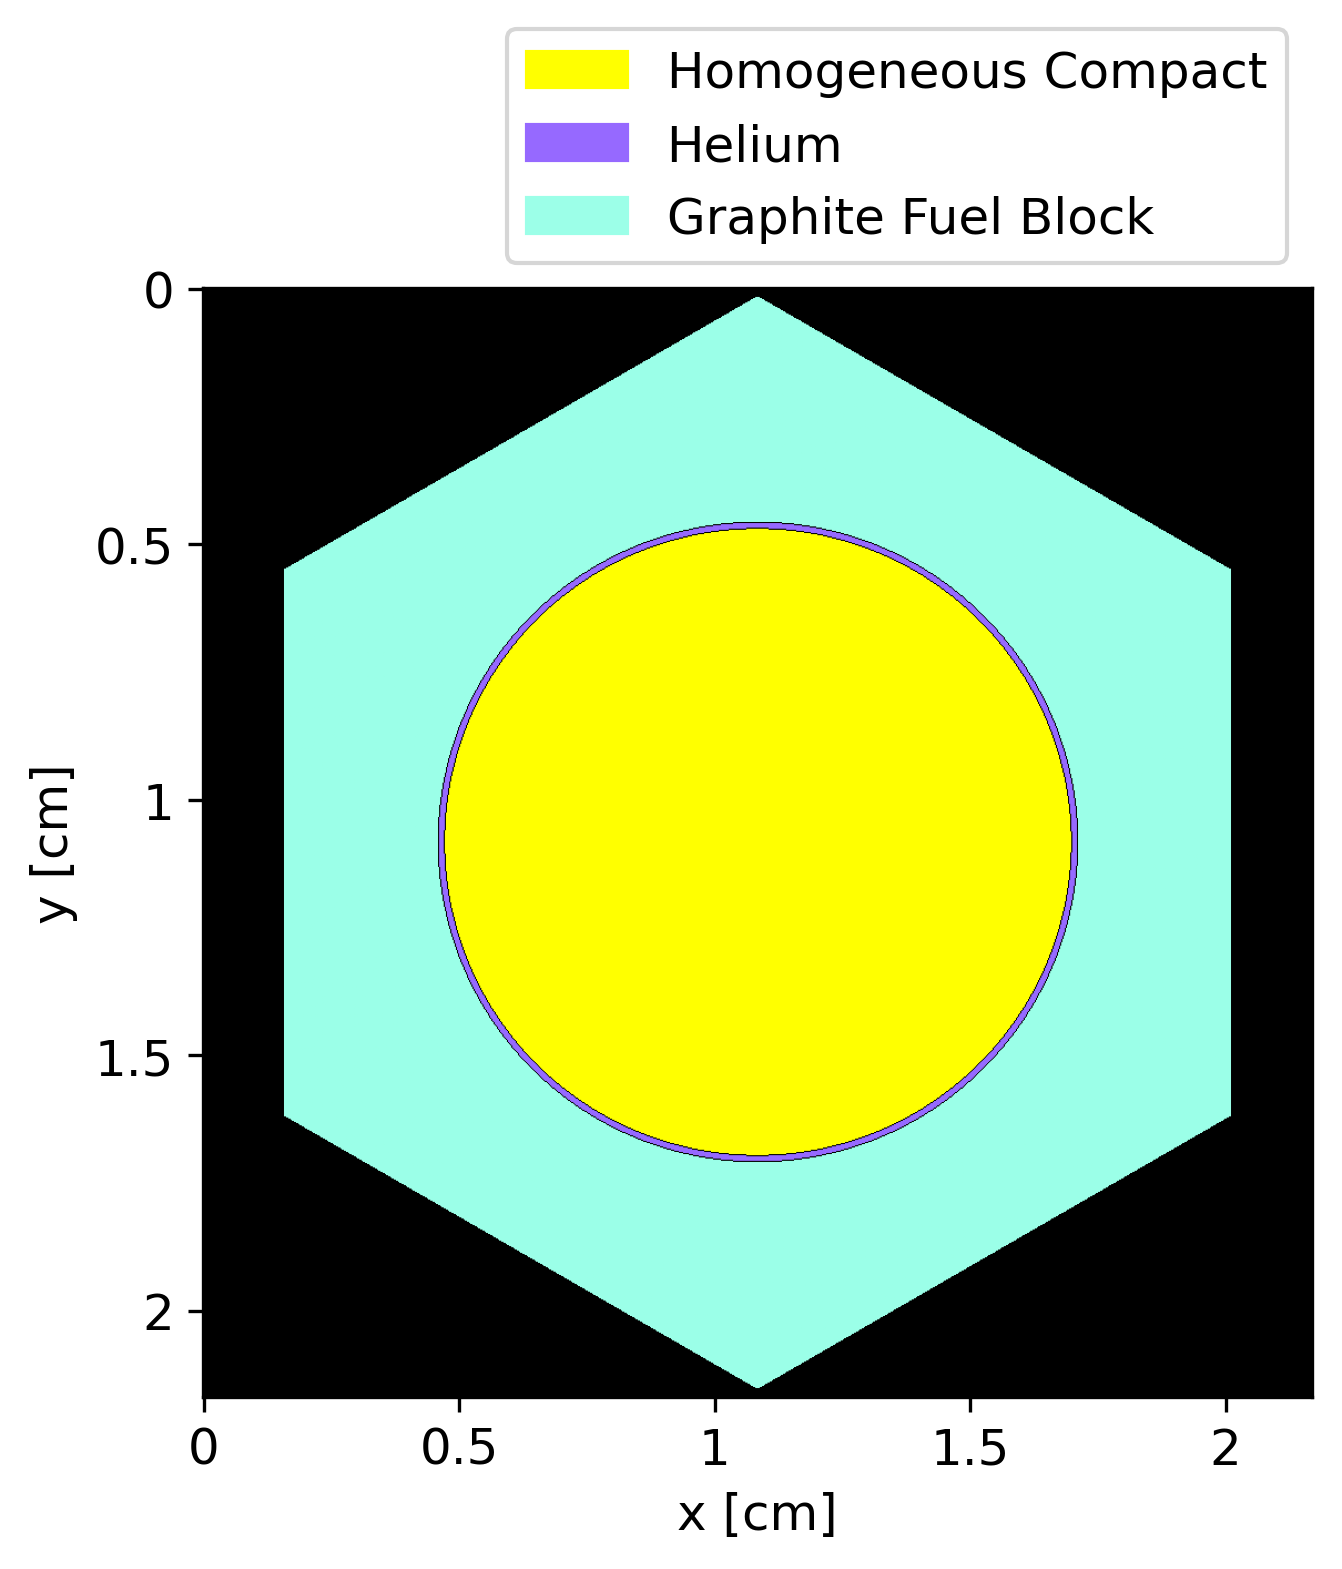
\includegraphics[width=0.45\textwidth]{figures-neutronics/compact-homo}
    }
    \subfloat[Explicit model of the TRISO particles in the fuel compact.]{
        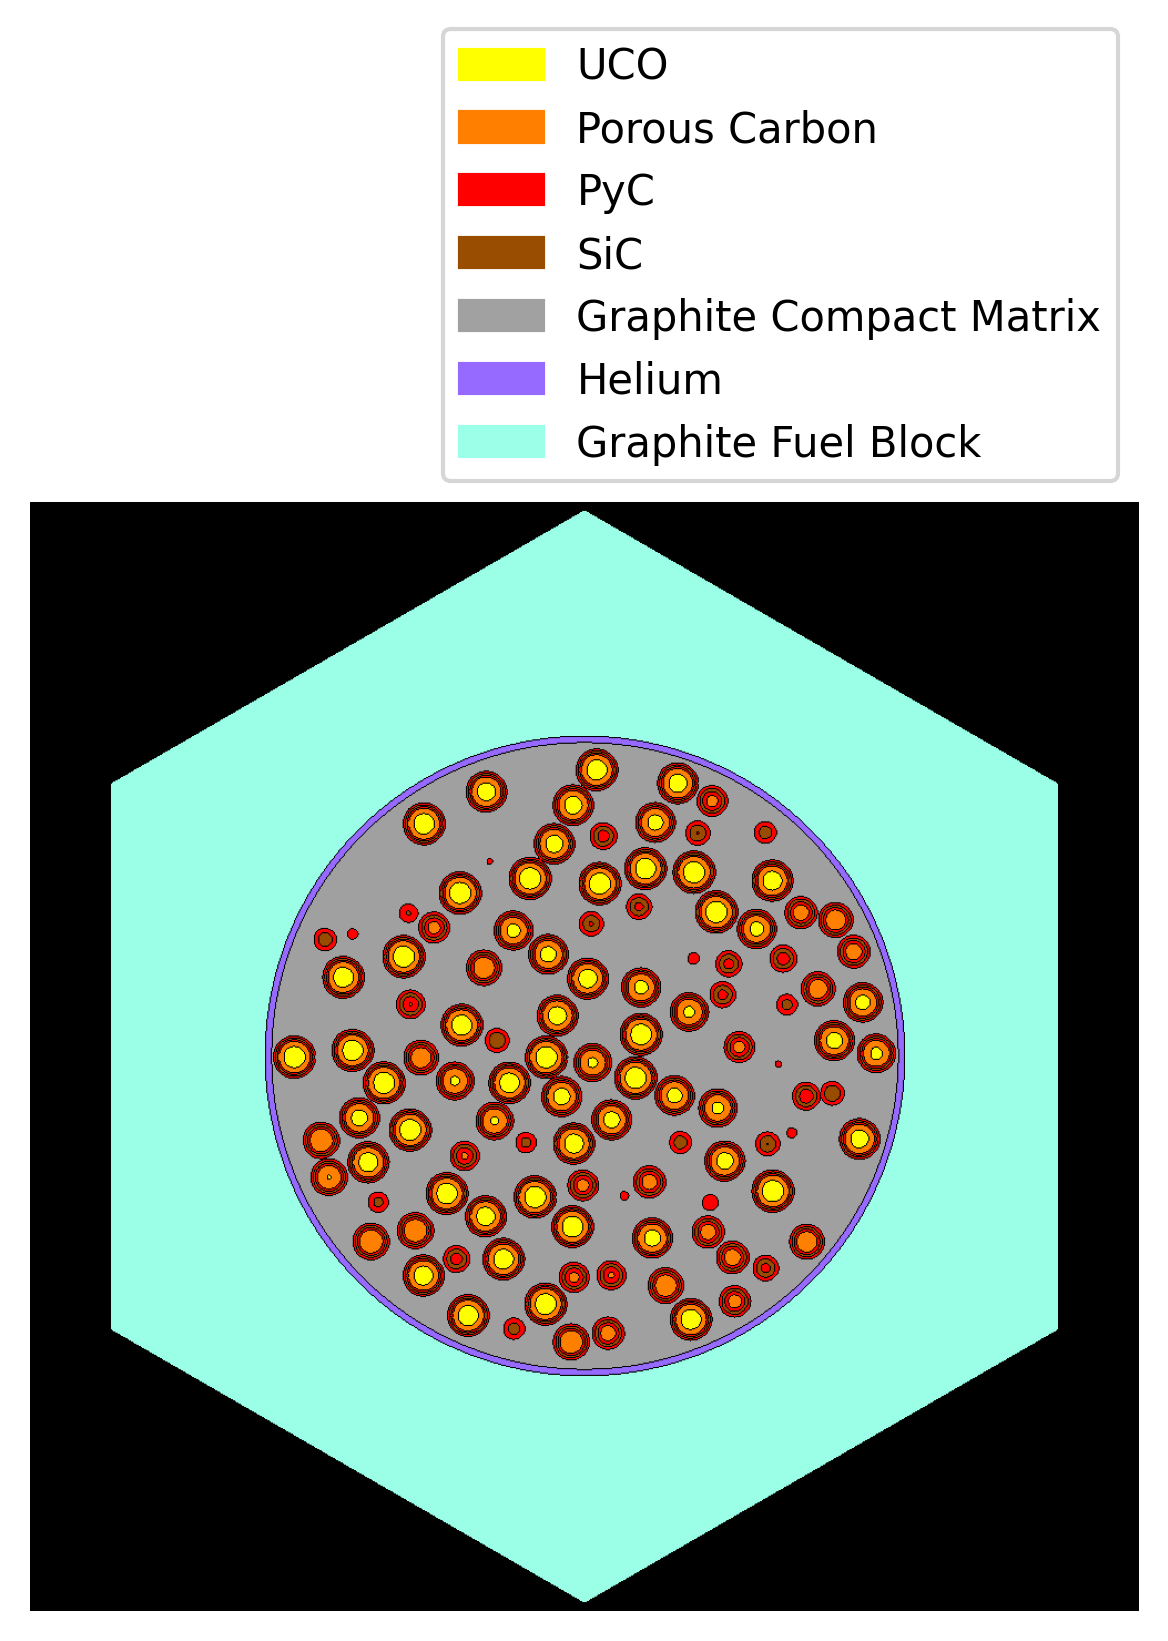
\includegraphics[width=0.45\textwidth]{figures-neutronics/compact}
    }
  \hfill
  \caption{Comparison of different Serpent models of the fuel compact.}
  \label{fig:compact-model}
\end{figure}

The \gls{Keff} was 1.17527 $\pm$ 0.00021 for the homogeneous distribution and 1.25107 $\pm$ 0.00020 for the heterogeneous distribution.
Serpent generated the group constants using the three energy group structure [0, 2.38eV, 111keV, 20MeV].
Figure \ref{fig:param-comparison} displays the group constants' relative error.
The evaluated parameters were $D_g$, $\Sigma^r_g$, $\nu\Sigma^f_g$, and $\chi^t_g$ (see Equation \ref{eq:diffusion-eig}).
Figure \ref{fig:param-comparison} displays the relative errors for $\Sigma^r_g$ and $\nu\Sigma^f_g$, which were the group constants that changed the most.
The relative errors of $\Sigma^r_g$ and $\nu\Sigma^f_g$ were less than 6$\%$, while $D_g$ and $\chi^t_g$ relative errors were less than 1$\%$.

\begin{figure}[htbp!]
	\centering
	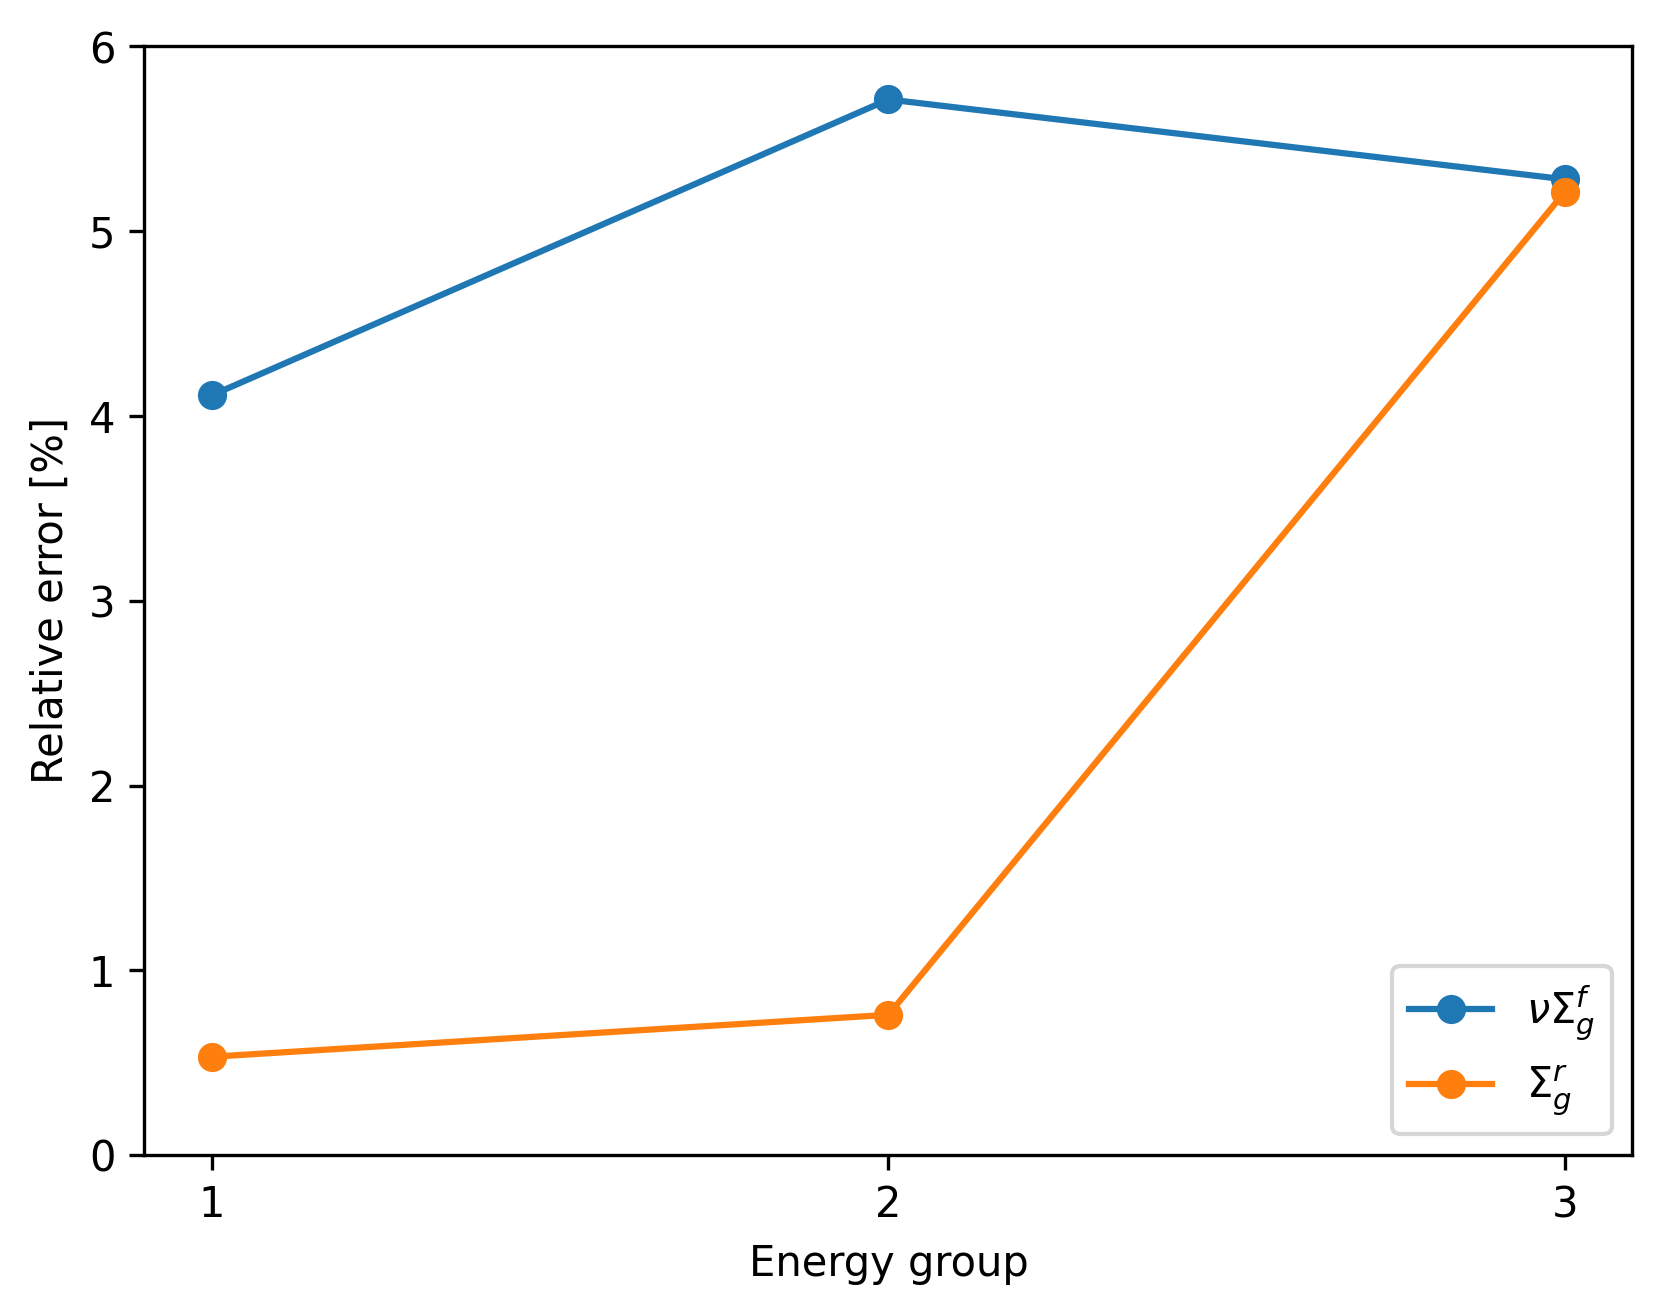
\includegraphics[width=0.43\linewidth]{figures-neutronics/param-comparison}
	\hfill
	\caption{Relative error of the group constants generated with a homogeneous isotope distribution vs. explicit TRISO modeling.}
	\label{fig:param-comparison}
\end{figure}

The results show that the homogenization of the fuel compact isotopes decreases the multiplication factor considerably.
Although the group constant variation is smaller than 6\%, it has a significant impact on the multiplication factor.
Based on these results, Serpent models the TRISO particles explicitly for generating the group constants in the following sections.

\subsection{Problem setup}
\label{sec:setup}

% Diffusion calculations: homo vs hetero in LWRs
Diffusion calculations necessitate a spatial homogenization of the group constants.
Depending on the desired level of detail, the type of homogenization could vary.
For example, in PWR core calculations, the homogenization in space could be per assembly or pin-by-pin \cite{krebs_calculational_1990}.
In a per-assembly homogenization, the diffusion solver represents the assembly as a single material neutronically (we will refer to diffusion calculations using this type as homogeneous calculations).
A pin-by-pin homogenization treats the pin or assembly heterogeneities, yielding a more detailed neutronic representation of the fuel assembly (we will refer to diffusion calculations of this type as heterogeneous calculations).

% Previous works using Moltres
Previous work \cite{lindsay_introduction_2018}\cite{pater_multiphysics_2019} used Moltres for simulating \glspl{MSR}, which allow for heterogeneous calculations.
Keeping in mind Moltres proven capabilities, this work aimed for a heterogeneous calculation of a prismatic \gls{HTGR}.
For this study, Serpent modeled a fuel column of the MHTGR-350 and generated the group constants.
Figure \ref{fig:fuelcolumn} displays the Serpent model geometry.
Serpent generated the group constants for three materials: moderator, coolant, and fuel compact.
The Serpent simulations included 5$\times 10^5$ neutrons per cycle, 400 active cycles, and 100 inactive cycles for the calculations.
% The \gls{Keff} was 1.41933.
Taking advantage of the problem's symmetry, Moltres modeled only $1/12^{th}$ of the fuel column, shown in Figure \ref{fig:fuelcolumn}.
Gmsh \cite{geuzaine_gmsh_2020} produced the geometry and mesh.
The diffusion calculation had 1.84$\times 10^5$ \glspl{DoF} per energy-group.

\begin{figure}[htbp!]
	\centering
    \subfloat[Serpent model geometry.]{
        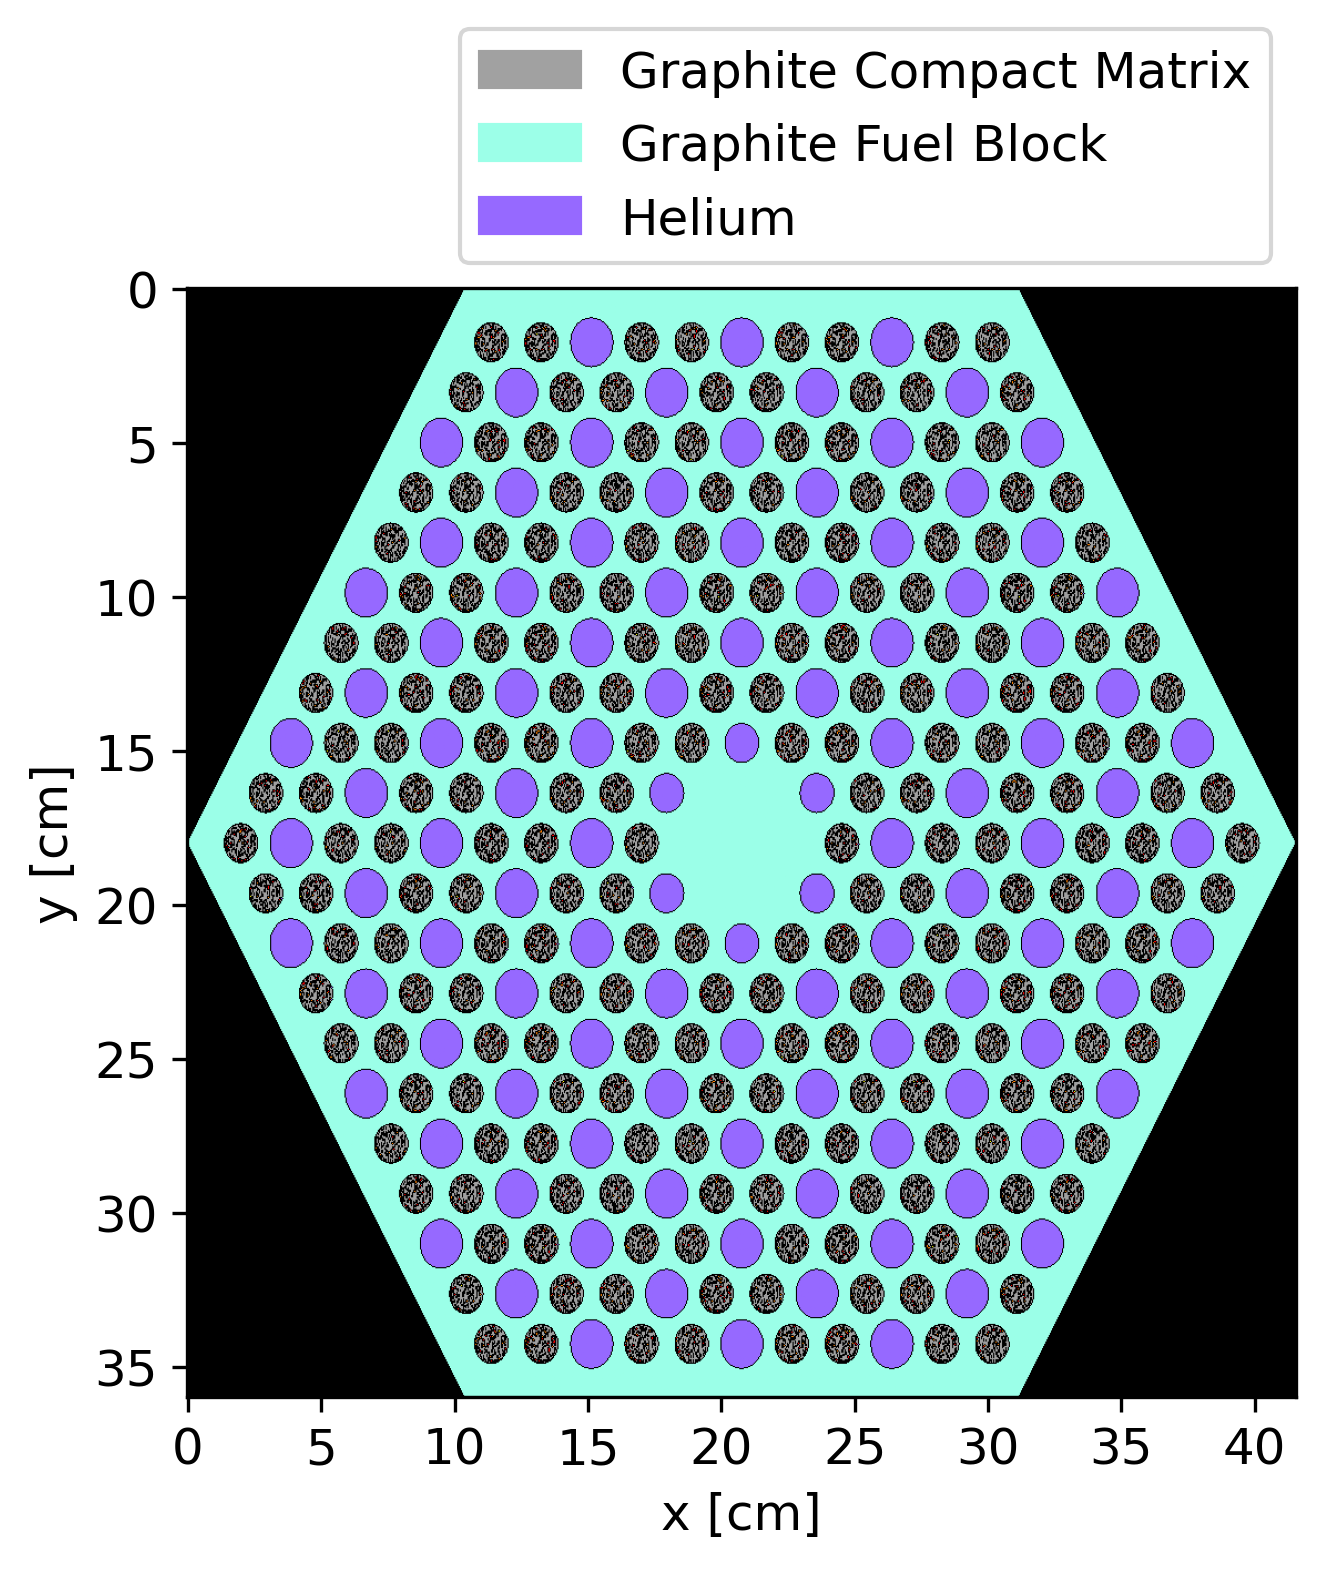
\includegraphics[width=0.42\textwidth]{figures-neutronics/standard}
    }
    \subfloat[Moltres model geometry.]{
        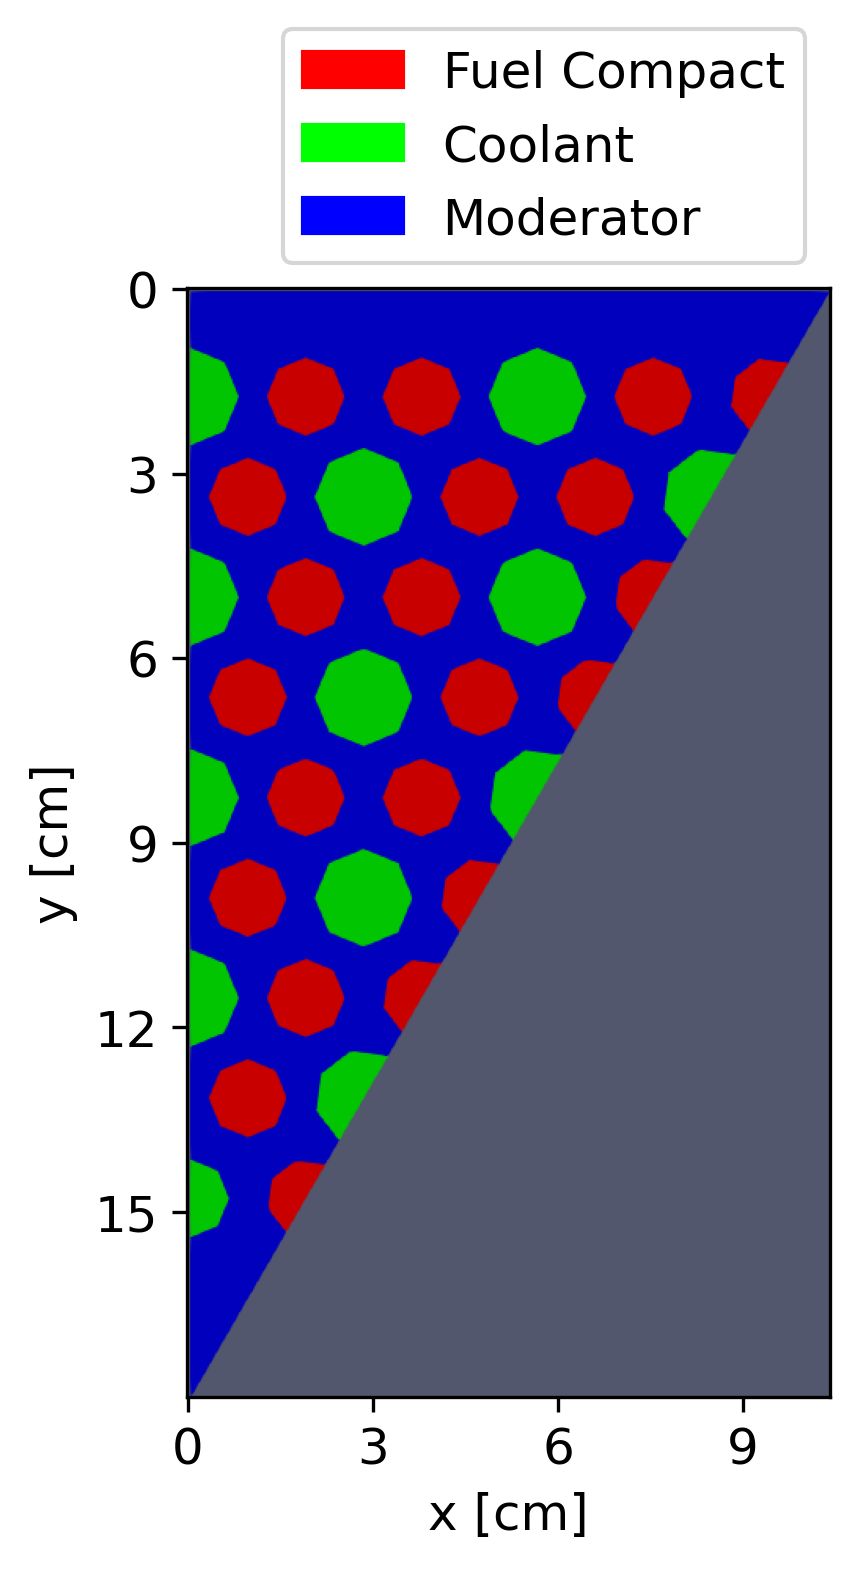
\includegraphics[width=0.27\textwidth]{figures-neutronics/3D-assembly-30deg-reflec-meshB2}
    }
	\hfill
    \caption{Fuel column of the MHTGR-350. $xy$-plane in the active core region.}
	\label{fig:fuelcolumn}
\end{figure}

Moltres input files set an eigenvalue convergence tolerance of 10$^{-8}$, defined by equation \ref{eq:moltres-tol}

\begin{align}
   & \frac{k^{(n)}-k^{(n-1)}}{k^{(n)}} < \varepsilon \label{eq:moltres-tol}
   \intertext{where}
   & k^{(n)} = \mbox{eigenvalue at iteration $n$ } [-] \notag \\
   & \varepsilon = \mbox{convergence tolerance } [-]. \notag
\end{align}

The calculation used two energy groups with the structure [0, 0.625eV, 20MeV].
The eigenvalue calculation did not converge.
Although several factors could contribute to this behavior, this analysis focused on the validity of the diffusion calculations in this system.

% Diffusion validity see bu1/tools-bu.txt
In diffusion theory, the current density $J$ is proportional to the gradient of the flux \cite{leppanen_development_2007}
\begin{align}
   & J = - D \nabla \phi \label{eq:diff} \\
   \intertext{where}
   & J = \mbox{current density } [n \cdot cm^{-2} \cdot s^{-1}] \notag \\
   & D = \mbox{diffusion coefficient } [cm] \notag \\
   & \phi = \mbox{neutron flux } [n \cdot cm^{-2} \cdot s^{-1}]. \notag
\end{align}

This approximation relies on the following assumptions:
\begin{itemize}
	\item the angular flux does not depend strongly on the angular variables,
	\item the fission source is isotropic,
	\item the time derivative of the current density is small compared to the mean collision time,
	\item and the anisotropic energy-transfer due to scattering is negligible in group-to-group scattering.
\end{itemize}

More detailed studies of the transport equation indicate that the following cases violate the assumption of a weak angular dependence \cite{duderstadt_nuclear_1976}:
\begin{itemize}
    \item regions near vacuum boundaries and low-density material regions,
    \item regions near strongly absorbing media,
    \item and regions near localized sources.
\end{itemize}

The diffusion theory applies best to geometries consisting of large homogeneous regions where the flux gradient is small, which is the case for material regions whose geometrical scales are considerably larger than the neutron mean free path.
For this reason, Table \ref{tab:mfp} compares the neutron mean free path in the different fuel assembly materials.
The mean free path in the fuel compact and the moderator are in the order of the centimeters, while in the coolant, the mean free path is comparable to the fuel column dimensions.
These results suggest that a heterogeneous diffusion calculation of the prismatic fuel column challenges some of the diffusion theory assumptions.

\begin{table}[htbp!]
  \centering
  \caption{Neutron mean free path in different materials. Values expressed in [$cm$].}
  \begin{tabular}{lcccc}
  \toprule
              & Fuel compact  & Moderator  & Coolant  & Homogeneous fuel \\
  \midrule
  Fast  		  & 2.71 & 2.70 & 1137.31 & 3.37 \\
  Thermal		  & 2.22 & 2.36 & 1945.49 & 2.89 \\
  \bottomrule
  \end{tabular}
  \label{tab:mfp}
\end{table}

Next, the analysis studied a homogeneous calculation of the fuel assembly in Moltres.
Serpent calculated the fuel assembly's homogeneous group constants by homogenizing the fuel, coolant, and moderator.
This material's mean free path is in the order of the centimeters, shown in Table \ref{tab:mfp}.
Next, Moltres simulation used the homogeneous group constants to carry out an eigenvalue calculation.
Comparing Moltres results with Serpent results, Serpent's \gls{Keff} was 1.41942 $\pm$ 0.00007 while Moltres' was 1.40788.
Equation \ref{eq:delta-rho} calculates the reactivity difference ($\Delta \rho$) between the eigenvalues calculated by Serpent and Moltres
\begin{align}
  & \Delta \rho = \left| \rho_1 - \rho_2 \right| = \left| \frac{k_1-1}{k_1} - \frac{k_2-1}{k_2} \right| = \left| \frac{k_1-k_2}{k_1 k_2} \right| \label{eq:delta-rho} \\
  \intertext{where}
  & k_1 = \mbox{Serpent-derived eigenvalue} [-] \notag \\
  & k_2 = \mbox{Moltres-derived eigenvalue} [-]. \notag
\end{align}

The eigenvalue calculated by Moltres is 577 pcm smaller than the calculated by Serpent.
% This difference is possibly due to the lack of treatment of the anisotropic term in the scattering cross-section.
Additionally, Figure \ref{fig:prelim} displays the axial flux in the fuel column obtained with Serpent and Moltres.
Note that Serpent's flux is the average value of the flux in each bin of the detector, while Moltres flux is the point-wise flux over the $z$-axis
\begin{align}
  & \phi_s(z) = \frac{\int_{\Delta V} \phi(x,y,z) dV}{\Delta V} \label{eq:serpent-flux} \\
  & \phi_m(z) = \phi(x,y,z)   \label{eq:moltres-flux}
  \intertext{where}
  & \phi_s(z) = \mbox{Serpent axial flux } [n \cdot cm^{-2} \cdot s^{-1}] \notag \\
  & \Delta V = \mbox{volume of the detector bins } [cm^3] \notag \\
  & \phi_m(z) = \mbox{Moltres axial flux } [n \cdot cm^{-2} \cdot s^{-1}]. \notag
\end{align}

The fluxes are similar in shape and magnitude.
% Conclusion
Emphasizing that this was a feasibility, the analysis remains qualitative and the following sections present a more in-depth analysis of more detailed results.
Based on these results and discussion, the following sections study homogeneous calculations using Moltres.

\begin{figure}[htbp!]
	\centering
    \subfloat[Serpent axial flux.]{
        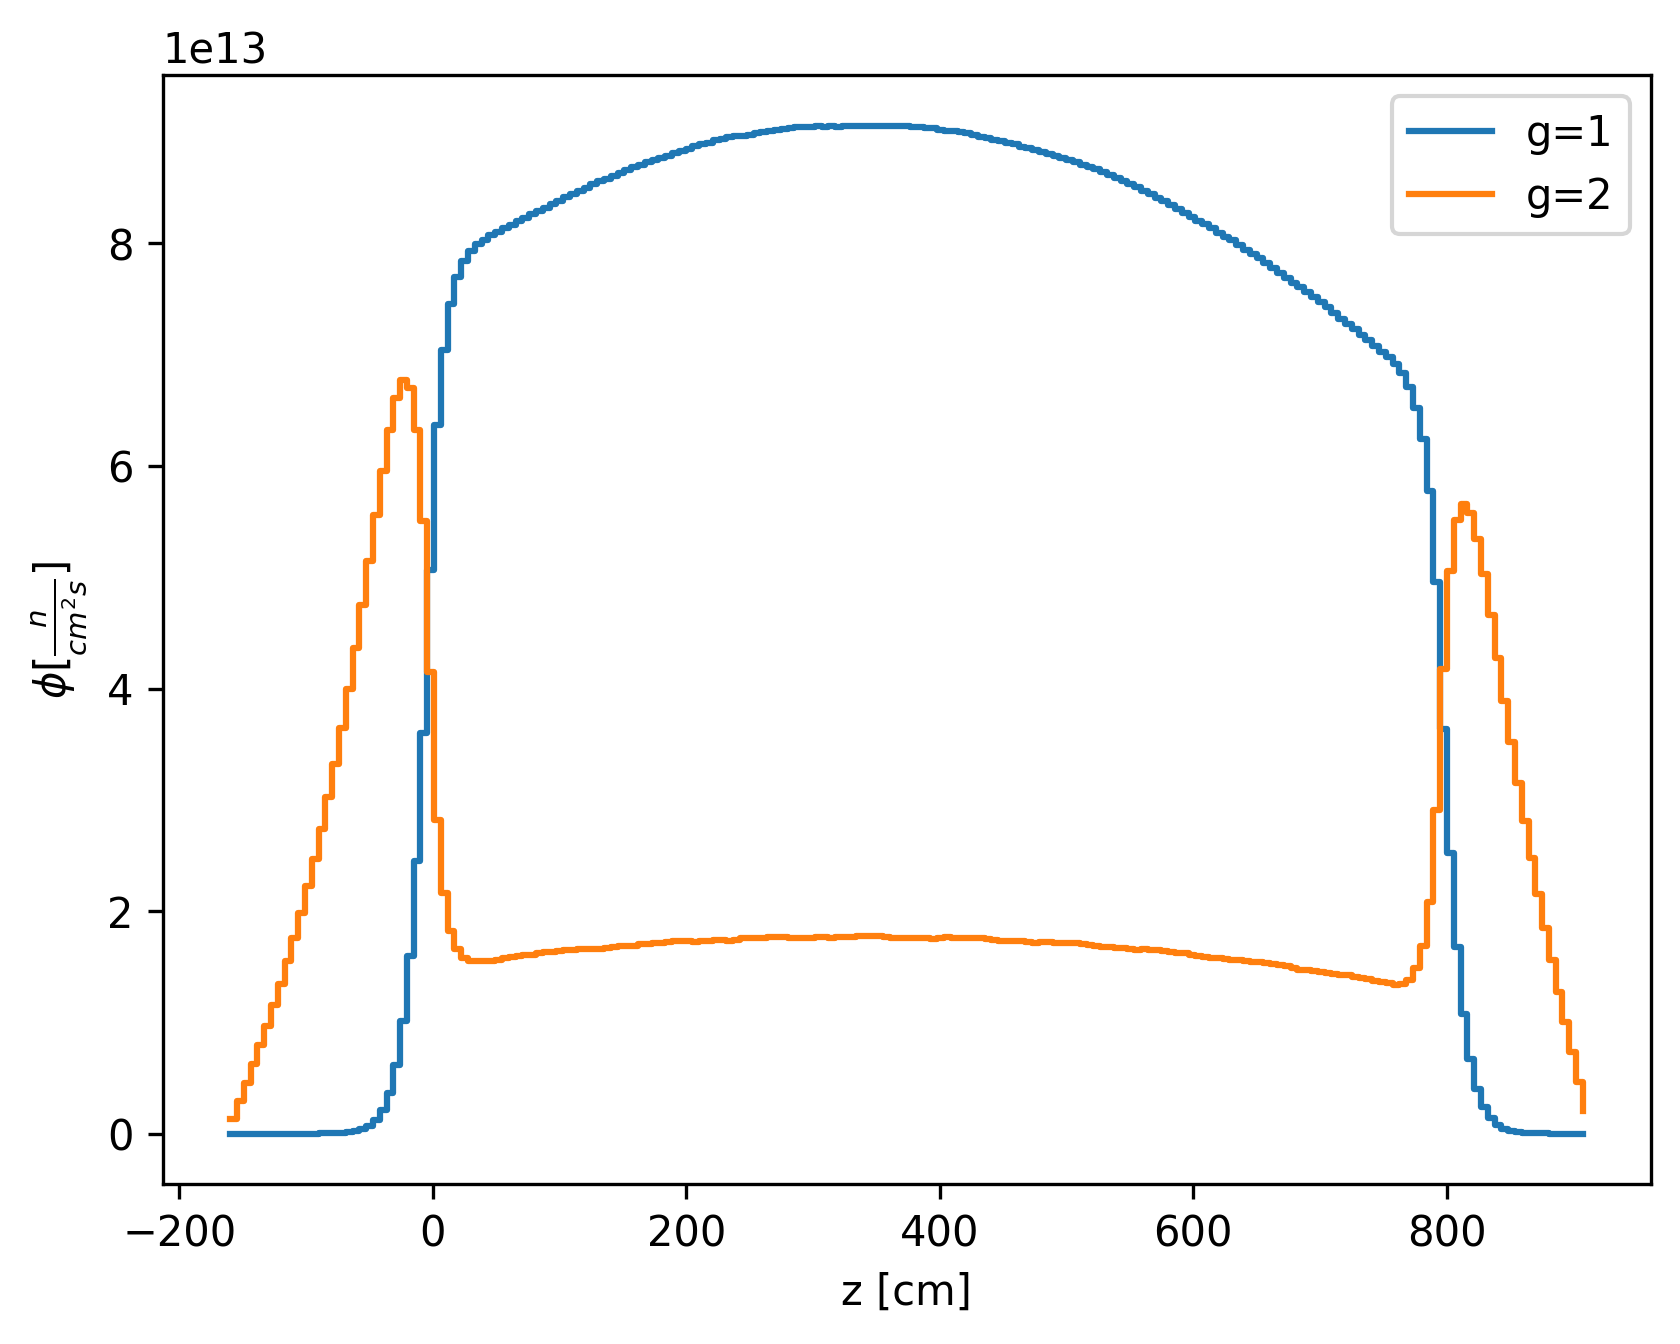
\includegraphics[width=0.45\textwidth]{figures-neutronics/standard-column-detector-Axial}
    }
    \subfloat[Moltres axial flux.]{
        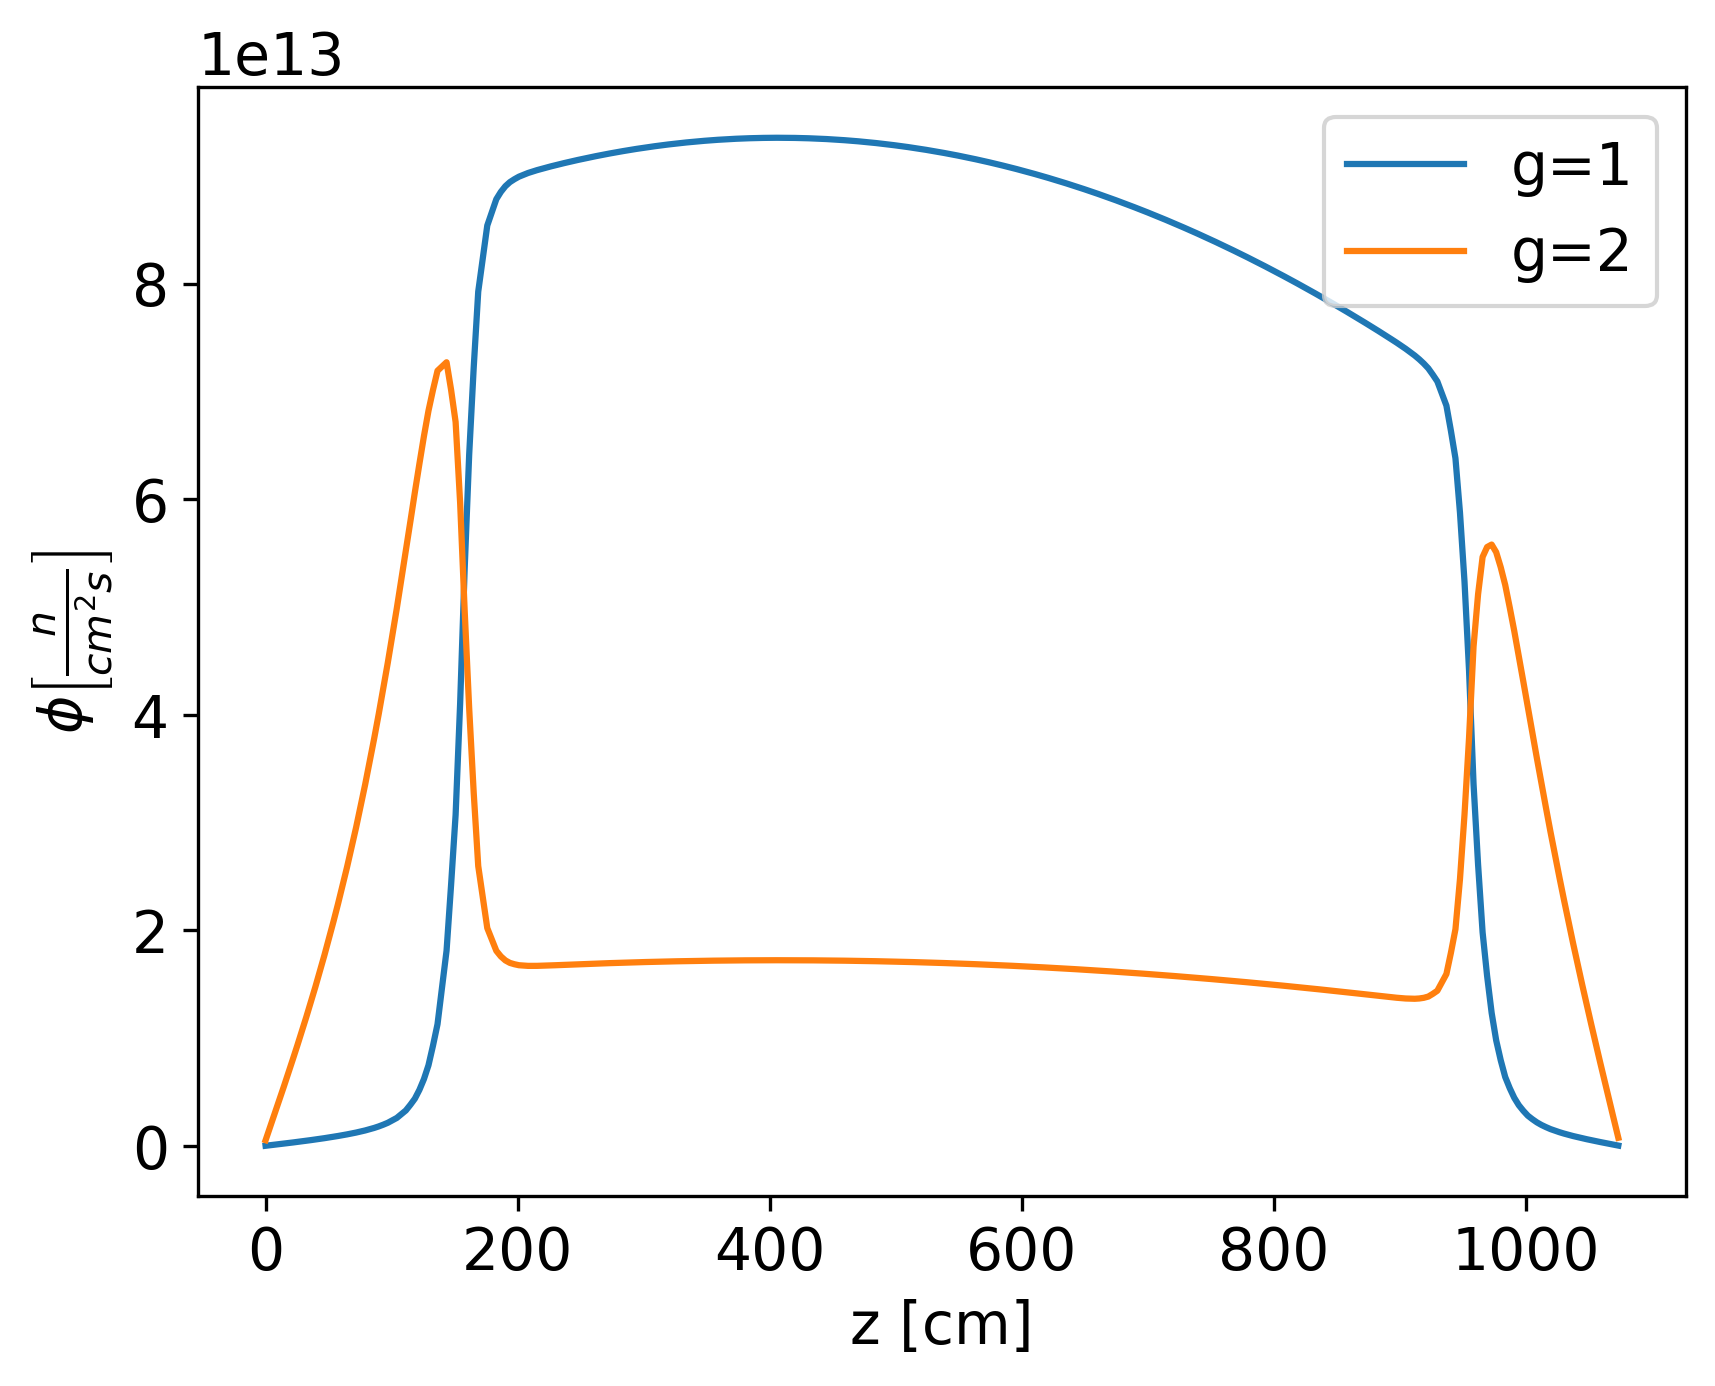
\includegraphics[width=0.45\textwidth]{figures-neutronics/standard-column-homo}
    }
	\hfill
  \caption{Two energy group axial flux in the fuel column calculated with Serpent and Moltres.}
	\label{fig:prelim}
\end{figure}

\section{Serpent-Moltres comparison}
\label{sec:neut-serpent}

In this section, Serpent modeled a fuel column and the full-core of the MHTGR-350.
Serpent obtained the homogenized group constants that served as input to Moltres.
The following sections compare Moltres and Serpent results as a validation exercise.
This exercise demonstrates that Moltres results are comparable to Serpent results, proving that Moltres diffusion solver is applicable to prismatic HTGRs and that Moltres can handle Serpent generated group constants for obtaining the diffusion solution.

\subsection{Fuel column}
\label{sec:neut-fuelcol}

This section investigates the effects of the energy group structure on the diffusion simulations.
The first analysis varied the number of energy groups, while a second analysis varied the energy group structures with a constant number of energy groups.
To reduce the computational expense, the analyses focused on a fuel column of the MHTGR-350, shown in Figure \ref{fig:fuelcolumn}.
% The fuel column includes the bottom and top reflectors.
Tables \ref{tab:element-characteristics} and \ref{tab:compact} specify the model input parameters.

The first step in the calculation obtained the group constants using Serpent.
For simplicity, Serpent's model did not consider the fuel handling holes or the bottom and top reflectors' coolant channels.
HTGRs use burnable poisons to reduce the power peaking factors in various active core regions.
Some reactors have burnable poisons in the rings closer to the reflectors and no burnable poisons in the middle rings.
This characteristic motivated the analysis of two cases: one fuel column that does not have burnable poisons and one that does.
The burnable poisons' locations are the six corners of the fuel assembly, shown in Figure \ref{fig:fuelassembly}.
The material temperatures were 600 and 1200K, cases that represent the \gls{CZP} and the \gls{HFP} core states \cite{strydom_results_2015}.
The Serpent simulations included 4$\times 10^5$ neutrons/cycle, 360 active cycles, and 40 inactive cycles for the calculations.

Taking advantage of the problem's symmetry, Moltres modeled a $1/12^{th}$-section of the homogenized fuel column.
The mesh had 3.71 $\times 10^4$ elements and 2.29 $\times 10^4$ nodes.
The diffusion calculations had 2.29 $\times 10^4$ \glspl{DoF} per energy-group.
The Moltres input files set an eigenvalue and a flux convergence tolerance of 10$^{-8}$.
Moltres calculations used the different energy group structures listed in Table \ref{tab:energygroups}.

\begin{table}[htbp!]
  \centering
  \caption{Energy group structure \cite{iaea_evaluation_2003}.}
  \begin{tabular}{S[table-format=2.2e-1]|llllllllllll}
  \toprule
                      & \multicolumn{12}{c}{Group structure} \\
  \multicolumn{1}{c|}{Upper boundary [eV]} & 26    & 21   & 18   & 15a & 15b & 15c & 15d & 15e   & 12  & 9  & 6  & 3 \\
  \midrule
  1.49e+07            & 1     & 1    & 1    & 1   & 1   & 1   & 1   & 1     & 1   & 1  & 1  & 1 \\ 
  7.41e+06            & 2     &      &      &     &     &     &     &       &     &    &    &   \\ 
  3.68e+06            & 3     & 2    & 2    & 2   & 2   & 2   & 2   & 2     & 2   &    &    &   \\ 
  6.72e+05            & 4     &      &      &     &     &     &     &       &     &    &    &   \\ 
  1.11e+05            & 5     & 3    & 3    & 3   & 3   & 3   & 3   & 3     & 3   & 2  & 2  & 2 \\ 
  1.93e+04            & 6     & 4    & 4    & 4   & 4   &     &     &       & 4   &    &    &   \\ 
  3.35e+03            & 7     &      &      &     &     &     &     &       &     &    &    &   \\ 
  1.58e+03            & 8     & 5    & 5    &     &     & 4   &     &       &     &    &    &   \\ 
  7.48e+02            & 9     & 6    & 6    & 5   & 5   &     & 4   & 4     & 5   & 3  &    &   \\ 
  2.75e+02            & 10    & 7    & 7    & 6   & 6   & 5   &     &       & 6   & 4  &    &   \\ 
  1.30e+02            & 11    & 8    & 8    & 7   & 7   &     & 5   & 5     & 7   & 5  & 3  &   \\ 
  6.14e+01            & 12    & 9    &      &     & 8   & 6   &     &       &     &    &    &   \\ 
  2.90e+01            & 13    & 10   & 9    & 8   & 9   &     & 6   & 6     &     &    &    &   \\ 
  1.37e+01            & 14    & 11   & 10   & 9   &     &     &     &       & 8   & 6  &    &   \\ 
  8.32e+00            & 15    & 12   & 11   & 10  & 10  & 7   & 7   & 7     & 9   &    &    &   \\ 
  5.04e+00            & 16    &      &      &     &     &     &     &       &     &    &    &   \\ 
  2.38e+00            & 17    & 13   & 12   & 11  & 11  & 8   & 8   & 8     & 10  & 7  & 4  & 3 \\ 
  1.29e+00            & 18    & 14   &      &     &     &     &     &       &     &    &    &   \\ 
  6.50e-01            & 19    & 15   & 13   & 12  & 12  & 9   & 9   & 9     & 11  & 8  & 5  &   \\ 
  3.50e-01            & 20    & 16   &      &     &     & 10  & 10  &       &     &    &    &   \\ 
  2.00e-01            & 21    & 17   & 14   & 13  & 13  & 11  & 11  & 10    &     &    &    &   \\ 
  1.20e-01            & 22    &      &      &     &     &     &     & 11    &     &    &    &   \\ 
  8.00e-02            & 23    & 18   & 15   & 14  & 14  & 12  & 12  & 12    &     &    &    &   \\ 
  5.00e-02            & 24    & 19   & 16   &     &     & 13  & 13  & 13    &     &    &    &   \\ 
  2.00e-02            & 25    & 20   & 17   & 15  & 15  & 14  & 14  & 14    & 12  & 9  & 6  &   \\ 
  1.00e-02            & 26    & 21   & 18   &     &     & 15  & 15  & 15    &     &    &    &   \\ 
  \bottomrule
  \end{tabular}
  \label{tab:energygroups}
\end{table}

% Fluxes
Summarizing, the analyses included four operational cases: 
\begin{itemize}
  \item Operational case 1: fuel column with no burnable poisons at 600K.
  \item Operational case 2: fuel column with no burnable poisons at 1200K.
  \item Operational case 3: fuel column with burnable poisons at 600K.
  \item Operational case 4: fuel column with burnable poisons at 1200K.
\end{itemize}

% This is very important and I should review it carefully
To compare the results from Serpent and Moltres, we compare the axial flux.
Moltres ran the calculations using 26 energy groups.
The results present the axial fluxes collapsed into three energy groups to facilitate the results' visualization.
Figures \ref{fig:assembly-noLBP-600-flux} to \ref{fig:assembly-LBP-1200-flux} display the axial flux from the Serpent and the Moltres simulations for all cases.
The figures also display the relative difference between Serpent and Moltres results calculated as follows
\begin{align}
  & \Delta = \frac{\phi_S-\phi_M}{\phi_S} \cdot 100  \label{eq:rel-error-flux}
  \intertext{where}
  & \Delta = \mbox{relative difference } [\%] \notag \\
  & \phi_S = \mbox{Serpent-calculated flux } [n \cdot cm^{-2} \cdot s^{-1}] \notag \\
  & \phi_M = \mbox{Moltres-calculated flux } [n \cdot cm^{-2} \cdot s^{-1}]. \notag
\end{align}

For all the operational cases, the fluxes from Serpent and Moltres look close in shape and magnitude.
For the operational case 1, 2, 3, and 4, the largest error is 98\%, 167\%, 99\%, and 1720\%, respectively.
The largest error occurs at the bottom reflector boundary.
This behavior is expected, as the diffusion theory assumptions are weaker at boundaries.
Another spot where the diffusion theory assumptions are weaker is the interface between materials.
At the interfaces between the active core and reflectors, the largest error is 7\%, 8\%, 4\%, and 6\% for the operational case 1, 2, 3, and 4.
Focusing on the active core region only, the largest error is 1\%, 3\%, 4\%, and 6\% for the operational case 1, 2, 3, and 4.

% No LBP 600
\begin{figure}[htbp!]
	\centering
    \subfloat[Serpent and Moltres neutron fluxes.]{
        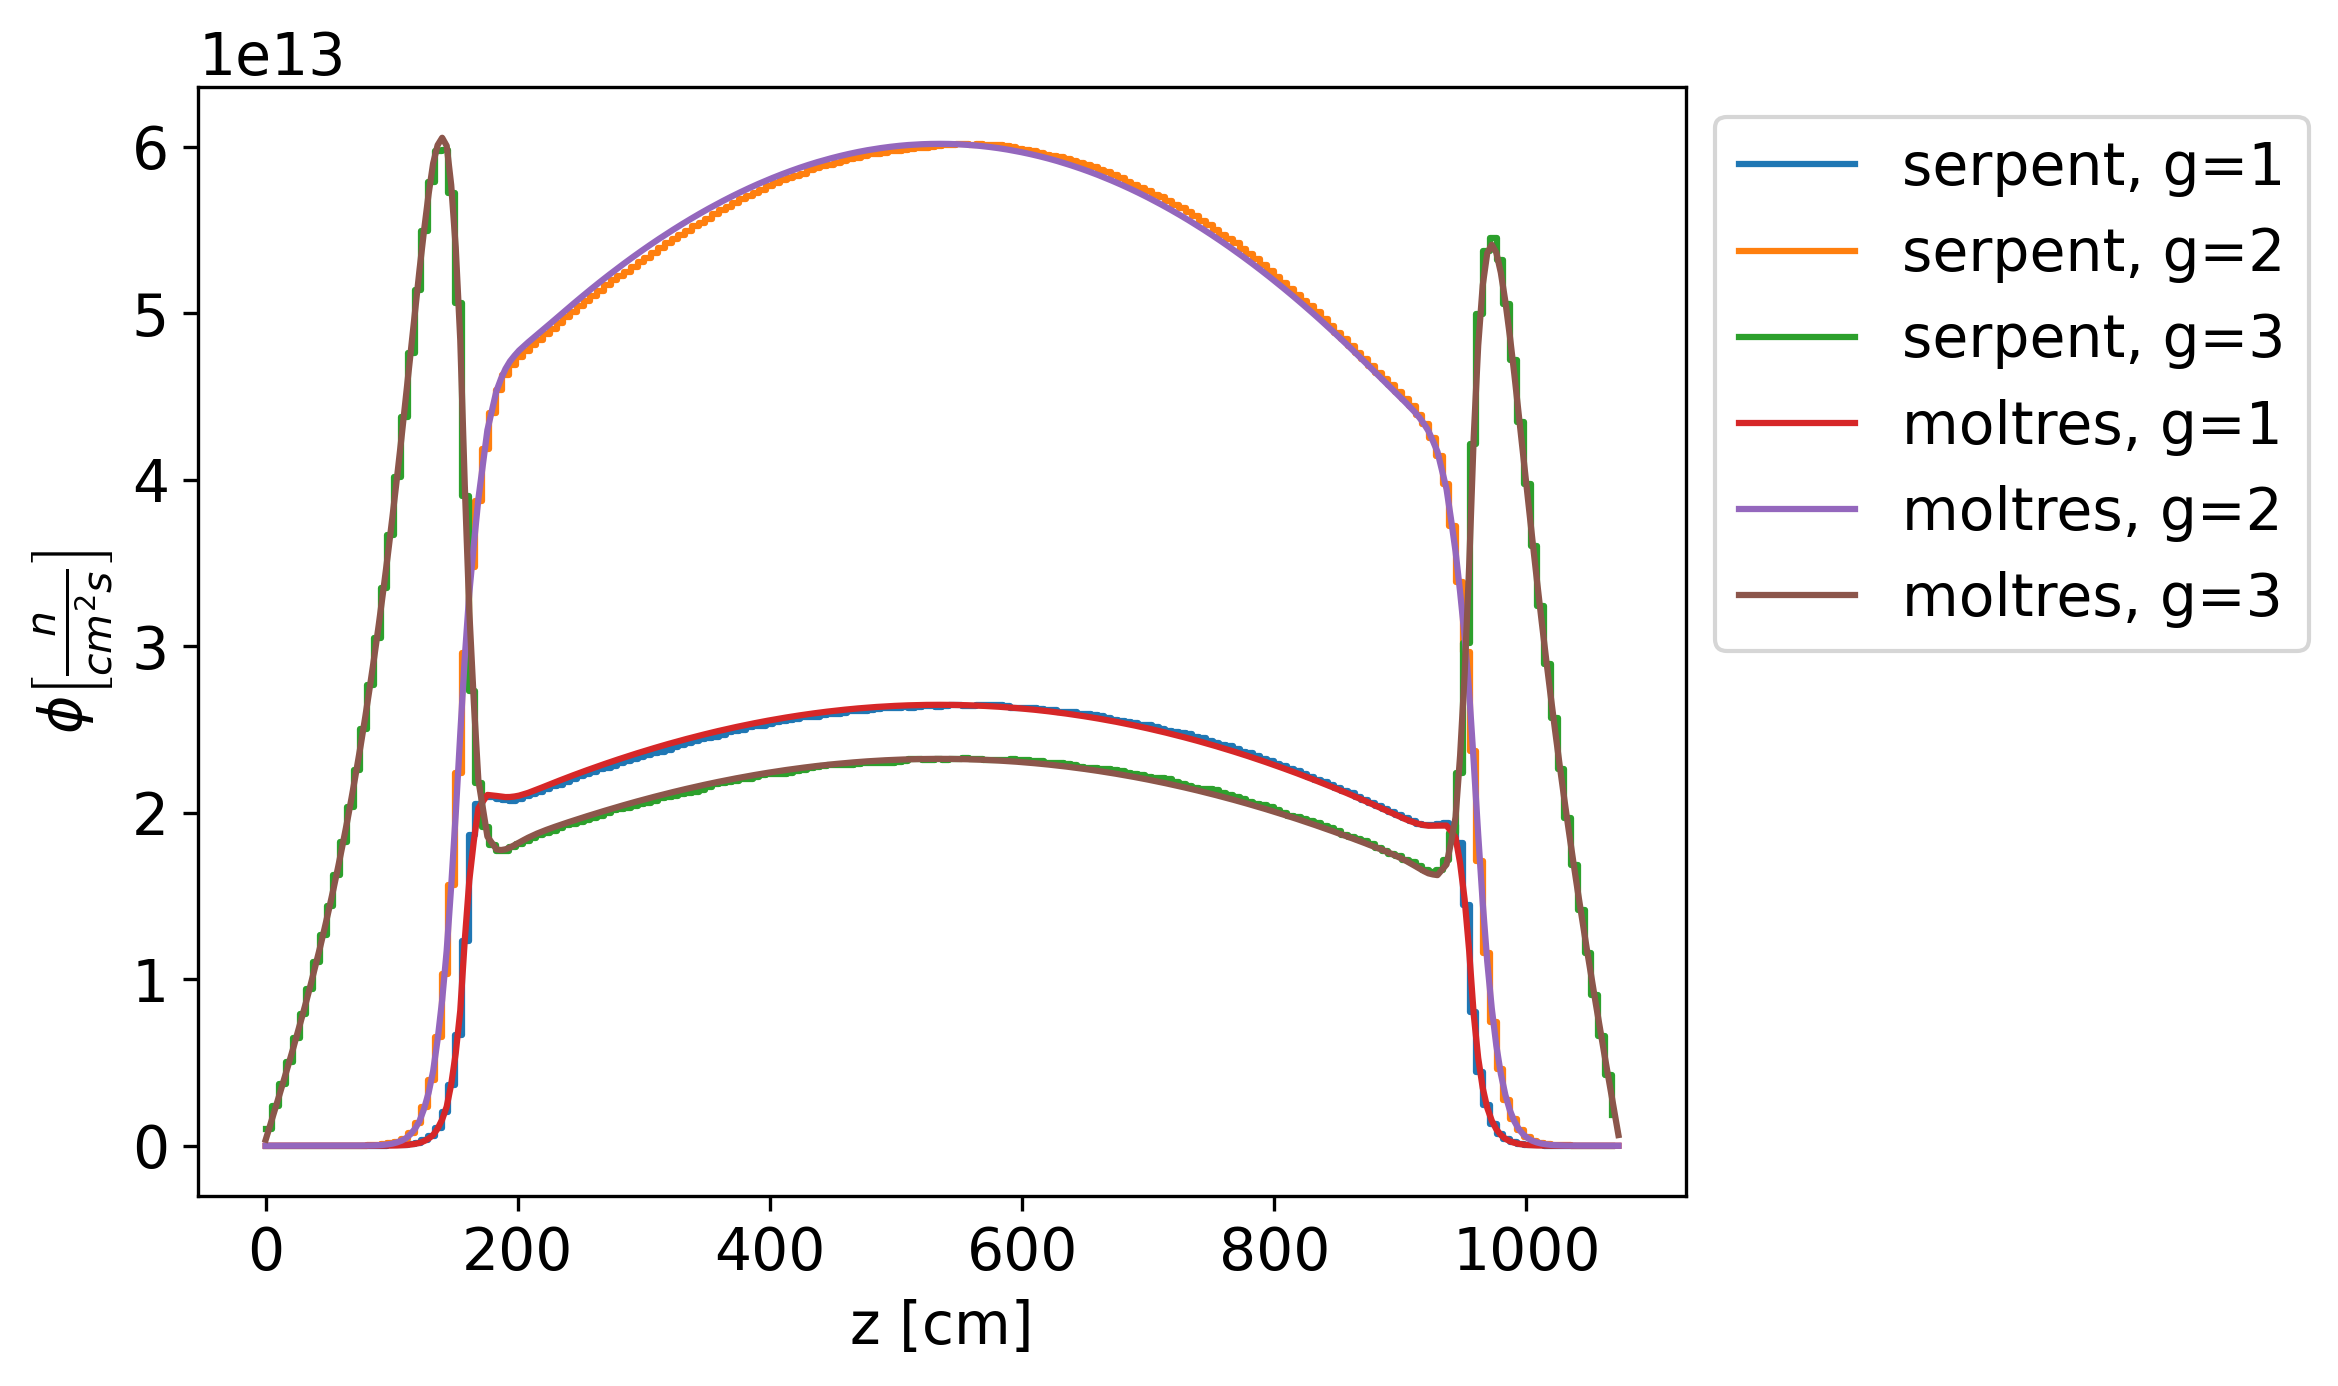
\includegraphics[width=0.51\textwidth]{figures-neutronics/serpent-moltres-noLBP-600-fluxes}
    }
    \subfloat[Relative difference between Serpent and Moltres neutron fluxes.]{
        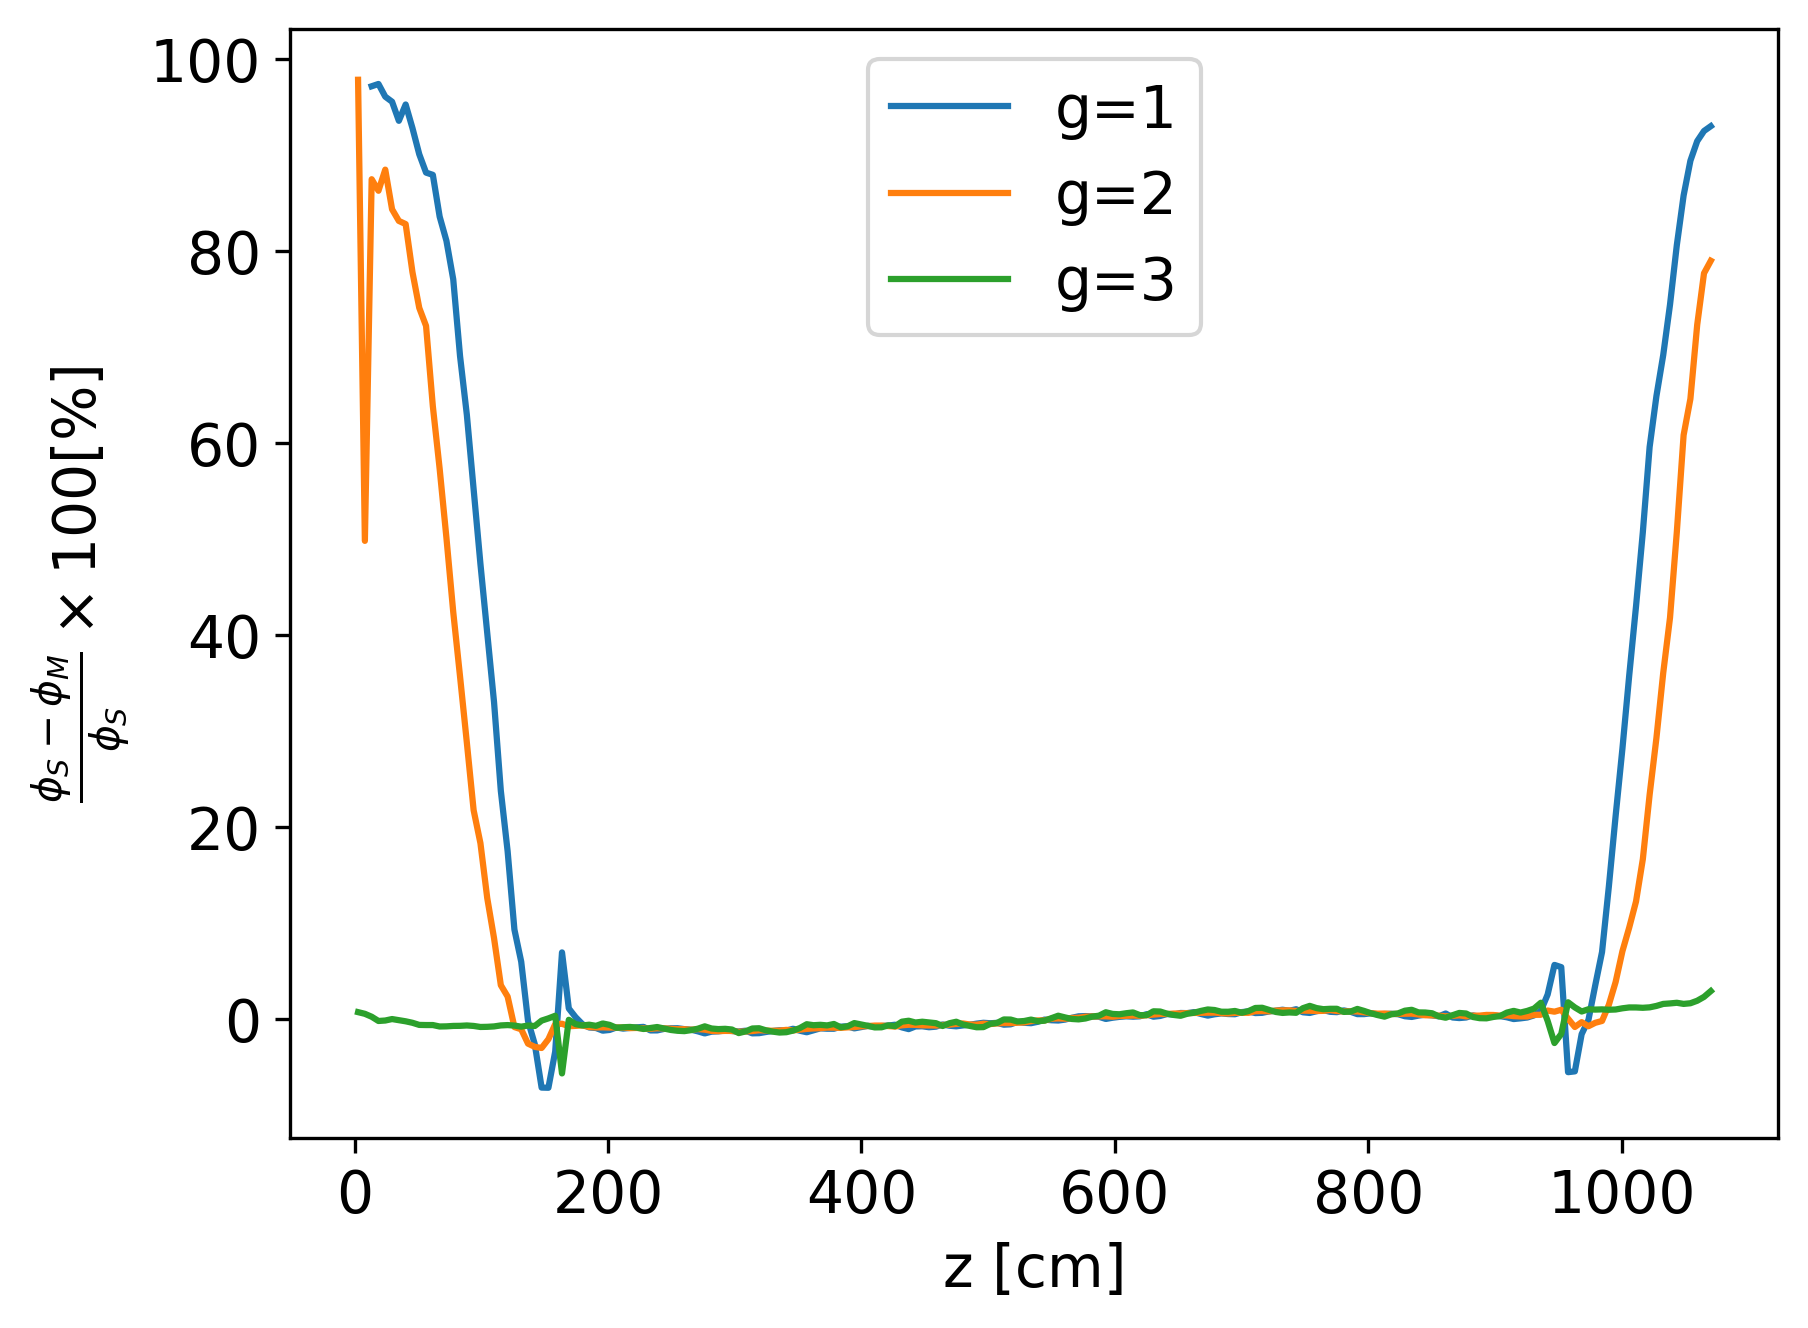
\includegraphics[width=0.39\textwidth]{figures-neutronics/serpent-moltres-noLBP-600-error}
    }
	\hfill
  \caption{Operational case 1: fuel column with no burnable poisons at 600K. Comparison of Serpent and Moltres-derived 3-group axial neutron fluxes.}
	\label{fig:assembly-noLBP-600-flux}
\end{figure}

% No LBP 1200
\begin{figure}[htbp!]
  \centering
    \subfloat[Serpent and Moltres neutron fluxes.]{
        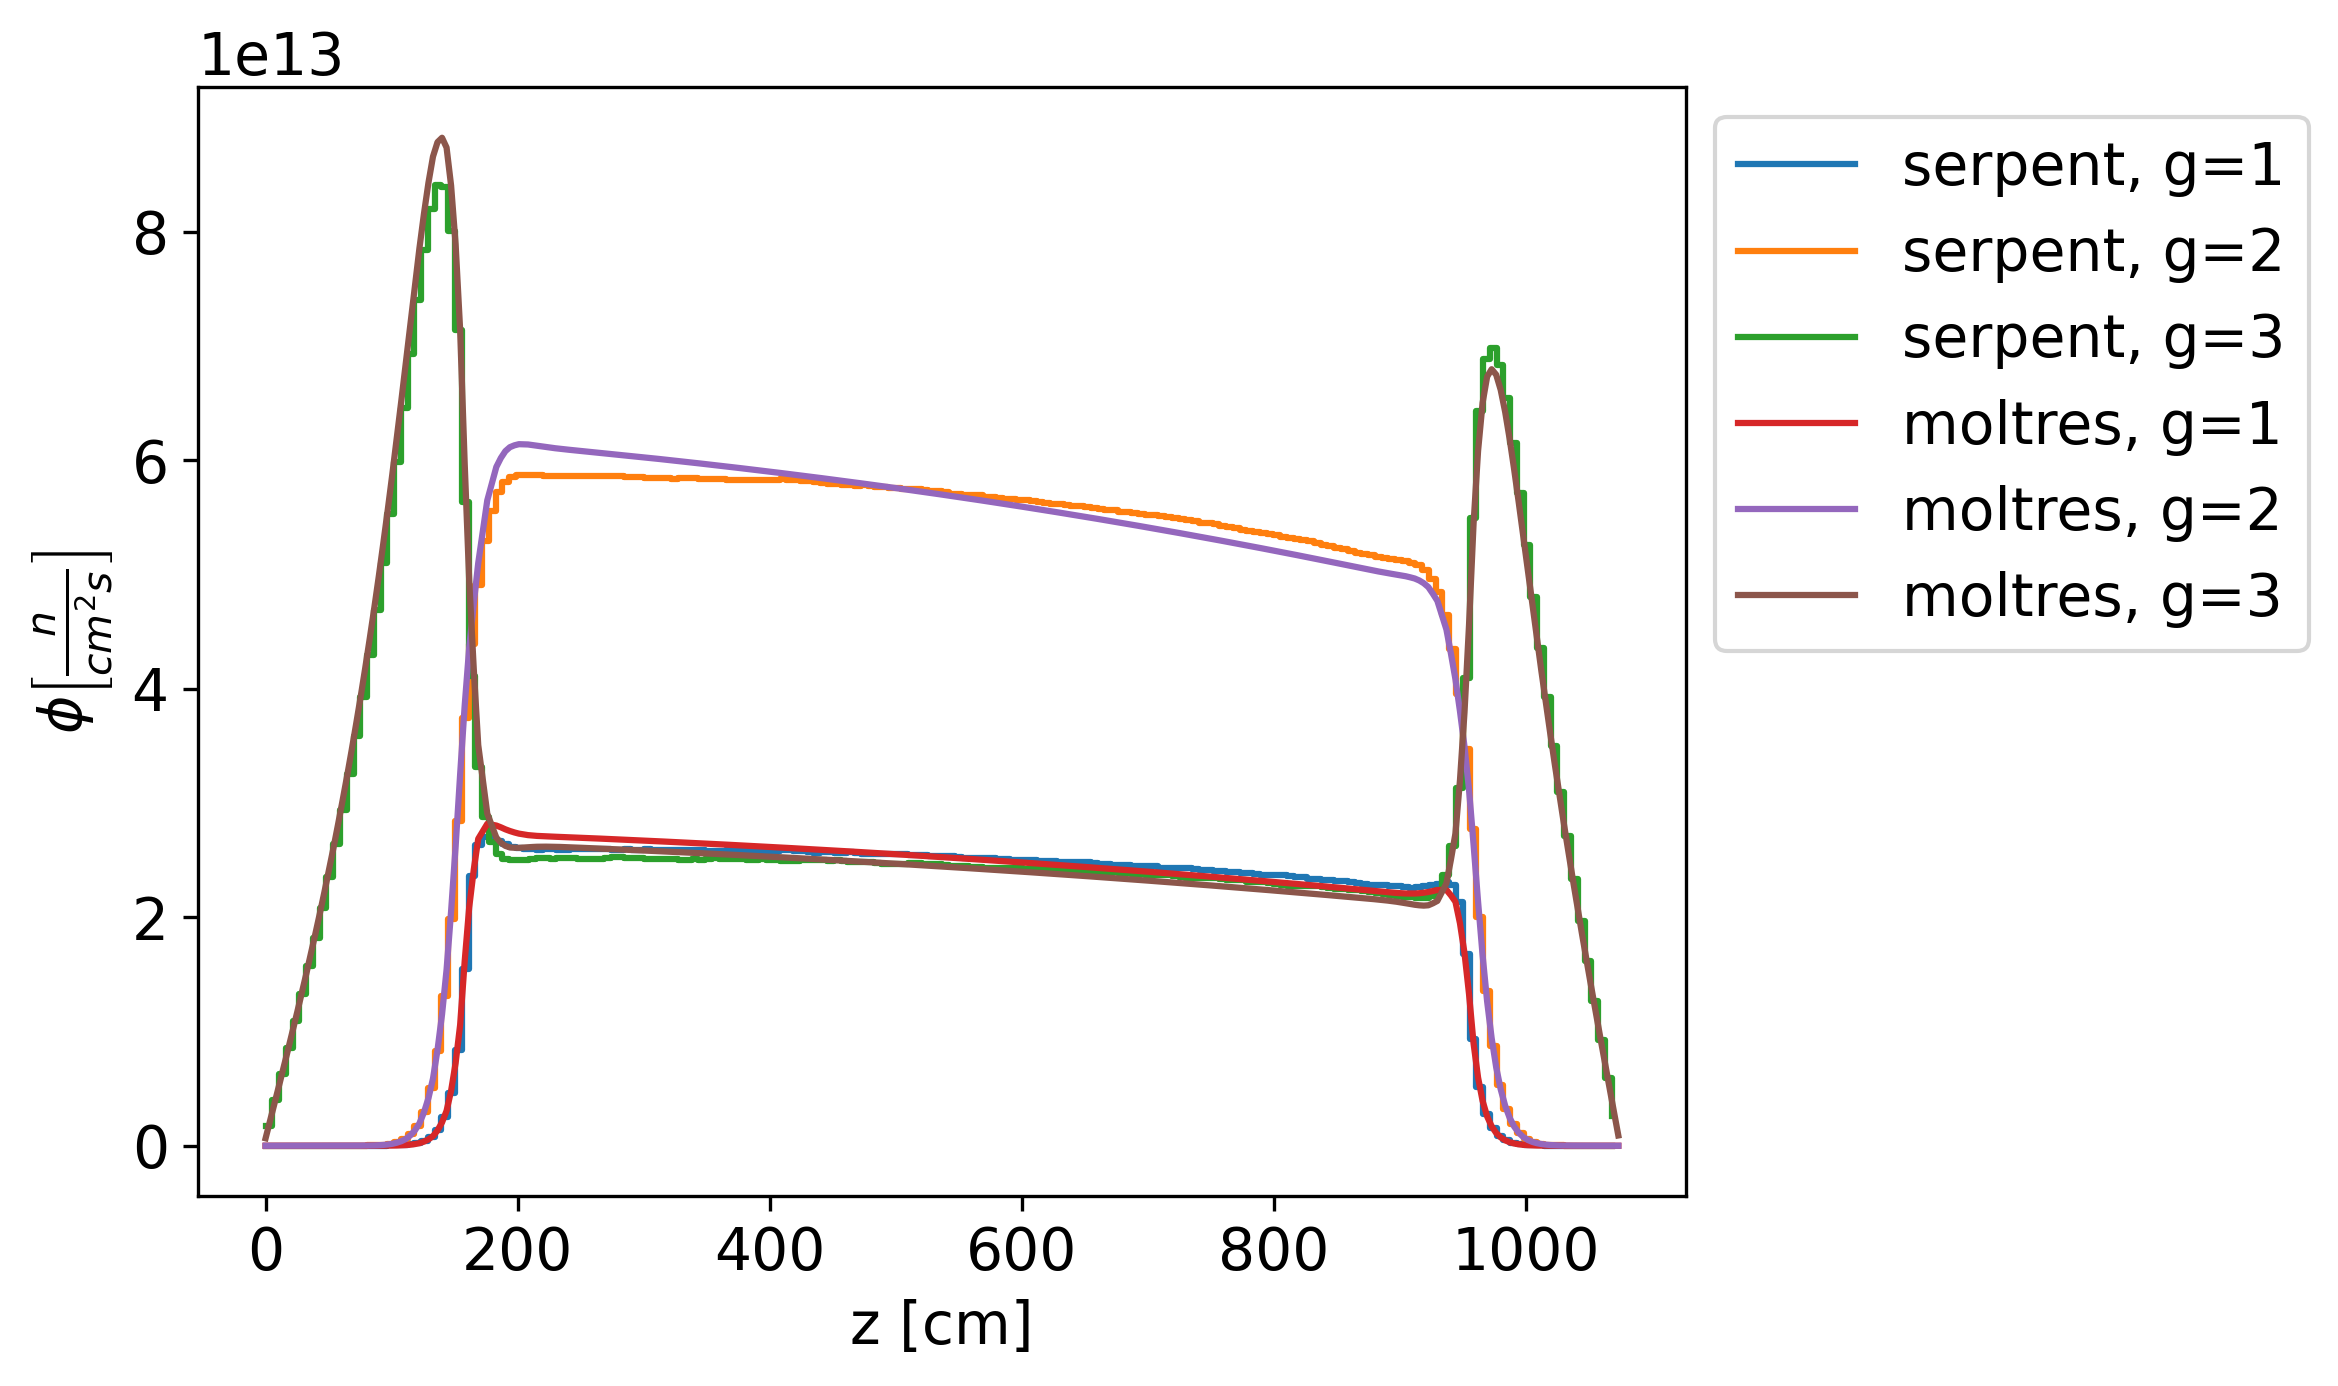
\includegraphics[width=0.51\textwidth]{figures-neutronics/serpent-moltres-noLBP-1200-fluxes}
    }
    \subfloat[Relative difference between Serpent and Moltres neutron fluxes.]{
        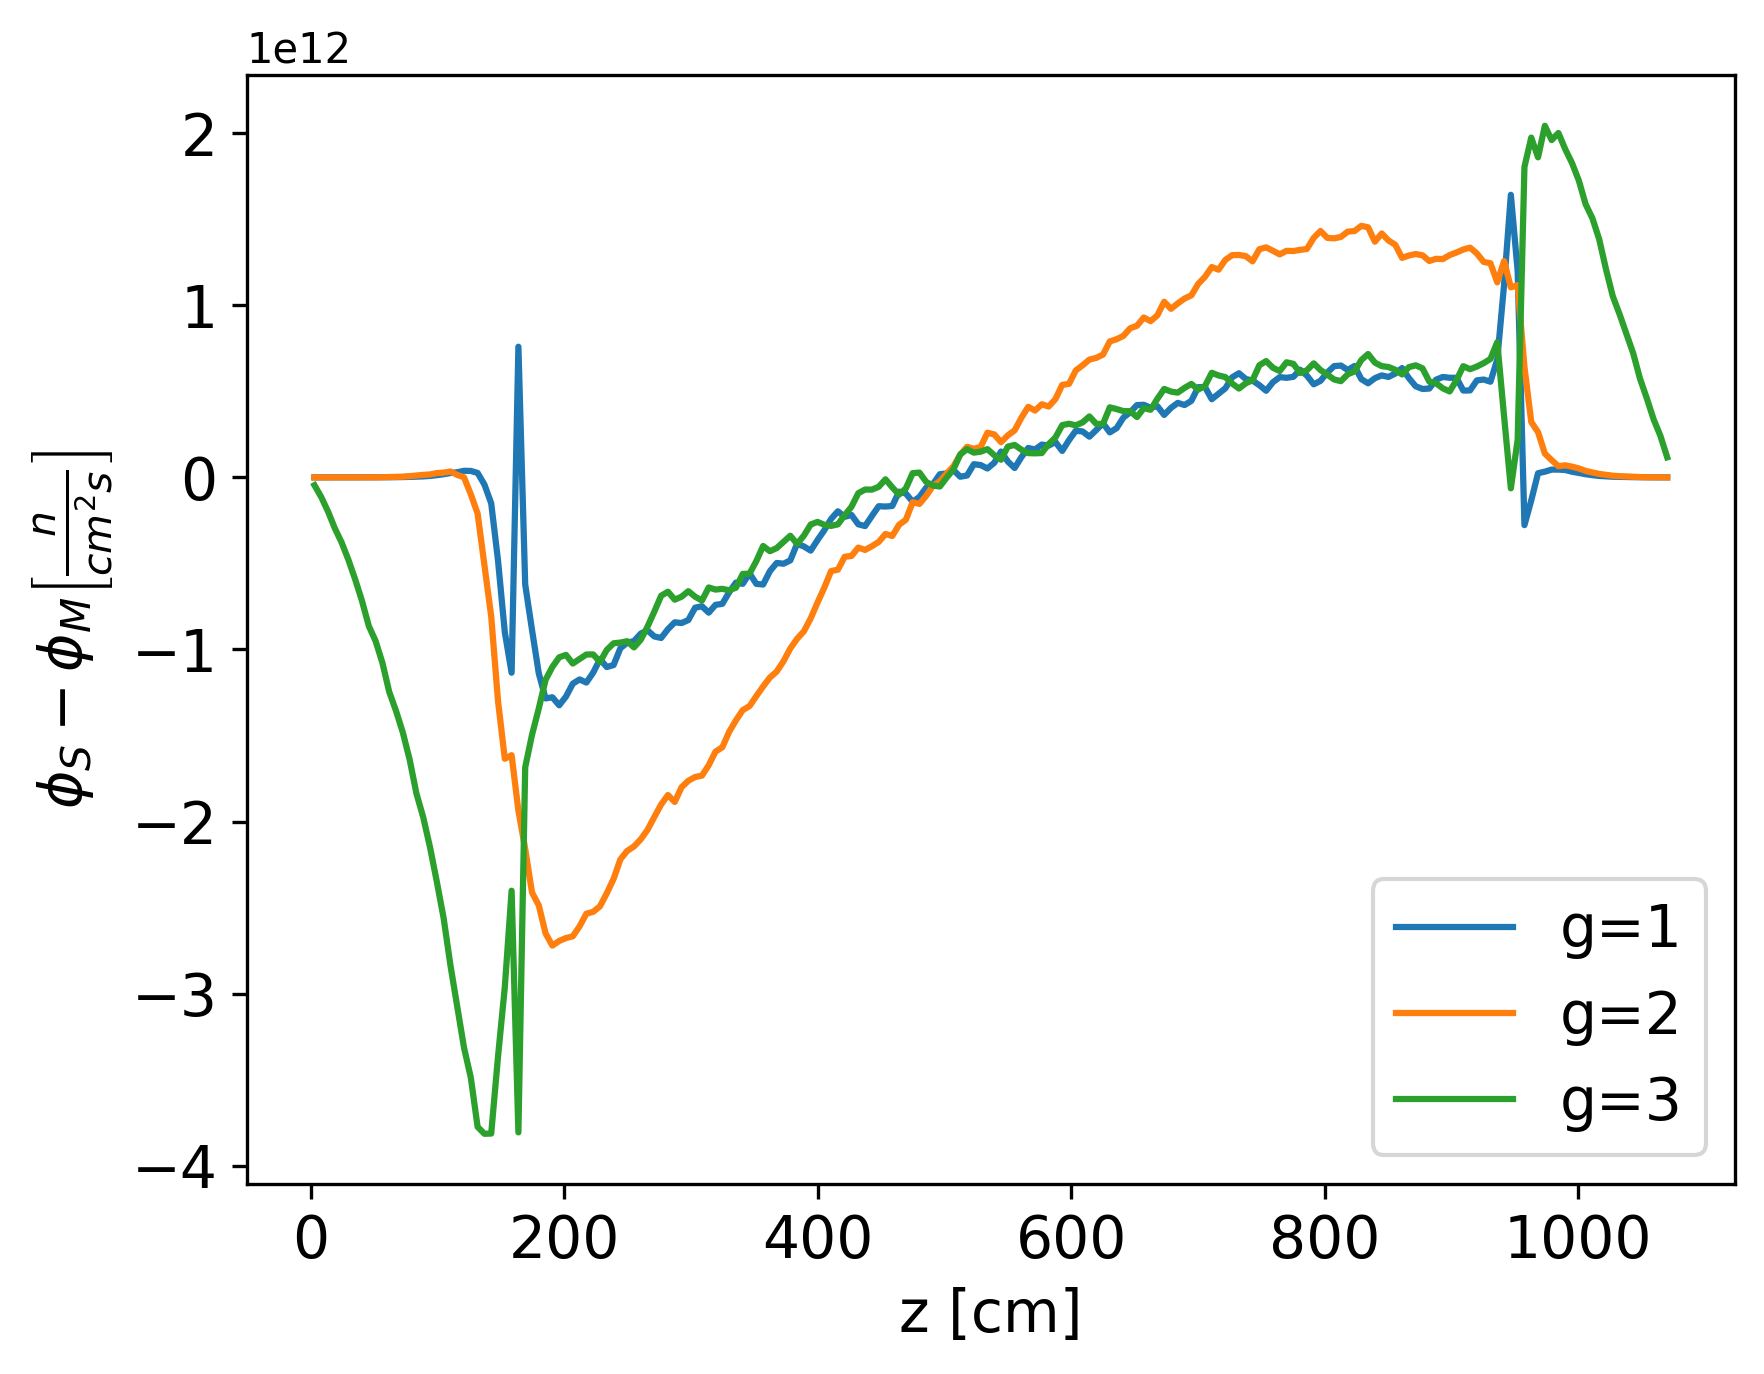
\includegraphics[width=0.39\textwidth]{figures-neutronics/serpent-moltres-noLBP-1200-error}
    }
  \hfill
  \caption{Operational case 2: fuel column with no burnable poisons at 1200K. Comparison of Serpent and Moltres-derived 3-group axial neutron fluxes.}
  \label{fig:assembly-noLBP-1200-flux}
\end{figure}

% LBP 600 
\begin{figure}[htbp!]
  \centering
    \subfloat[Serpent and Moltres neutron fluxes.]{
        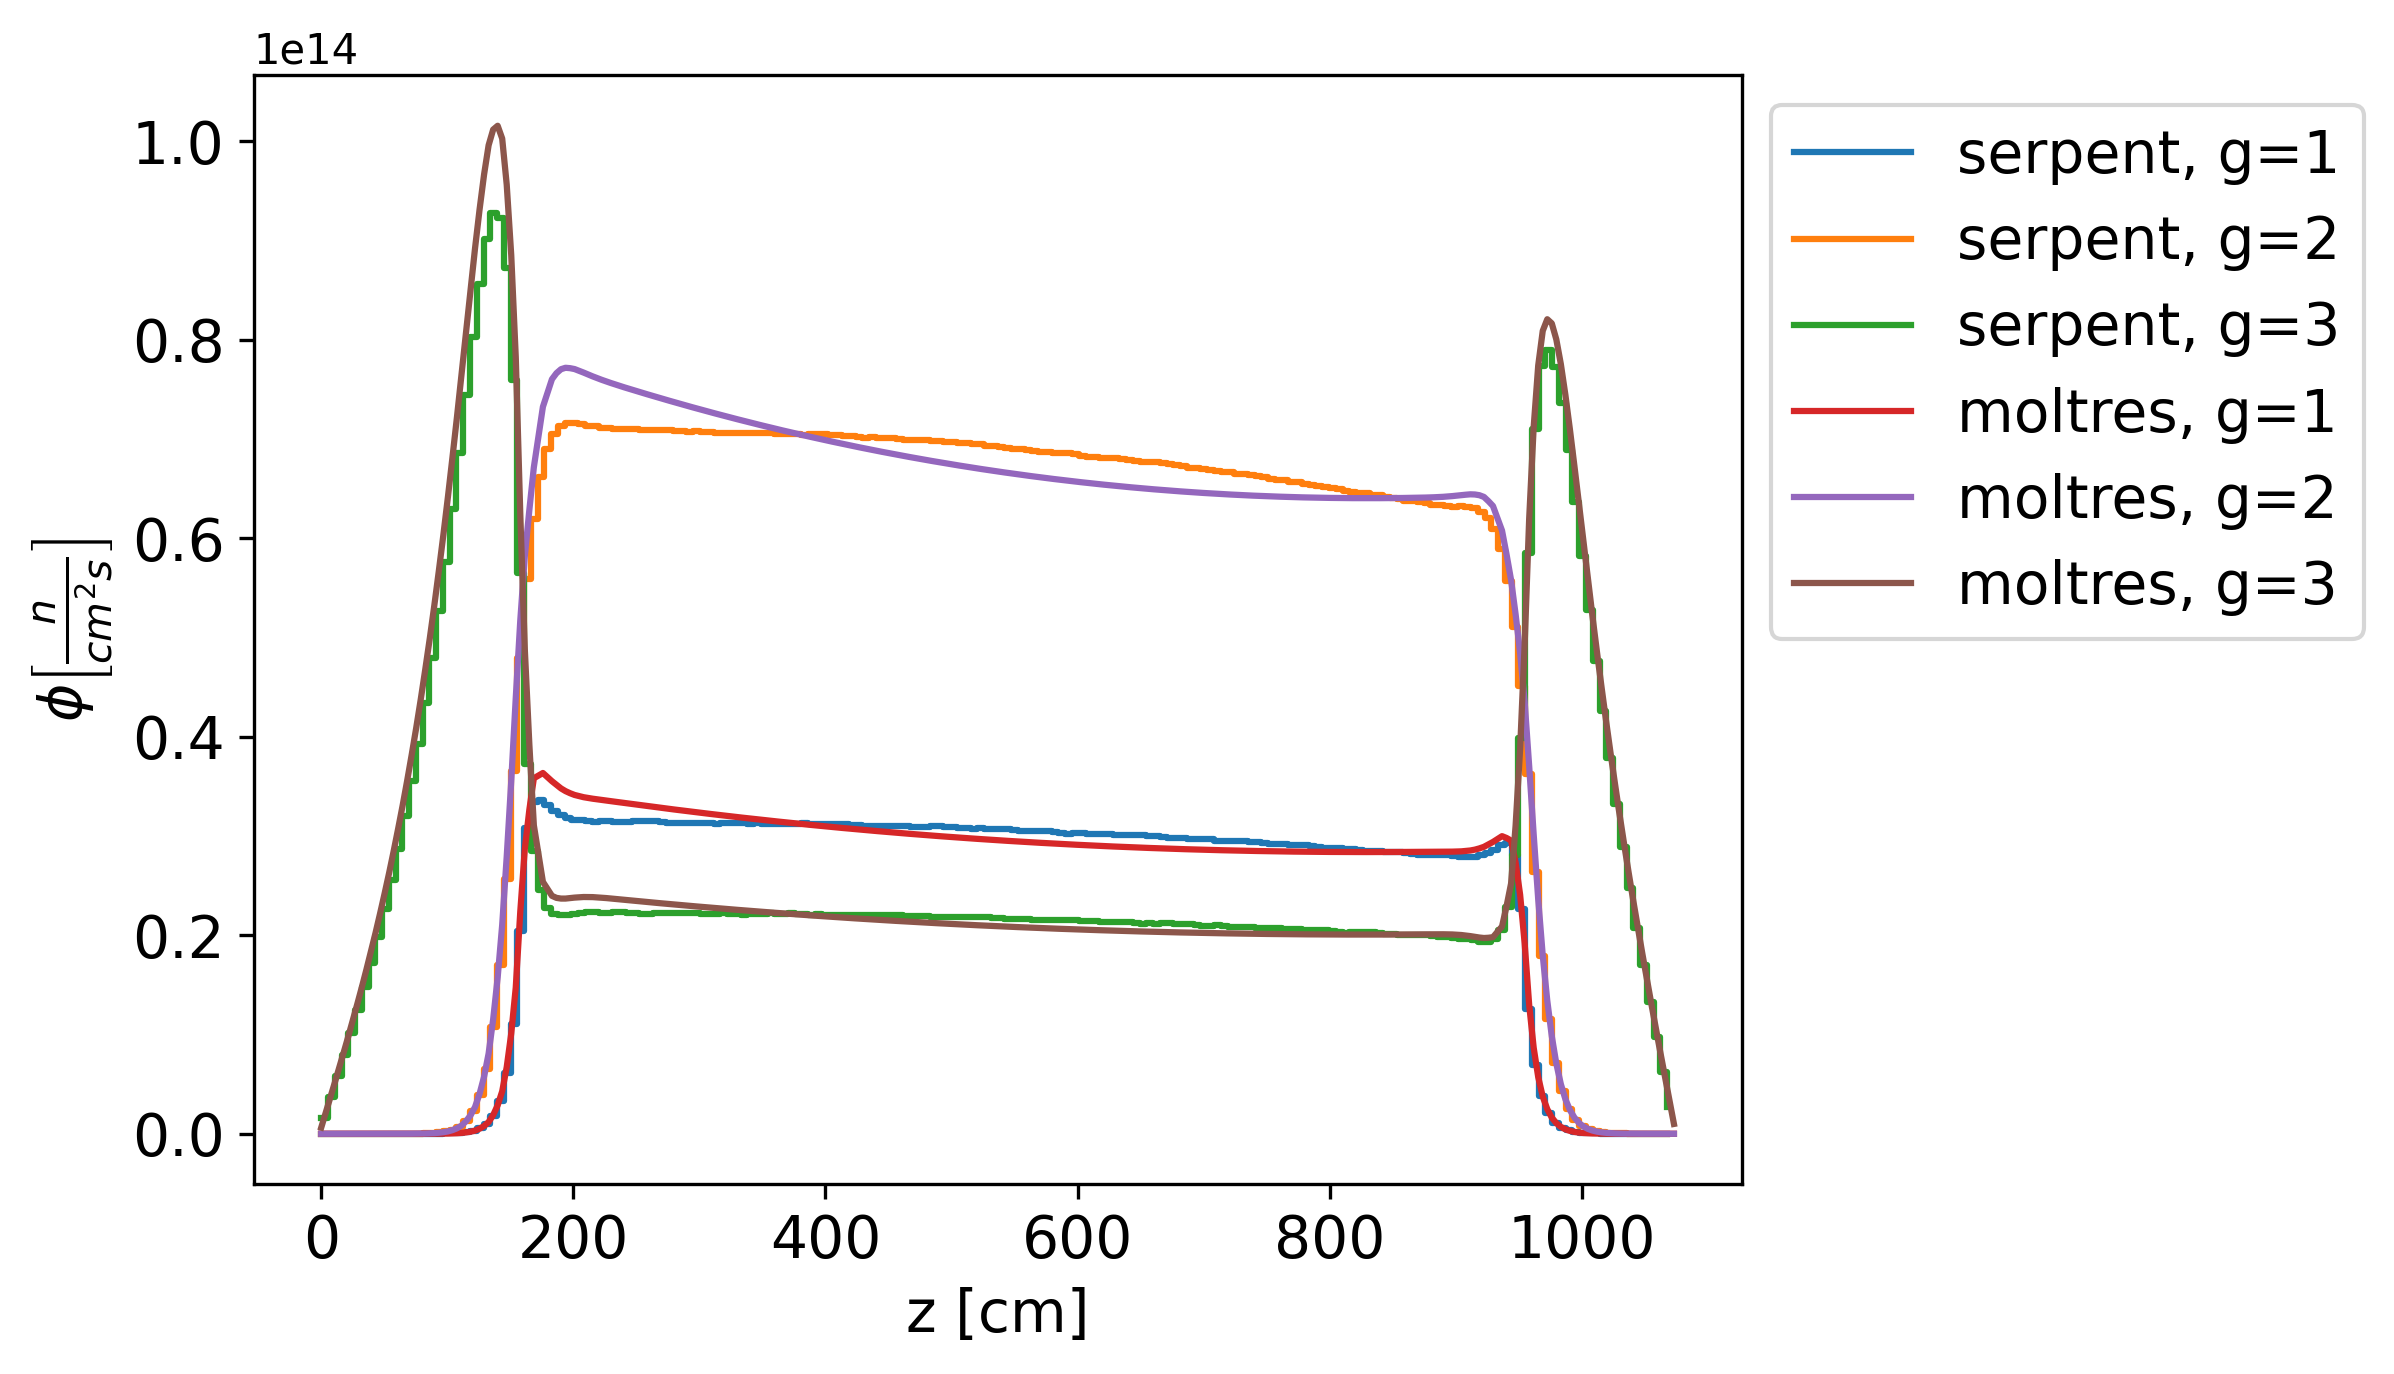
\includegraphics[width=0.51\textwidth]{figures-neutronics/serpent-moltres-LBP-600-fluxes}
    }
    \subfloat[Relative difference between Serpent and Moltres neutron fluxes.]{
        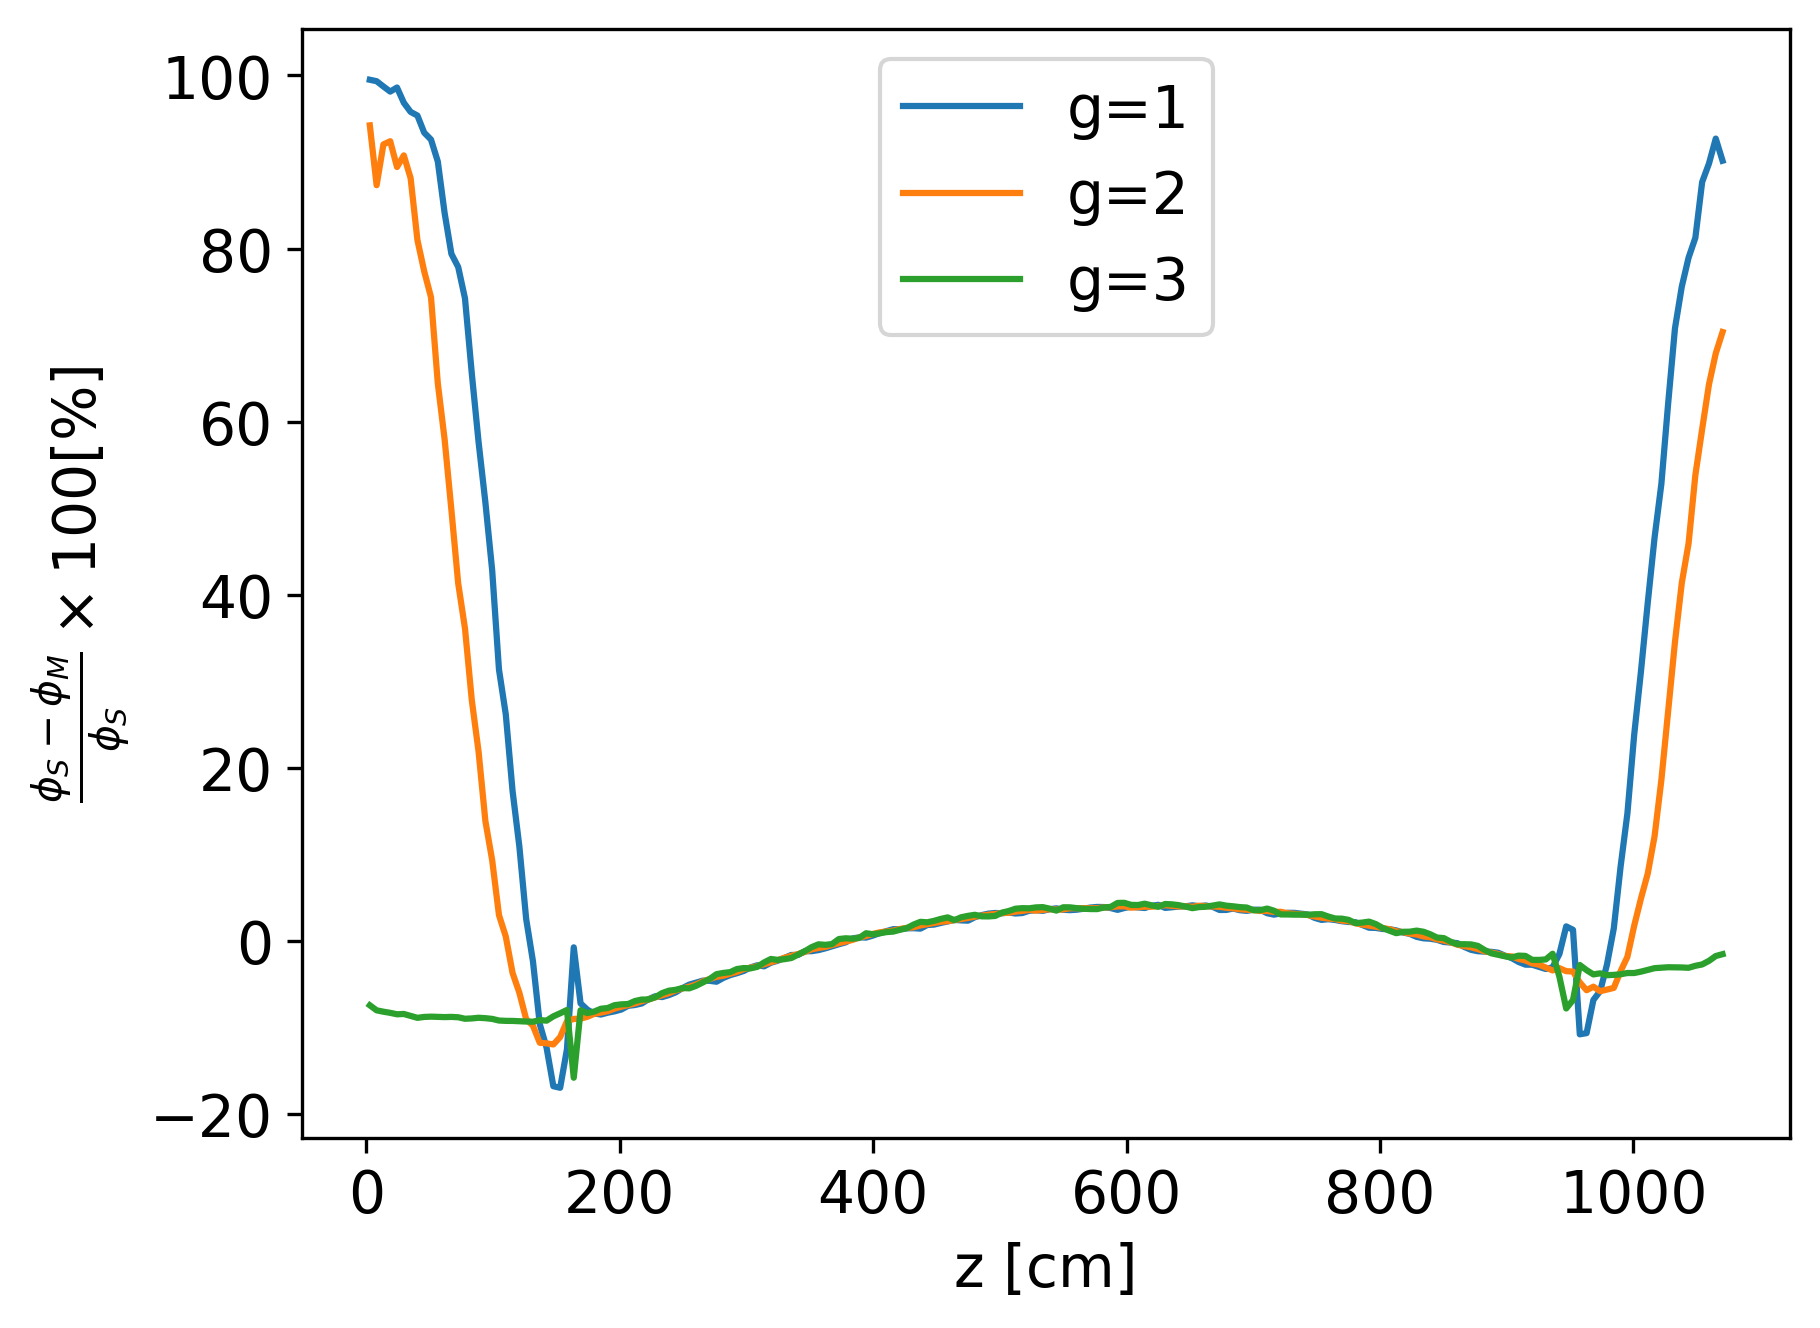
\includegraphics[width=0.39\textwidth]{figures-neutronics/serpent-moltres-LBP-600-error}
    }
  \hfill
  \caption{Operational case 3: fuel column with burnable poisons at 600K. Comparison of Serpent and Moltres-derived 3-group axial neutron fluxes.}
  \label{fig:assembly-LBP-600-flux}
\end{figure}

% LBP 1200
\begin{figure}[htbp!]
  \centering
    \subfloat[Serpent and Moltres neutron fluxes.]{
        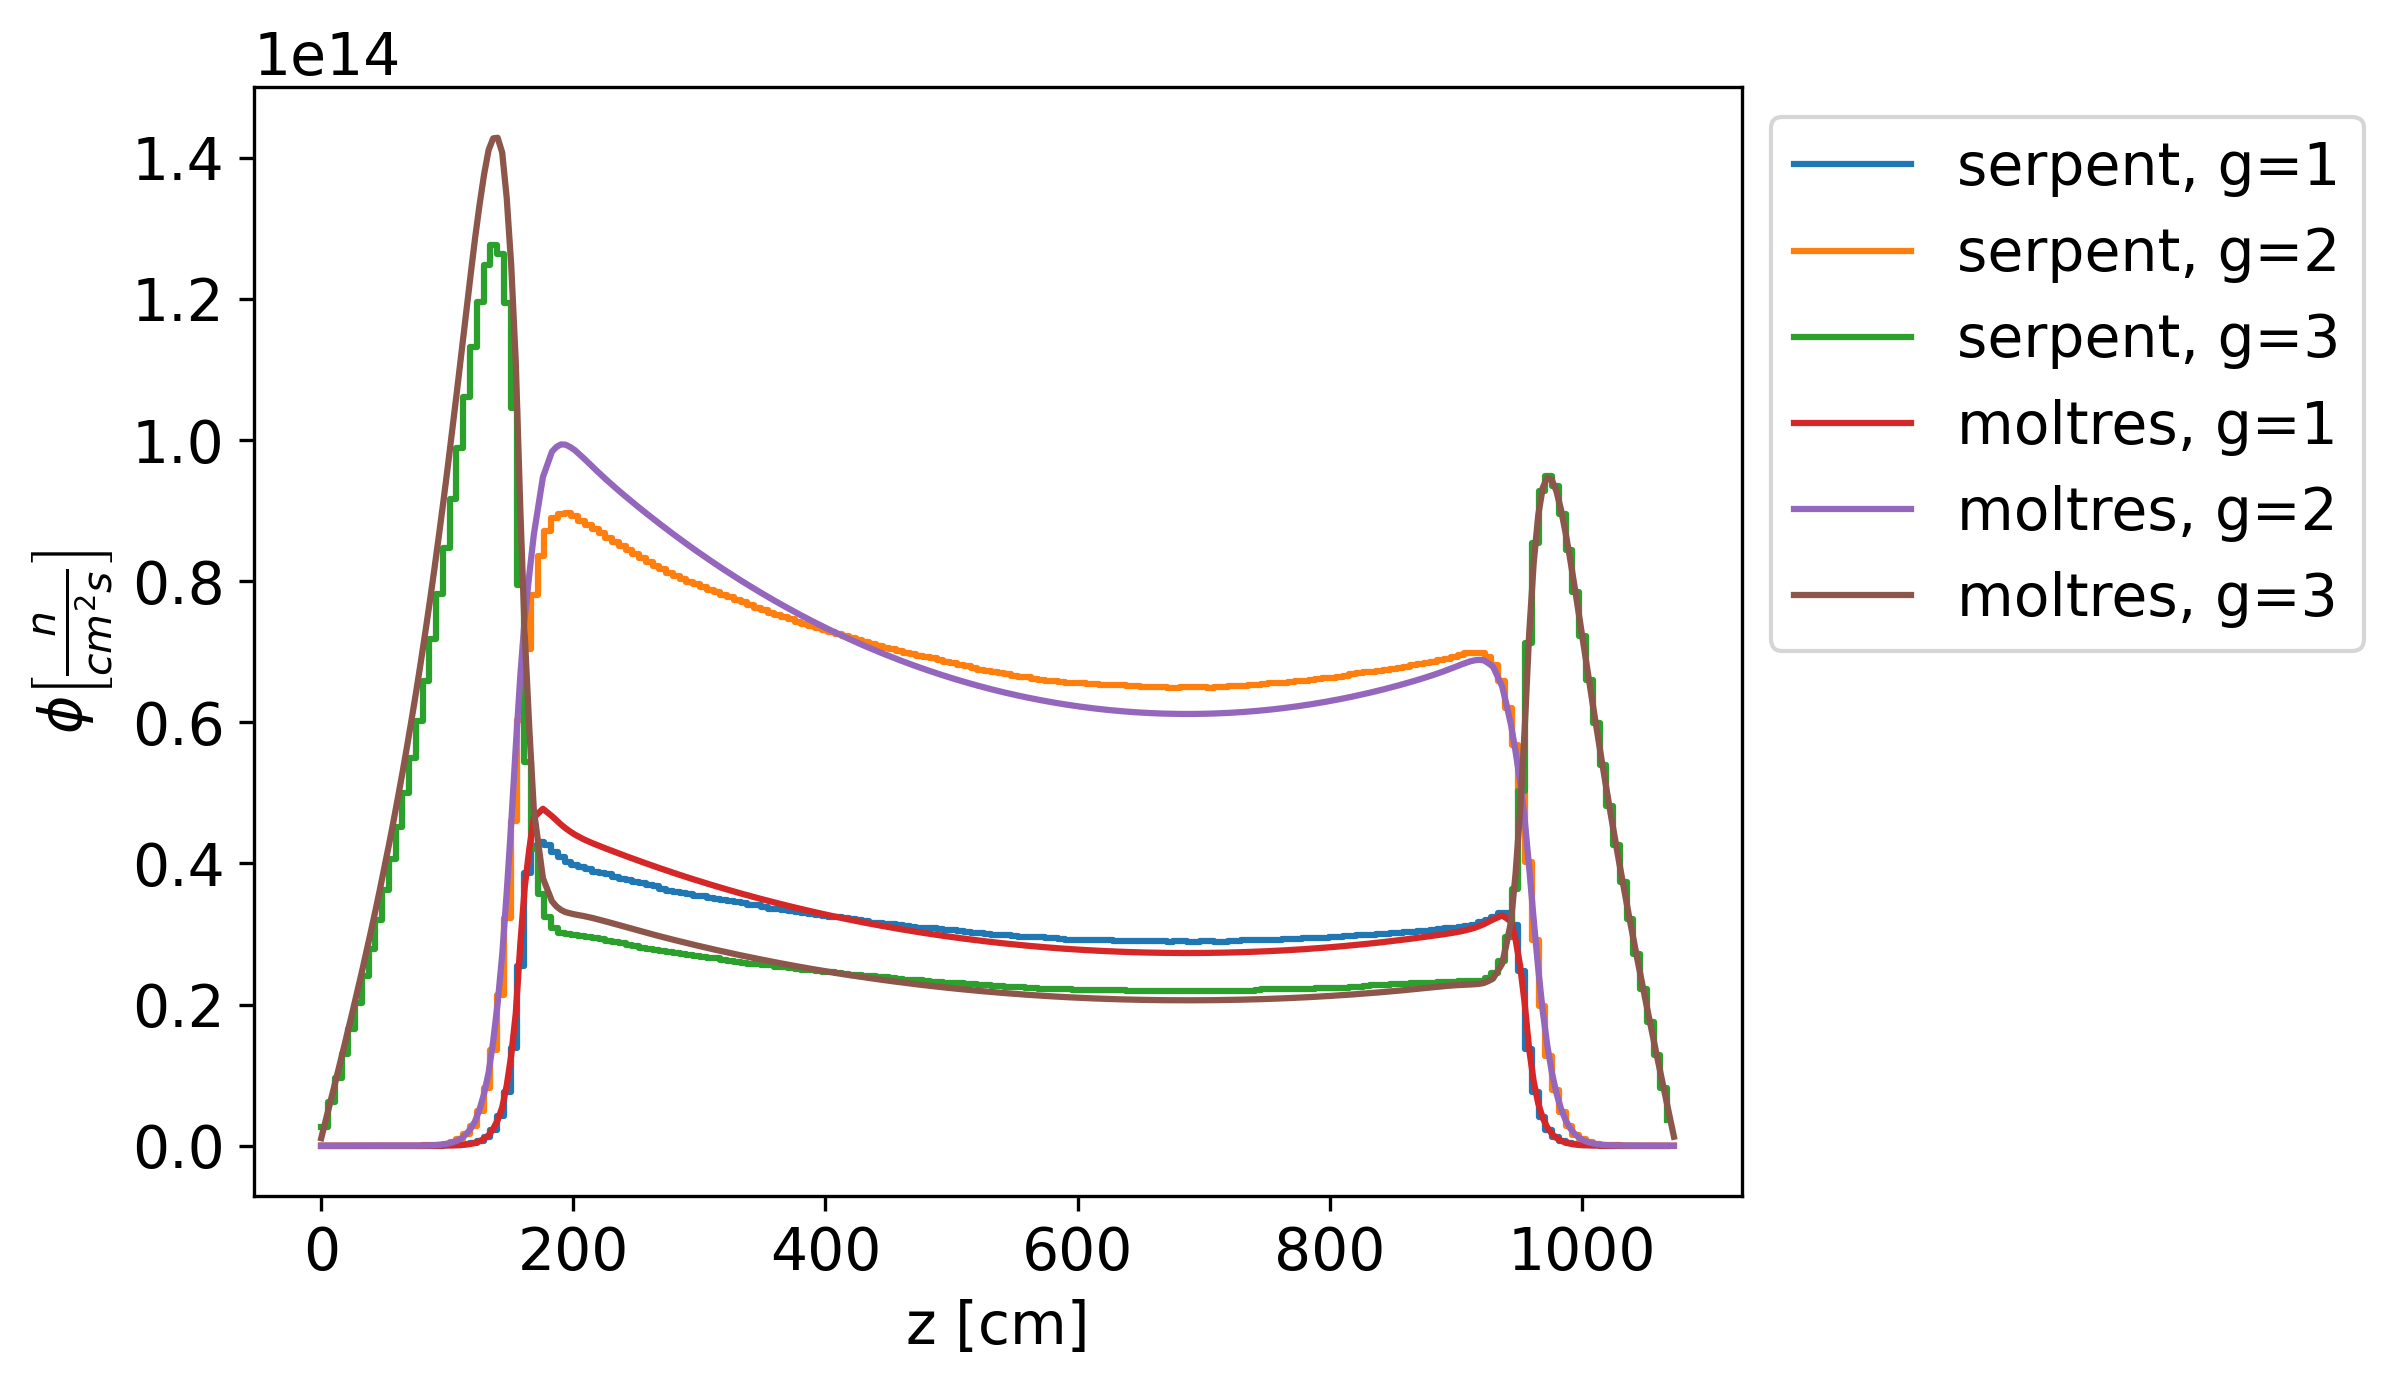
\includegraphics[width=0.51\textwidth]{figures-neutronics/serpent-moltres-LBP-1200-fluxes}
    }
    \subfloat[Relative difference between Serpent and Moltres neutron fluxes.]{
        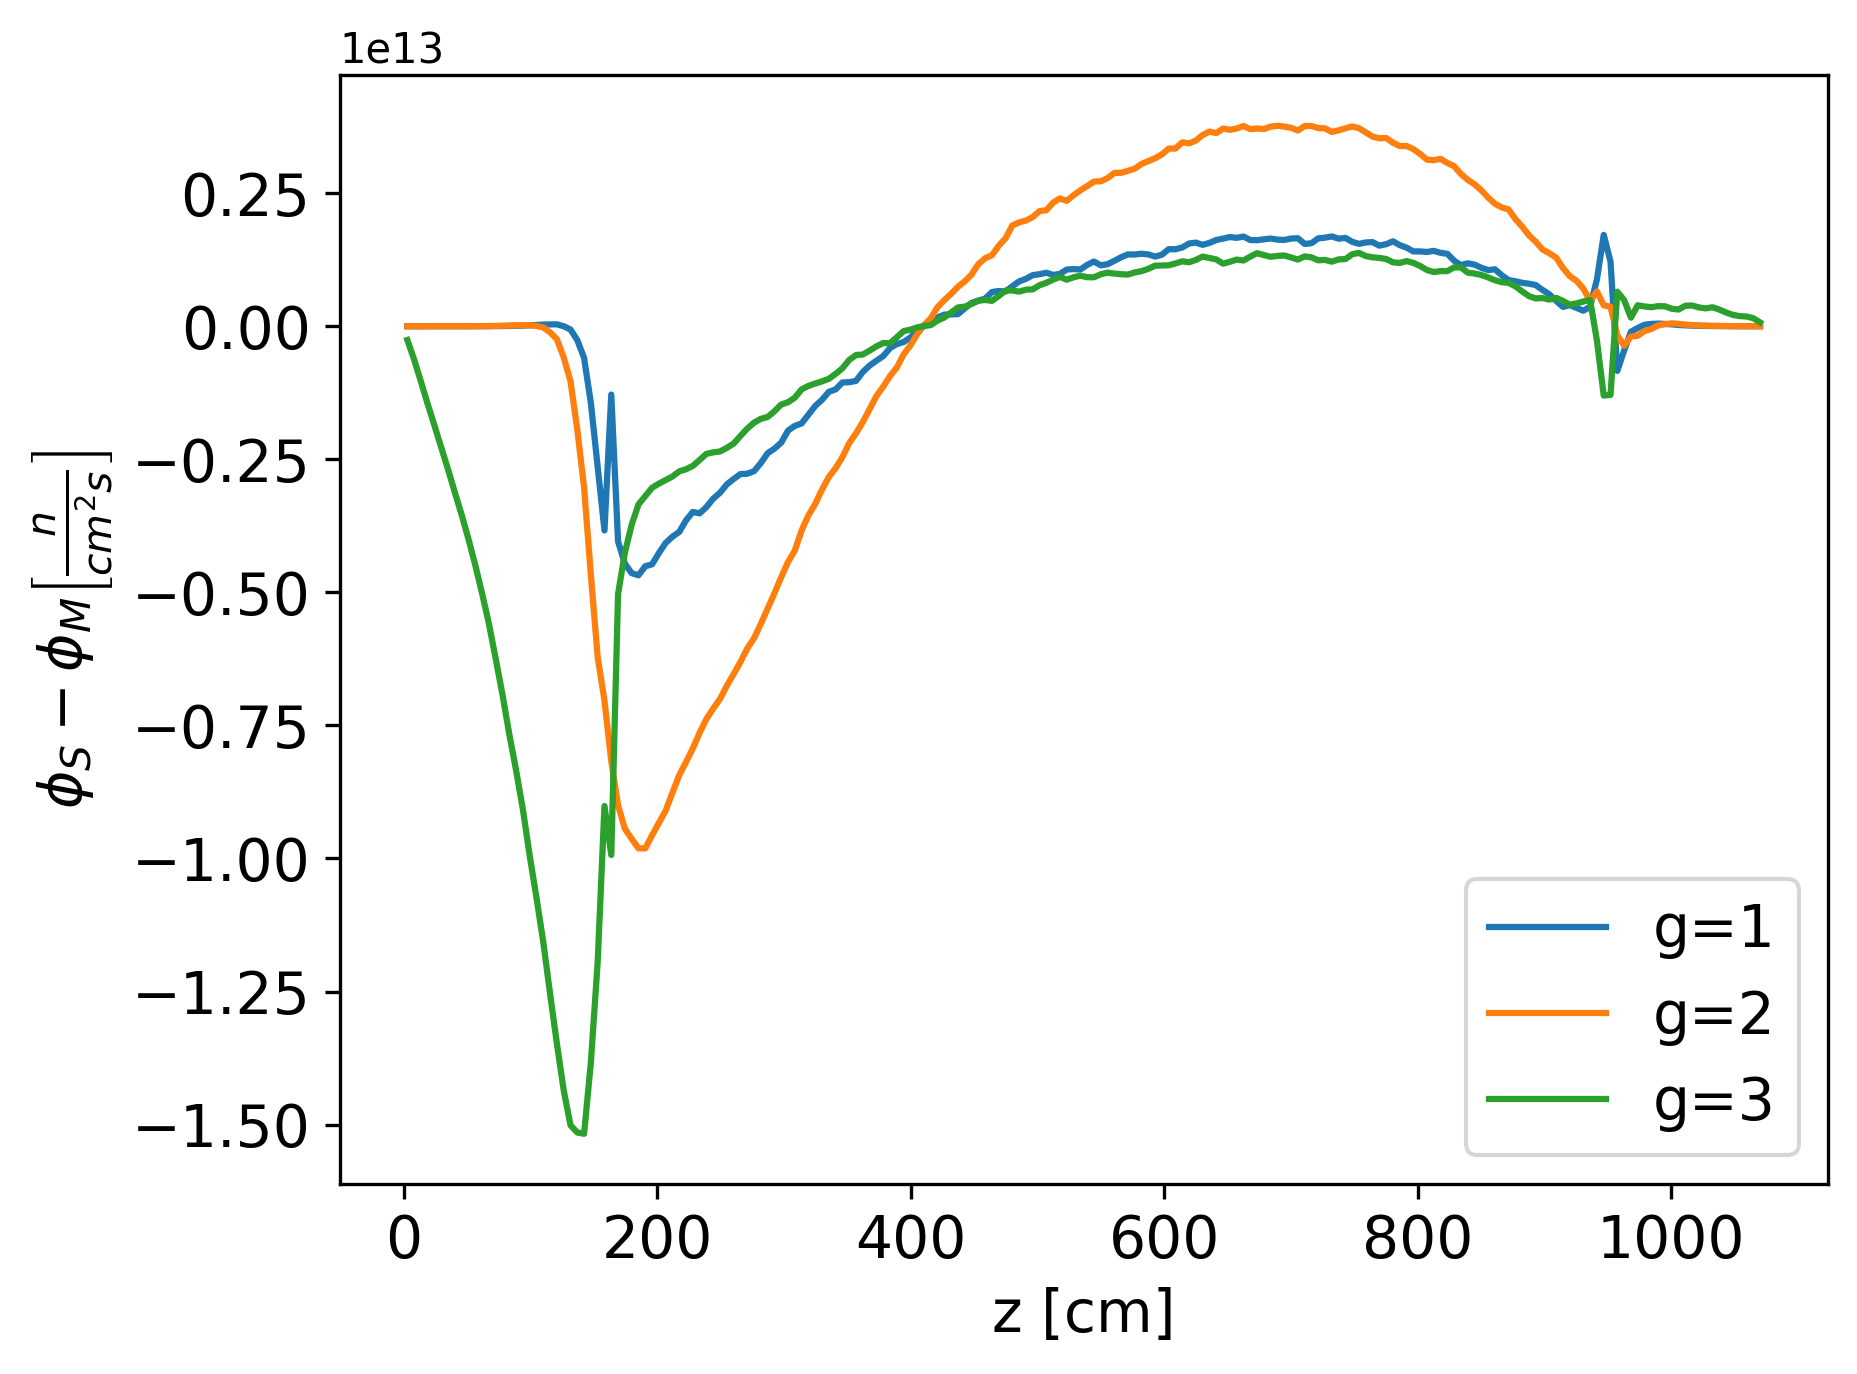
\includegraphics[width=0.39\textwidth]{figures-neutronics/serpent-moltres-LBP-1200-error}
    }
  \hfill
  \caption{Operational case 4: fuel column with burnable poisons at 1200K. Comparison of Serpent and Moltres-derived 3-group axial neutron fluxes.}
  \label{fig:assembly-LBP-1200-flux}
\end{figure}

Table \ref{tab:keff} exhibits the eigenvalues calculated by Serpent and $\Delta \rho$, calculated with equation \ref{eq:delta-rho}, for the different energy group structures.
The eigenvalues in Moltres differ slightly from the eigenvalues in Serpent, and overall, the reactivity difference is less than 50 pcm.
The number of energy groups does not affect the accuracy of the eigenvalue calculations in Moltres.

\begin{table}[htbp!]
  \centering
  \caption{Eigenvalues calculated by Serpent and reactivity difference between eigenvalues calculated by Moltres and Serpent, see equation \ref{eq:delta-rho}, for the different energy group structures.}
  \begin{tabular}{c|c|cccccccc}
  \toprule
Operational case  & Serpent       & \multicolumn{8}{c}{$\Delta \rho$ [pcm]/Energy groups}            \\ \cline{3-10} 
                  & eigenvalues   & 3   & 6   & 9   & 12   & 15   & 18   & 21   & 26   \\
  \midrule
1 & 1.43800 $\pm$ 0.00008 & 10  & 7   & 6   & 6    & 5    & 6    & 6    & 12   \\
2 & 1.37771 $\pm$ 0.00008 & 23  & 15  & 4   & 3    & 2    & 2    & 1    & 11   \\
3 & 1.12861 $\pm$ 0.00009 & 44  & 21  & 24  & 25   & 25   & 24   & 19   & 9    \\
4 & 1.06554 $\pm$ 0.00010 & 36  & 40  & 29  & 32   & 44   & 43   & 25   & 25   \\
  \bottomrule
  \end{tabular}
  \label{tab:keff}
\end{table}

The last analysis is for the Moltres axial flux.
Considering the 26 group structure as the reference value, equation \ref{eq:l2norm} obtained the $L_2$-norm of the active core's axial flux relative difference
\begin{align}
  & \Delta_{L_2} = \left\| \frac{\phi_G(z)-\phi_{ref}(z)}{\phi_{ref}(z)} \right\|  \quad \wedge \quad z\quad \in \quad L_a \label{eq:l2norm}
  \intertext{where}
  & \Delta_{L_2} = \mbox{L$_2$-norm relative difference } [-] \notag \\
  & \phi_G(z) = \mbox{$G$-energy groups axial flux } [n \cdot cm^{-2} \cdot s^{-1}] \notag \\
  & \phi_{ref}(z) = \mbox{reference axial flux } [n \cdot cm^{-2} \cdot s^{-1}] \notag \\
  & L_a = \mbox{active core length } [cm]. \notag
\end{align}

Figures \ref{fig:assembly-noLBP-er} and \ref{fig:assembly-LBP-er} show $\Delta_{L_2}$ for the various energy group structures.
Overall, the relative error decreases with an increase in the number of energy groups.
Nonetheless, this is not always the case.
For example, in Figure \ref{fig:assembly-noLBP-er-b}, the thermal flux agreement improves from 12 to 15-energy groups, but the fast flux agreement worsens.
Additionally, the relative error of the cases with no burnable poisons is smaller than the relative error of the cases with burnable poison.
The treatment of the burnable poisons challenges the accuracy of the homogenized simulations in Moltres.
Three, six, and nine energy-groups yield more than 50$\%$ error when treating the burnable poison, Figure \ref{fig:assembly-LBP-er}.

% No LBP
\begin{figure}[htbp!]
	\centering
    \subfloat[Operational case 1: 600K.]{
        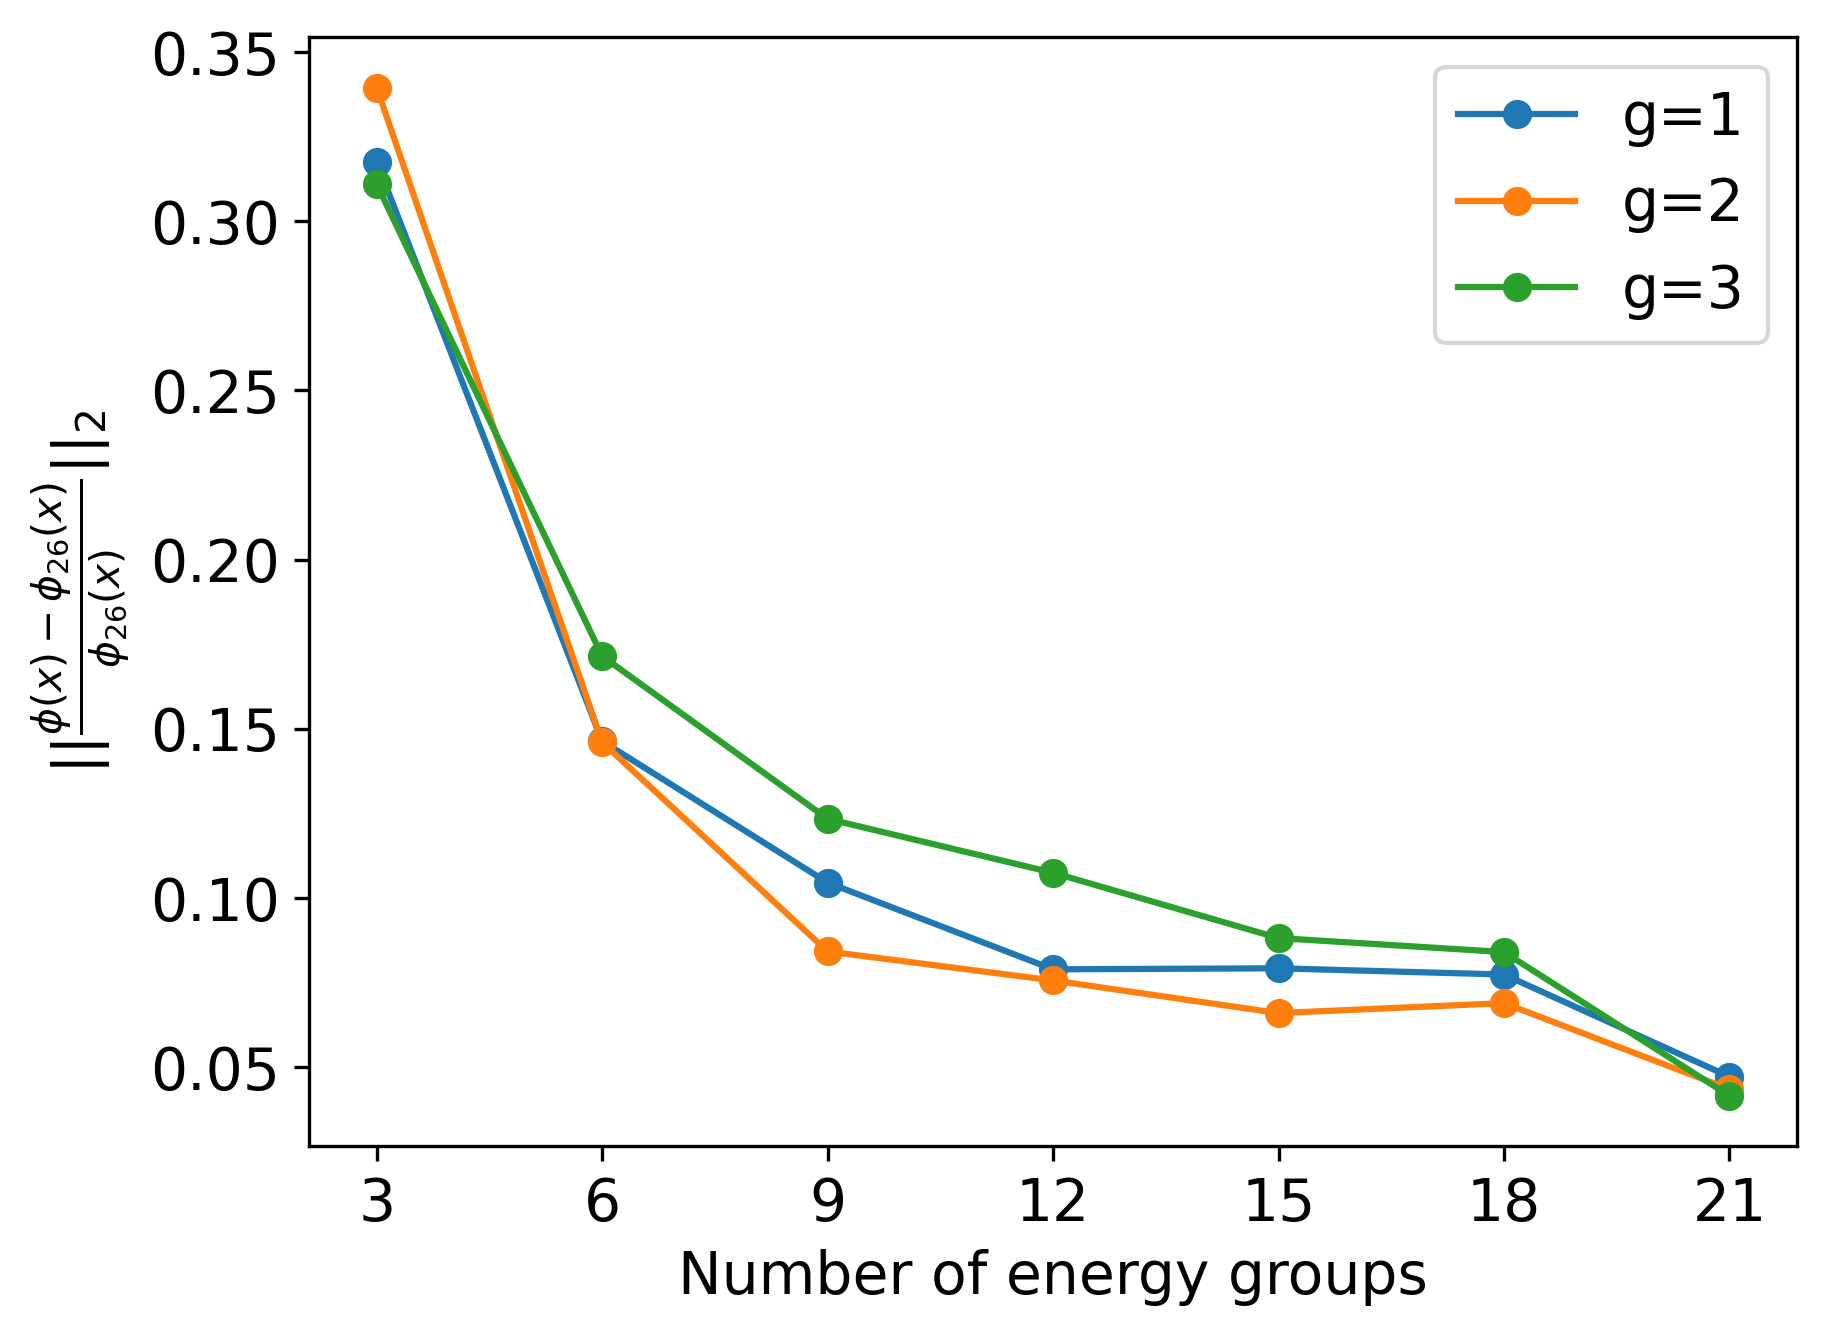
\includegraphics[width=0.45\textwidth]{figures-neutronics/noLBP-600-er-final}
    }
    \subfloat[Operational case 2: 1200K.\label{fig:assembly-noLBP-er-b}]{
        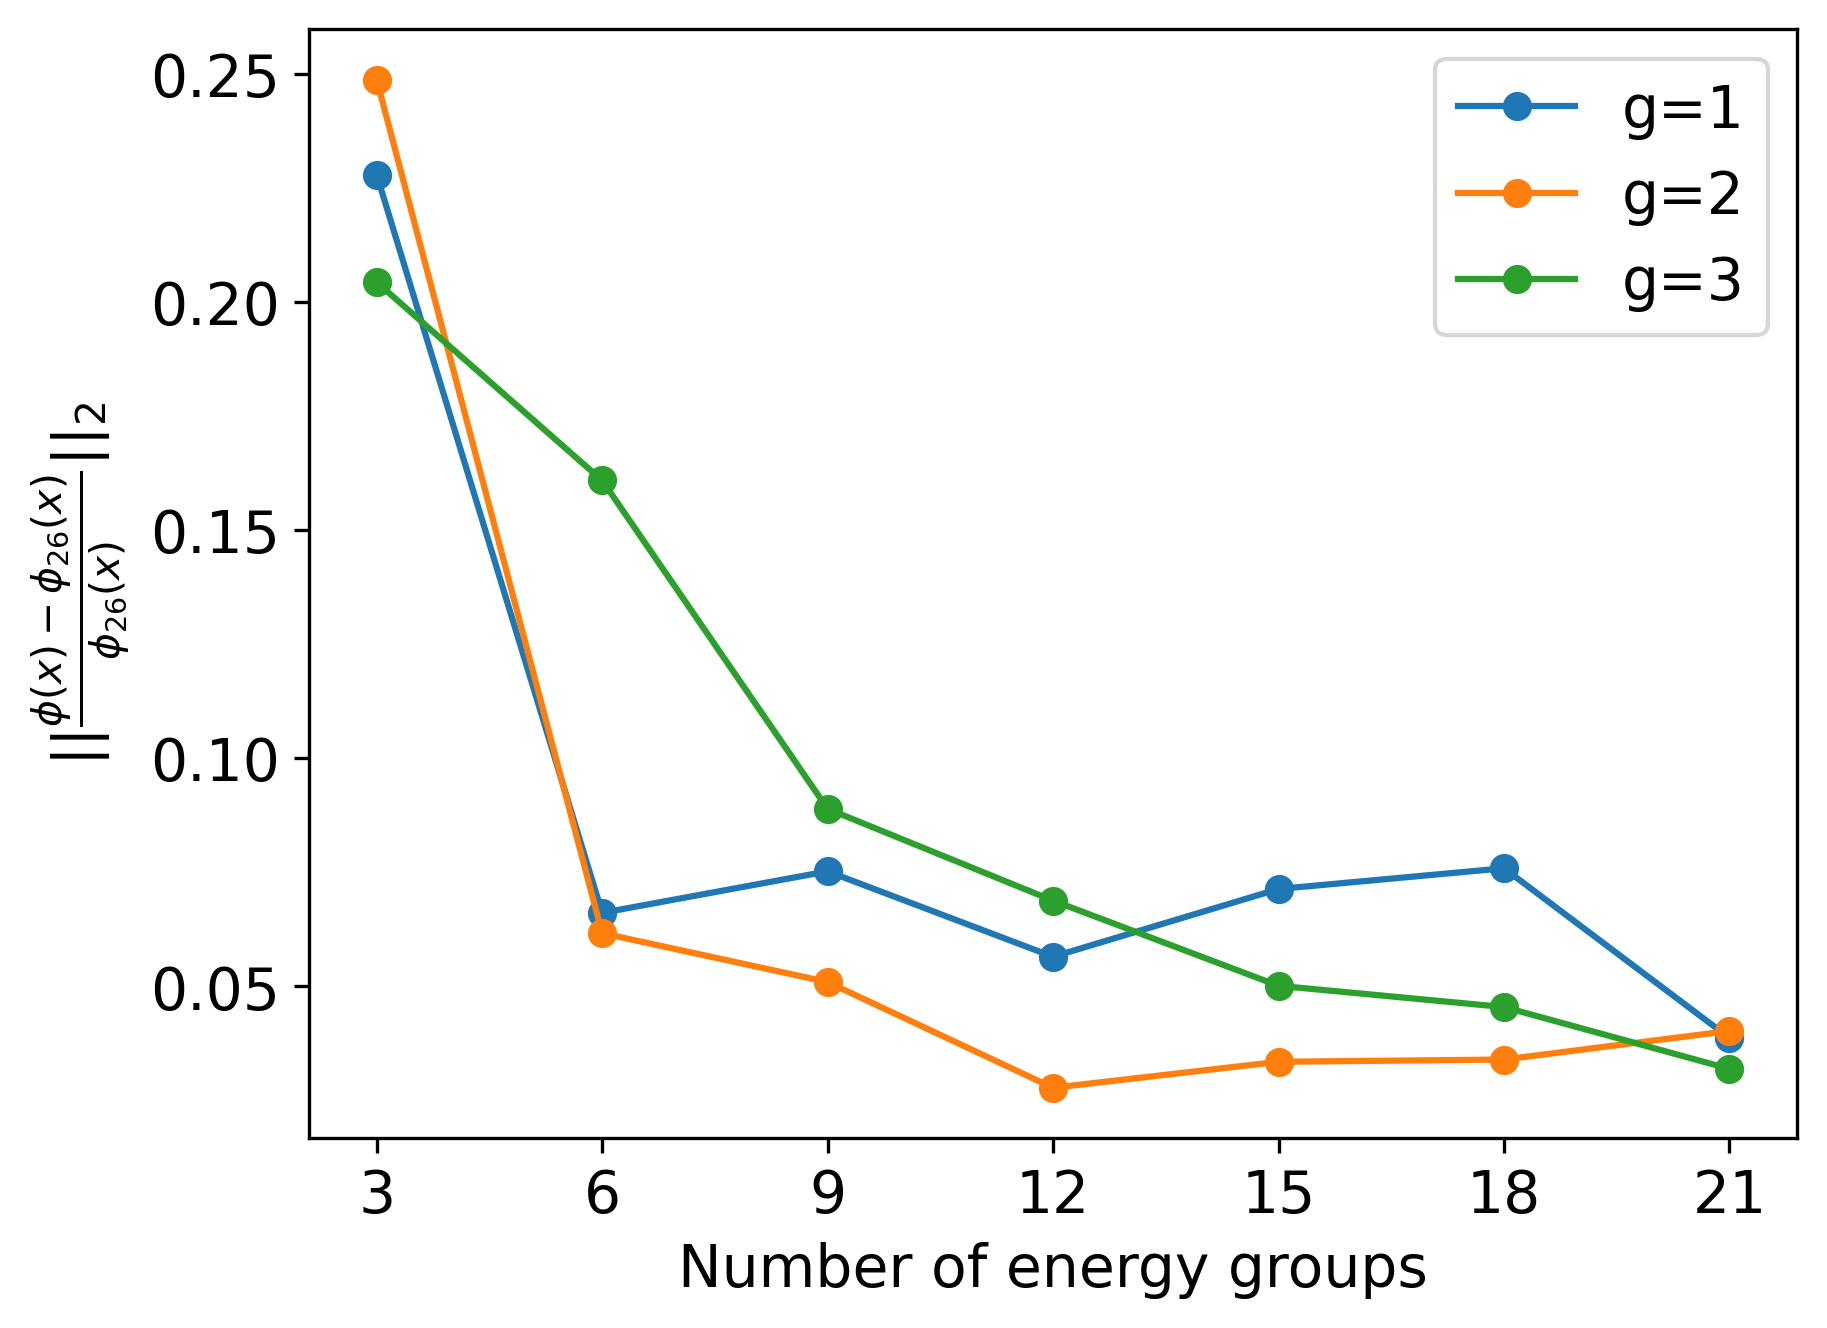
\includegraphics[width=0.45\textwidth]{figures-neutronics/noLBP-1200-er-final}
    }
	\hfill
    \caption{L$_2$-norm relative error for different number of energy group structures for the operational cases with no burnable poisons.}
	\label{fig:assembly-noLBP-er}
\end{figure}

% LBP
\begin{figure}[htbp!]
	\centering
    \subfloat[Operational case 3: 600K.]{
        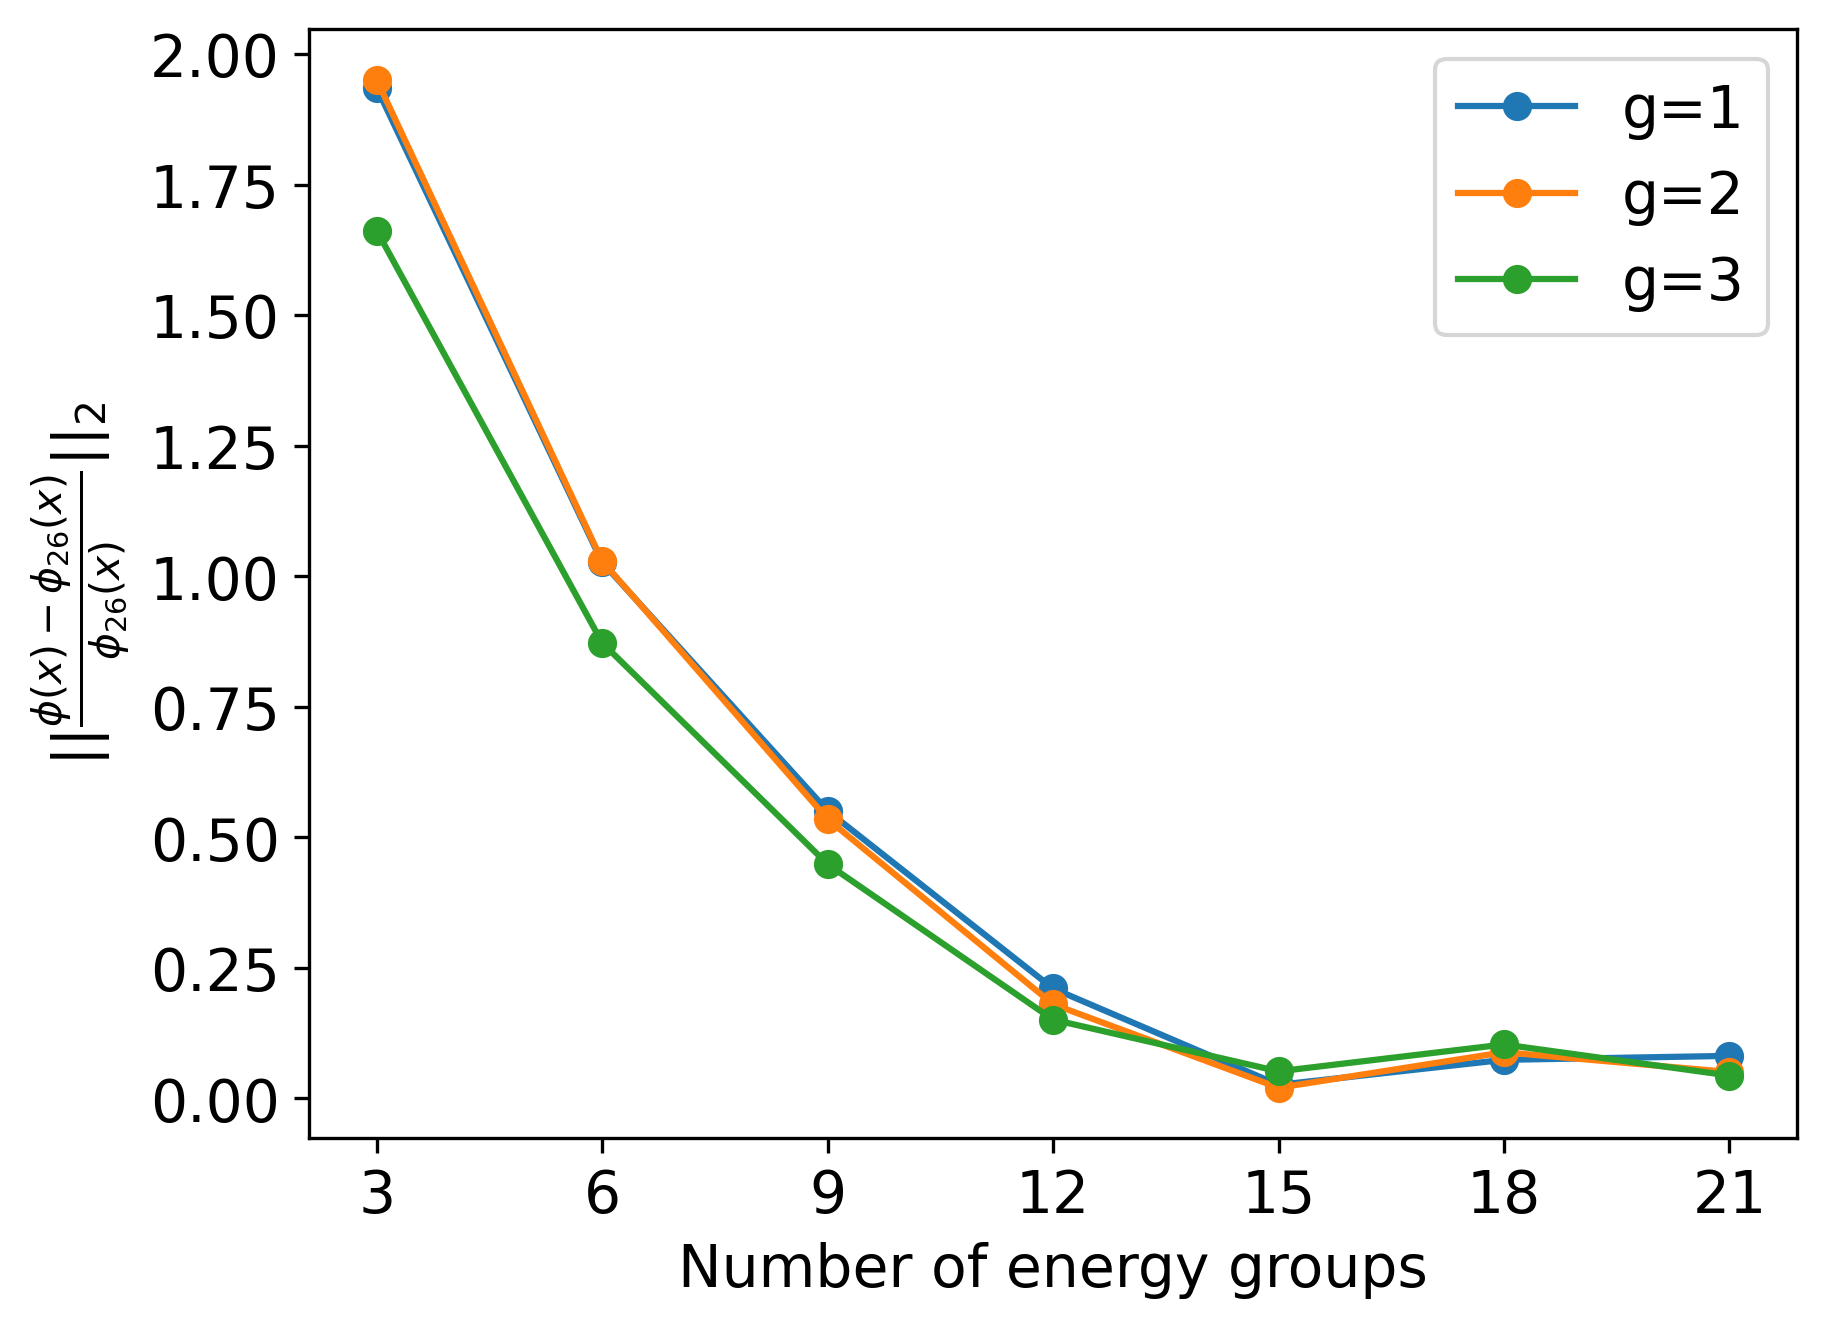
\includegraphics[width=0.45\textwidth]{figures-neutronics/LBP-600-er-final}
    }
    \subfloat[Operational case 4: 1200K.]{
        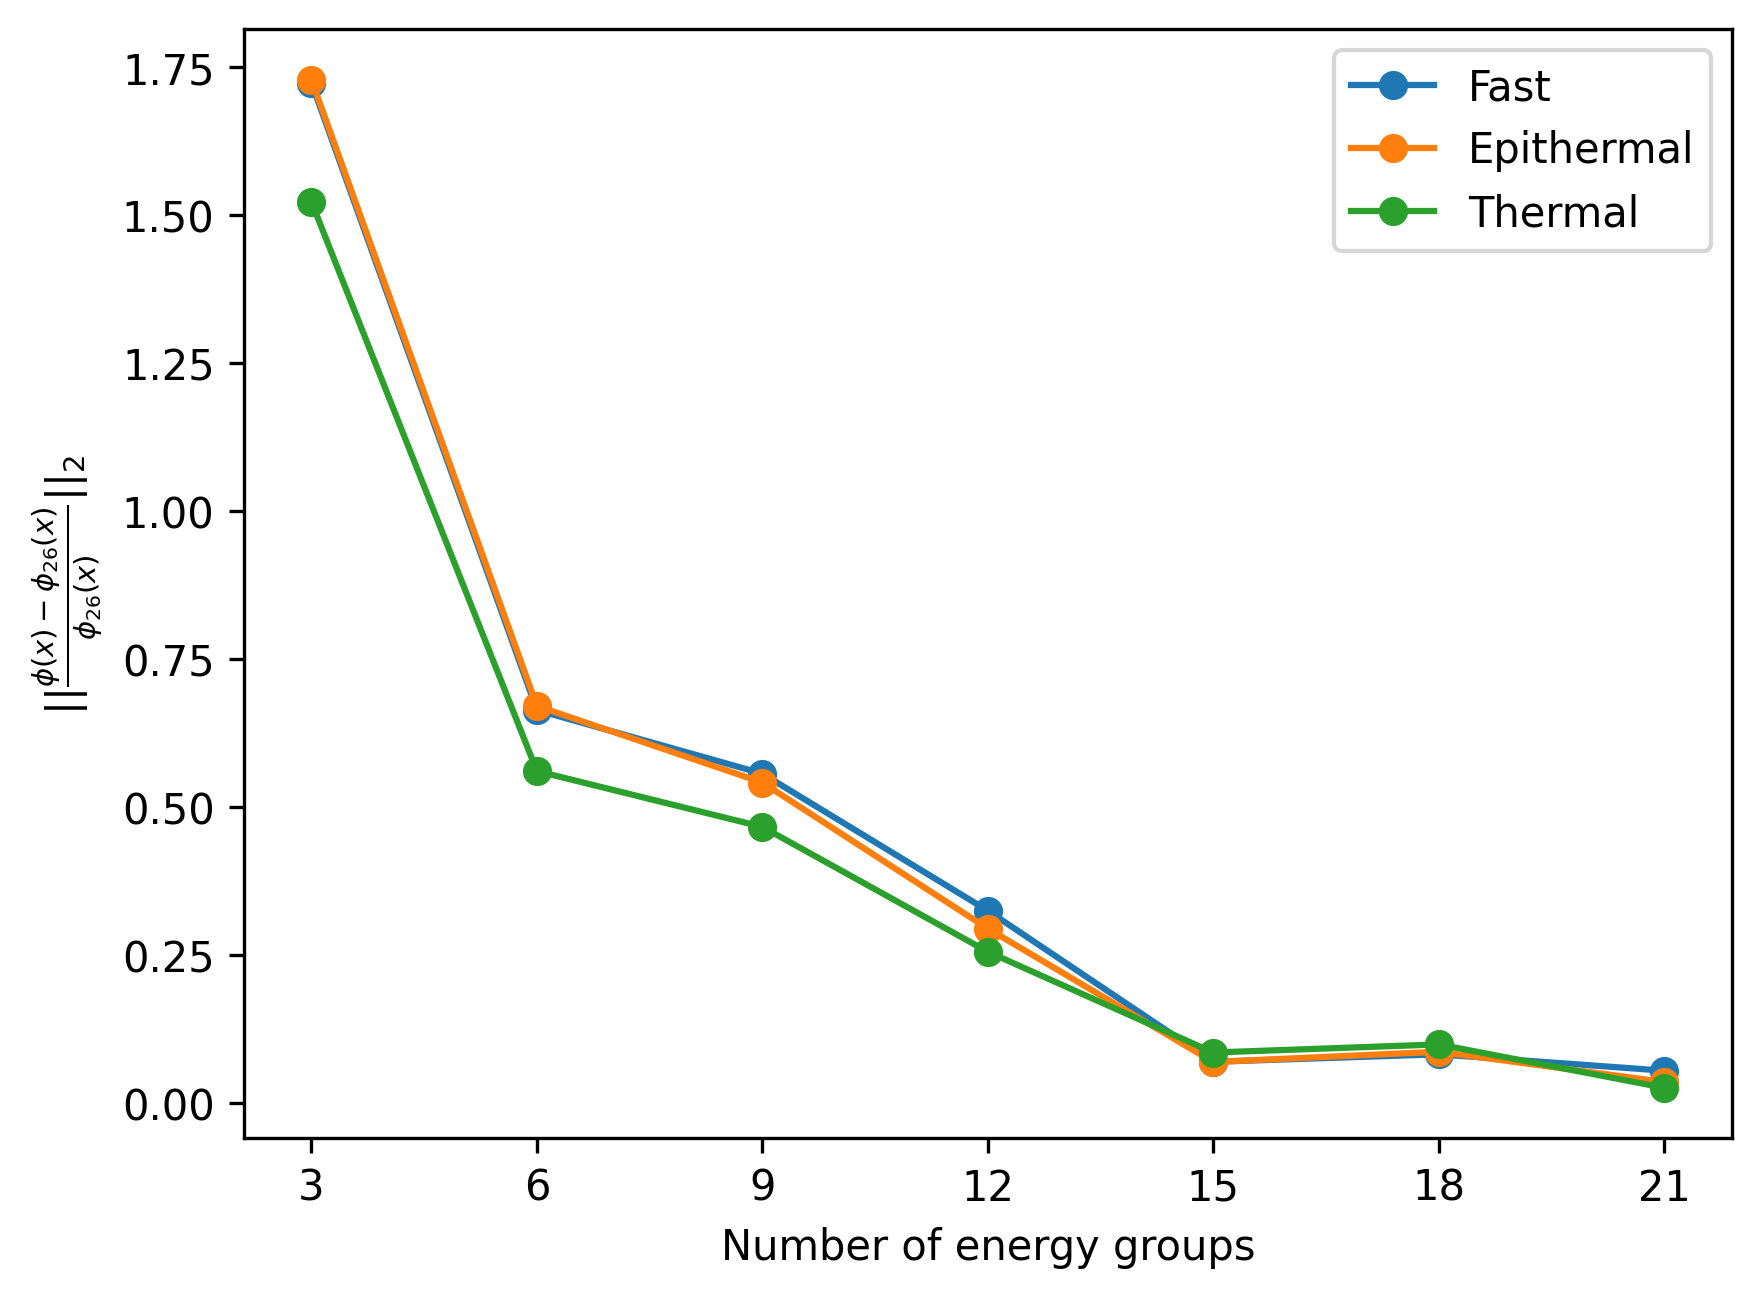
\includegraphics[width=0.45\textwidth]{figures-neutronics/LBP-1200-er-final}
    }
	\hfill
    \caption{LBP case. L$_2$-norm relative error for different number of energy group structures for the operational cases with burnable poisons.}
	\label{fig:assembly-LBP-er}
\end{figure}

The analysis also included the computational time and the peak memory usage during the simulations, as shown in Figure \ref{fig:assembly-time}.
All the simulations used 128 cores.
This section presents only the cases at 600K because the impact of the temperature change was not significant.
The computational requirements rise with an increase in the number of energy groups.
As the geometry uses a constant number of elements, the number of DoFs per energy-group remains constant for all the simulations.
Figure \ref{fig:assembly-time} also shows that the overall time of the cases with burnable poison is higher than the cases without them.

% Time and memory
\begin{figure}[htbp!]
	\centering
    \subfloat[No burnable poisons at 600 K.]{
        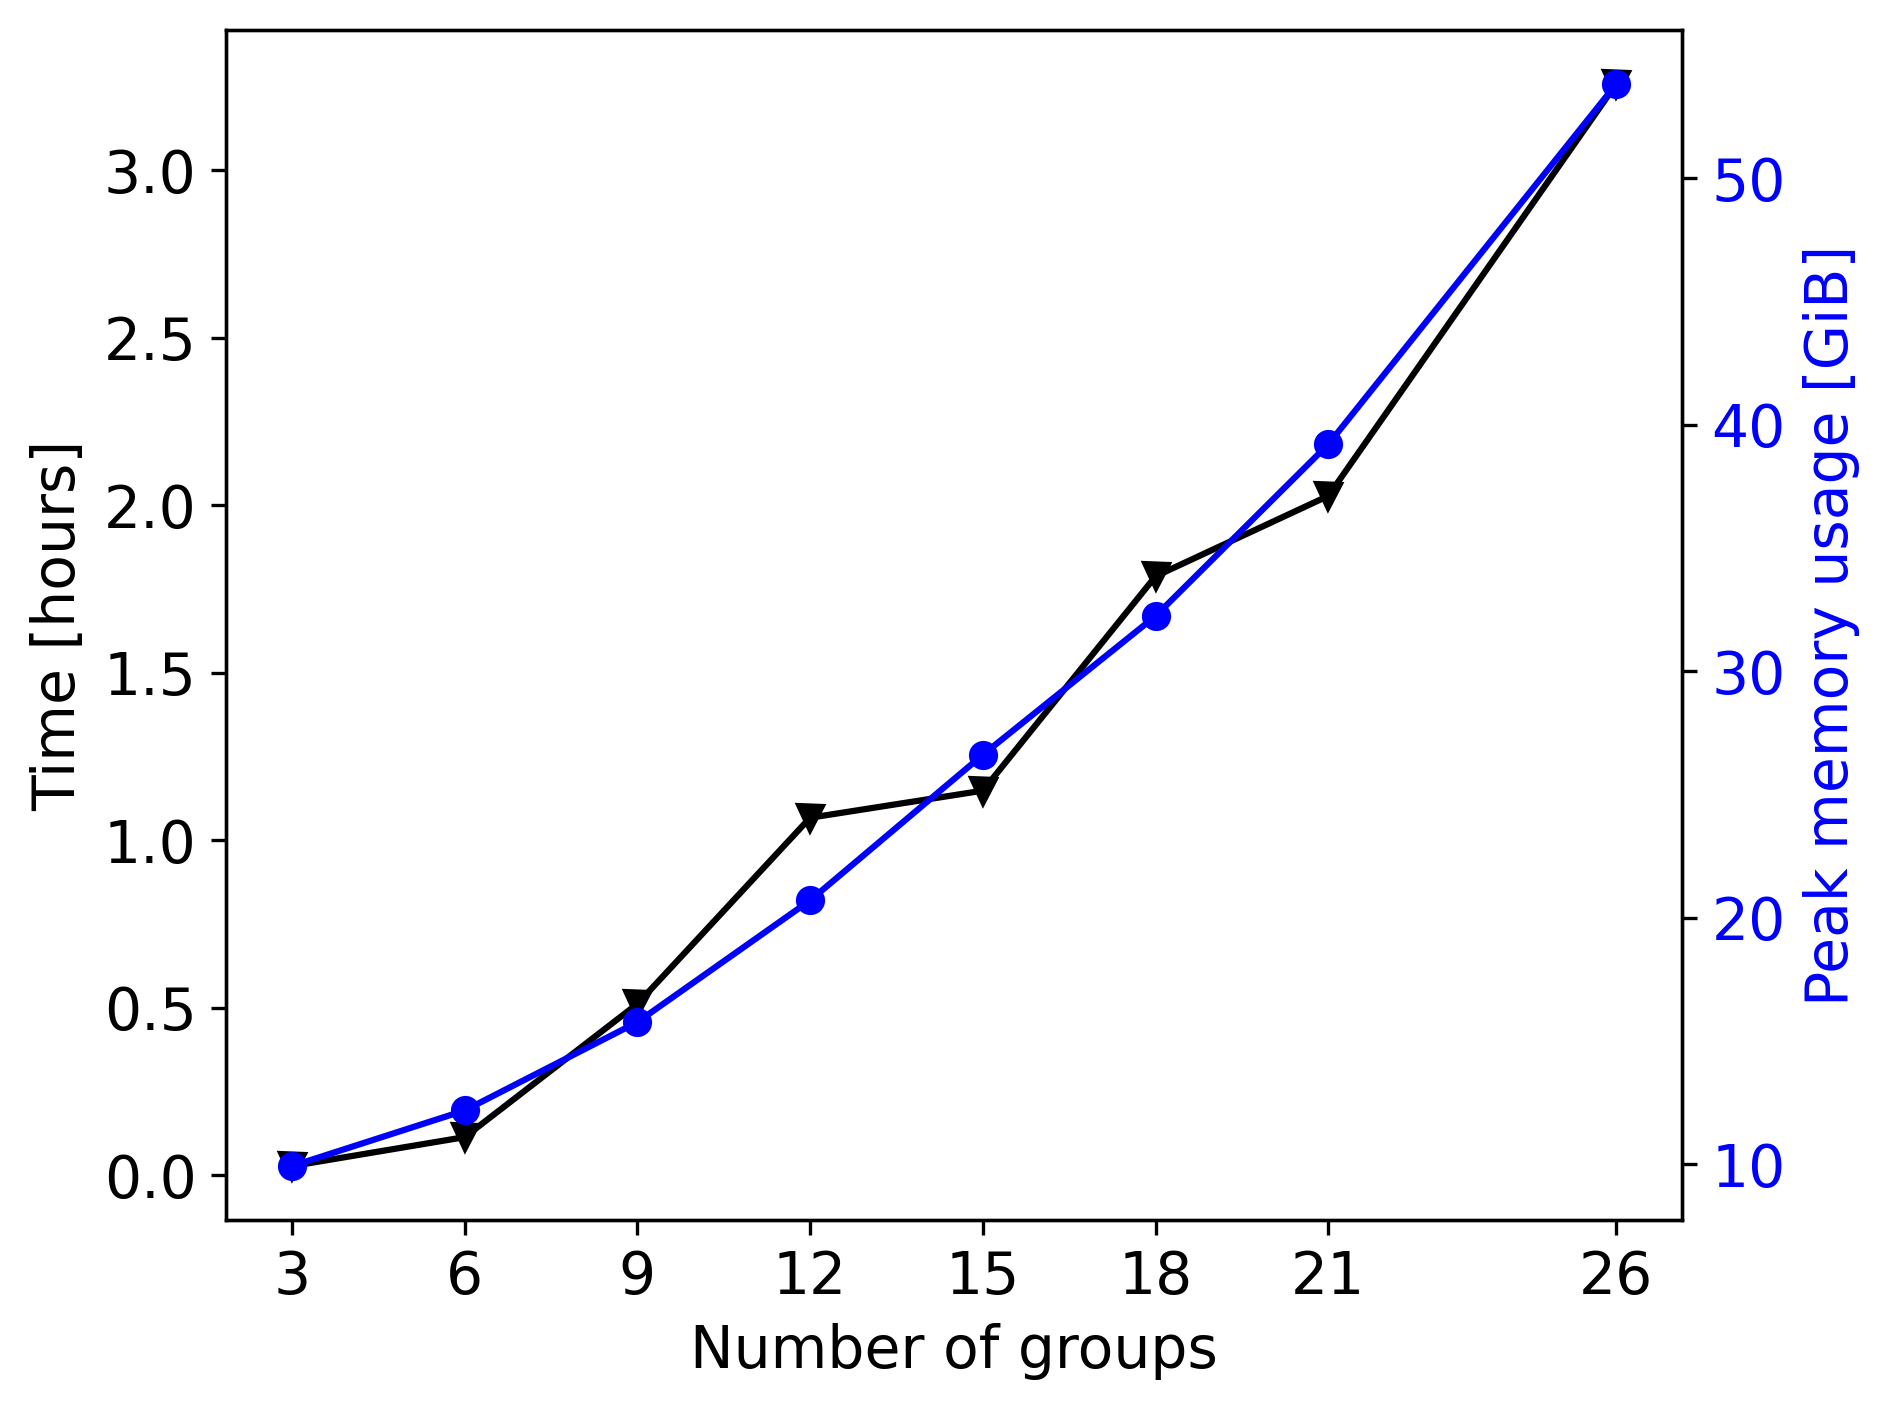
\includegraphics[width=0.45\textwidth]{figures-neutronics/time-noLBP-600}
    }
    \subfloat[Burnable poisons at 600 K.]{
        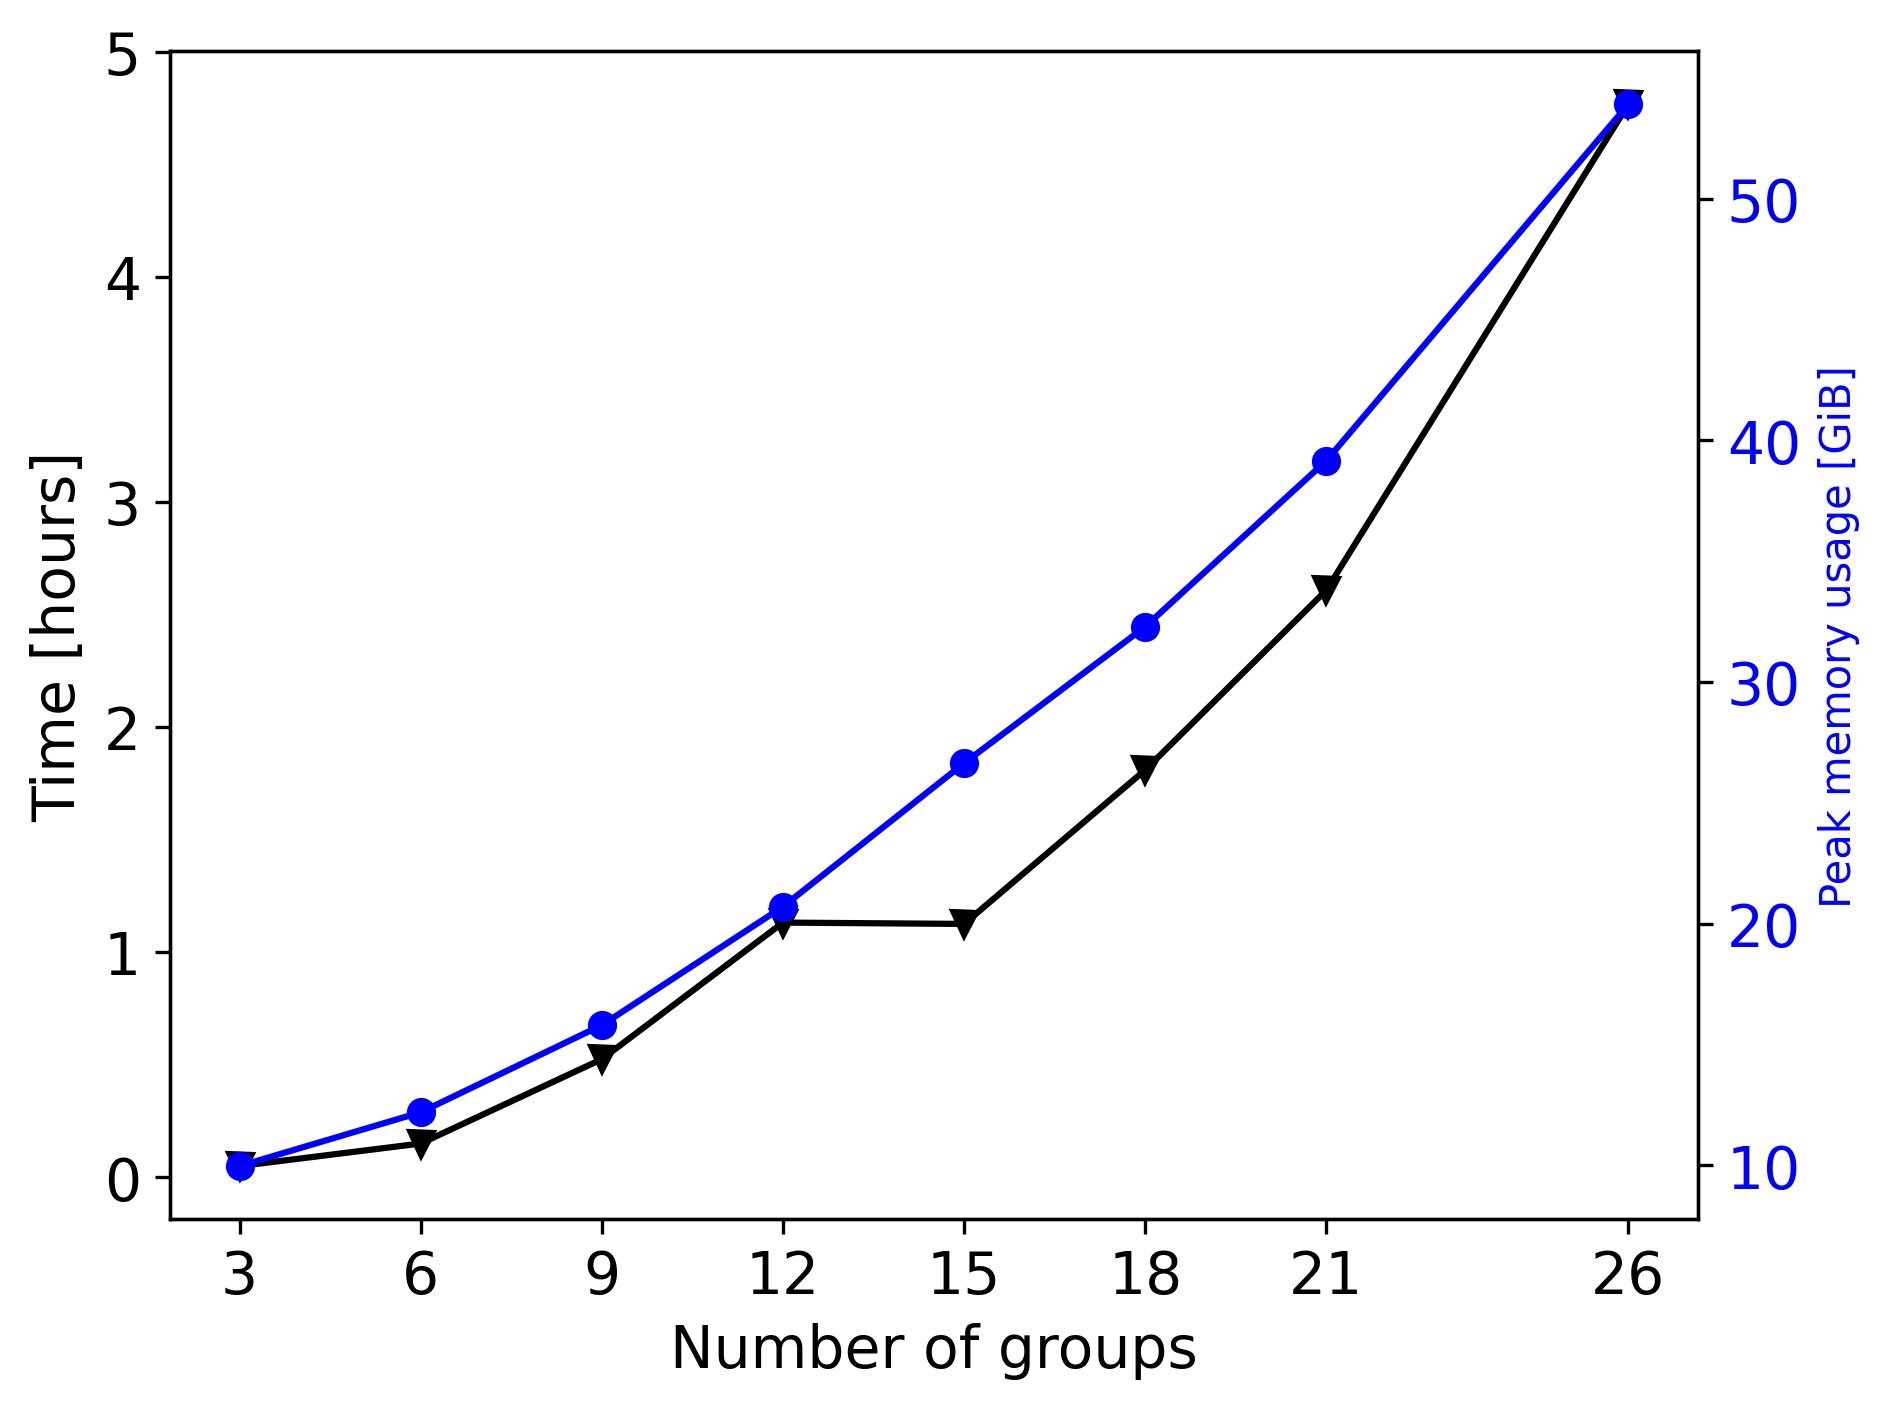
\includegraphics[width=0.45\textwidth]{figures-neutronics/time-LBP-600}
    }
	\hfill
	\caption{Computational time and memory requirements for different number of energy group structures.}
	\label{fig:assembly-time}
\end{figure}

The last study analyzed the impact of the energy group structure on the flux accuracy for a constant number of energy groups.
Fifteen energy groups are the preferred choice, as it yields a good overall accuracy and a practical computational expense.
Table \ref{tab:energygroups} defines various energy group structures.
Table \ref{tab:accuracy15} displays the $L_2$-norm of the relative error for the various energy group structures.
Some energy group structures yield better results for some cases while giving worse results for others.
For example, the $15d$ structure gives better results at 600K with burnable poisons than without them.
To choose the best performing structure, equation \ref{eq:weighted-ave} calculated a weighted average for the different groups
\begin{align}
  & W_{ave} = w_{th} \Delta_{th} + w_{epi} \Delta_{epi} + w_{f} \Delta_{f} \label{eq:weighted-ave}
  \intertext{where}
  & W_{ave} = \mbox{weighted average } [-] \notag \\
  & w_{th} = \mbox{thermal flux weight } [-] \notag \\
  & w_{epi} = \mbox{epipthermal flux weight } [-] \notag \\
  & w_{f} = \mbox{fast flux weight } [-] \notag \\
  & \Delta_{th} = \mbox{L$_2$-norm relative difference of the thermal flux } [-] \notag \\
  & \Delta_{epi} = \mbox{L$_2$-norm relative difference of the epithermal flux } [-] \notag \\
  & \Delta_{f} = \mbox{L$_2$-norm relative difference of the fast flux } [-]. \notag
\end{align}

The arbitrary choice of the weights of 0.5, 0.3, and 0.2 for the thermal, epithermal, and fast fluxes for a weighted average yields the energy group structure $15d$ as the best one.

\begin{table}[htbp!]
  \centering
  \caption{Axial flux relative difference $L_2$-norm for various energy group structures. Values expressed in [\%].}
  \begin{tabular}{@{}c| c l S[table-format=2.1] S[table-format=2.1] S[table-format=2.1] S[table-format=2.1] S[table-format=2.1] }
  \toprule
	Burnable poisons     & Temperature {[}K{]}   & Flux       & \multicolumn{1}{c@{}}{15a} & \multicolumn{1}{c@{}}{15b}  & \multicolumn{1}{c@{}}{15c}  & \multicolumn{1}{c@{}}{15d}  & \multicolumn{1}{c@{}}{15e}  \\
	\midrule
	\multirow{6}{*}{No}  & \multirow{3}{*}{600}  & Fast       & 7.9  & 8.0  & 8.2  & 8.1  & 9.1  \\
	                     &                       & Epithermal & 6.6  & 6.5  & 8.6  & 8.2  & 9.2  \\
	                     &                       & Thermal    & 8.8  & 8.5  & 10.6 & 10.7 & 12.9 \\ \cline{2-8}
	                     & \multirow{3}{*}{1200} & Fast       & 7.1  & 7.7  & 5.7  & 5.1  & 4.5  \\
	                     &                       & Epithermal & 3.3  & 3.9  & 6.2  & 5.1  & 3.4  \\
	                     &                       & Thermal    & 5.0  & 4.7  & 8.5  & 8.2  & 8.4  \\ \hline
	\multirow{6}{*}{Yes} & \multirow{3}{*}{600}  & Fast       & 24.0 & 24.8 & 2.6  & 2.3  & 3.7  \\
	                     &                       & Epithermal & 21.0 & 21.7 & 2.0  & 1.6  & 2.7  \\
	                     &                       & Thermal    & 18.1 & 18.8 & 5.2  & 5.5  & 5.7  \\ \cline{2-8}
	                     & \multirow{3}{*}{1200} & Fast       & 36.2 & 37.3 & 6.9  & 6.6  & 25.9 \\
	                     &                       & Epithermal & 33.2 & 34.2 & 6.9  & 6.5  & 25.1 \\
	                     &                       & Thermal    & 29.6 & 30.6 & 8.5  & 8.3  & 20.3 \\
	\midrule
	\multicolumn{2}{l}{Weighted average}         &            & 17.3 & 17.8 & 6.3  & 6.0  & 10.8 \\
	\bottomrule
  \end{tabular}
  \label{tab:accuracy15}
\end{table}


\subsection{Full-core}
\label{sec:neut-fullcore}

This section compares the results from Serpent and Moltres simulations of a full-core model.
Figure \ref{fig:fullcoremodel} displays a $xy$-plane of the model, which includes the bottom and top reflectors.
Due to symmetry, Moltres' model included only a $1/6^{th}$ of the reactor.
The first step in the calculation obtained the group constants using Serpent.
Tables \ref{tab:maincharac}, \ref{tab:element-characteristics}, and \ref{tab:compact} specify the model input parameters.
For simplicity, the model considered only standard fuel assemblies for all the fuel columns.
The model considered a fresh core, and it did not include the fuel handling holes nor the bottom and top reflector coolant channels.
Based on the previous section analyses, this analysis uses the energy group structure $15d$ from Table \ref{tab:energygroups}.
The material temperatures were 600K and 1200K, cases that represent the \gls{CZP} and the \gls{HFP} core states \cite{strydom_results_2015}.
The Serpent simulations included 8$\times 10^5$ neutrons per cycle, 500 active cycles, and 100 inactive cycles for the calculations.

% Geometries
\begin{figure}[htbp!]
	\centering
    \subfloat[Serpent model geometry.]{
        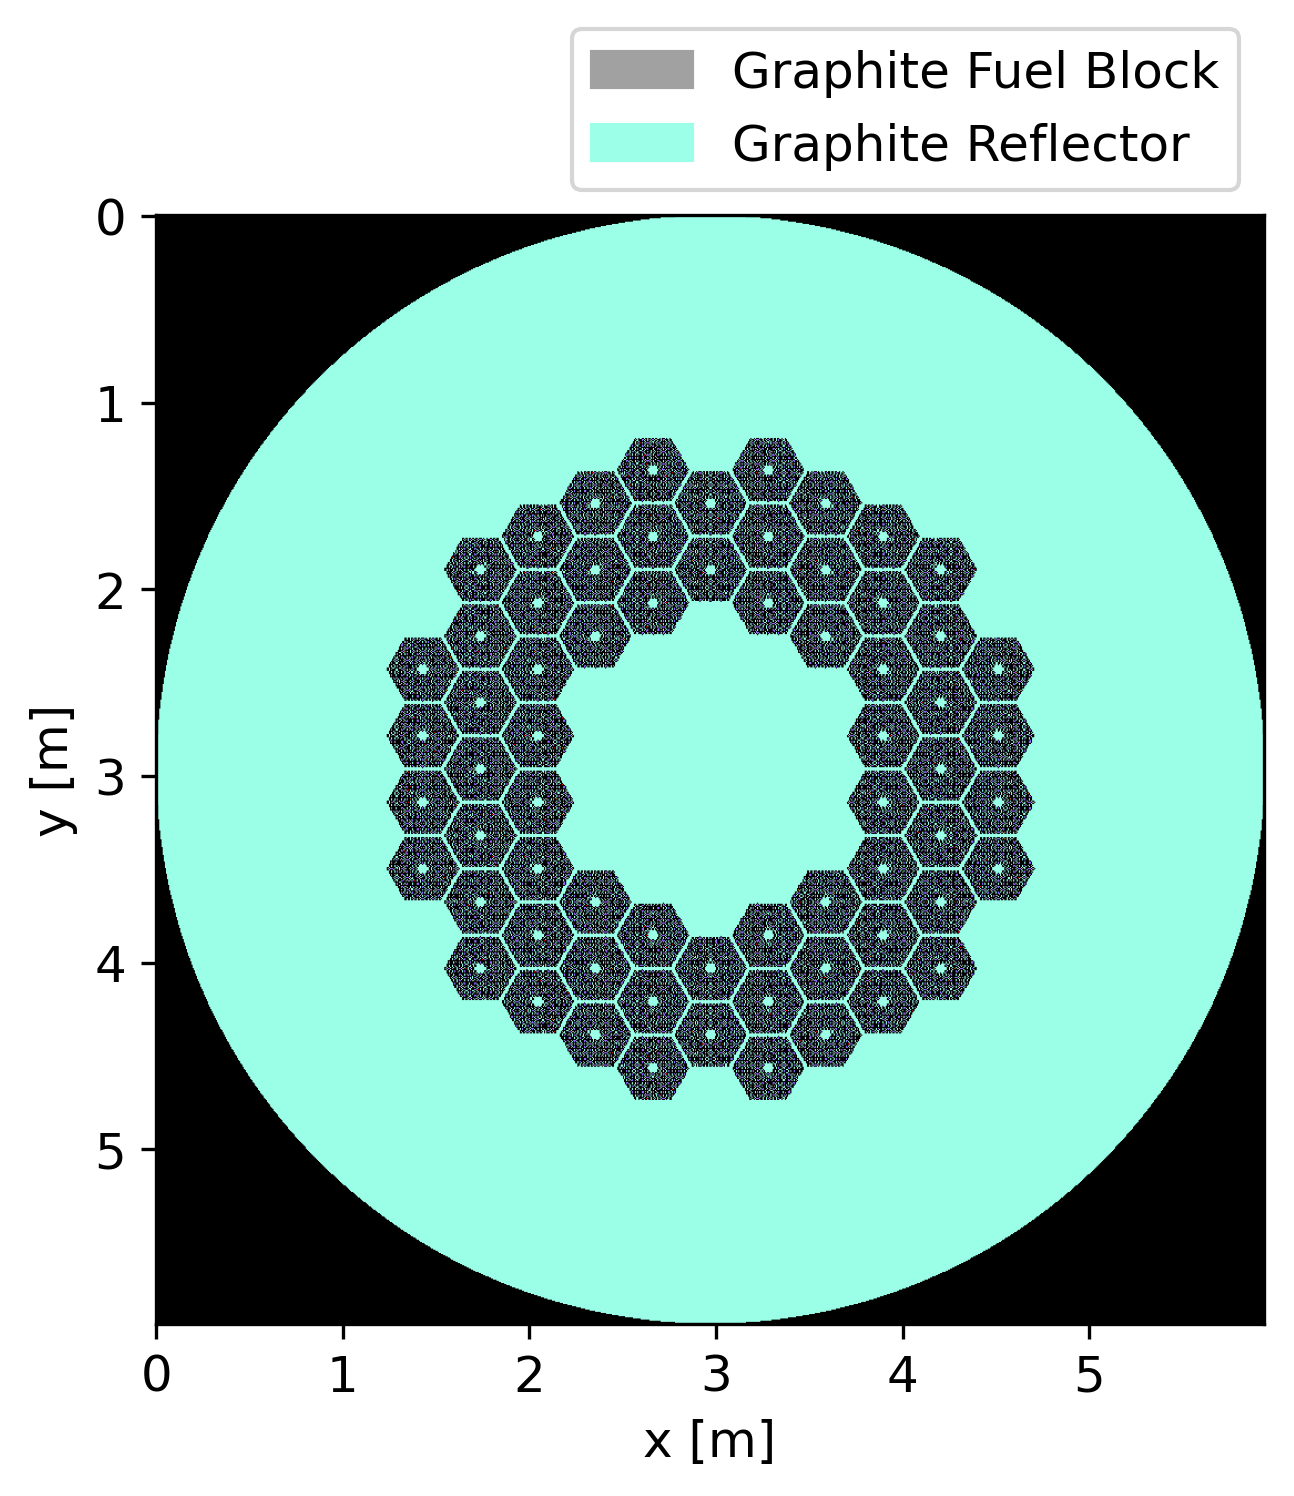
\includegraphics[width=0.48\textwidth]{figures-neutronics/oecd-fullcore}
    }
    \subfloat[Moltres model geometry.]{
        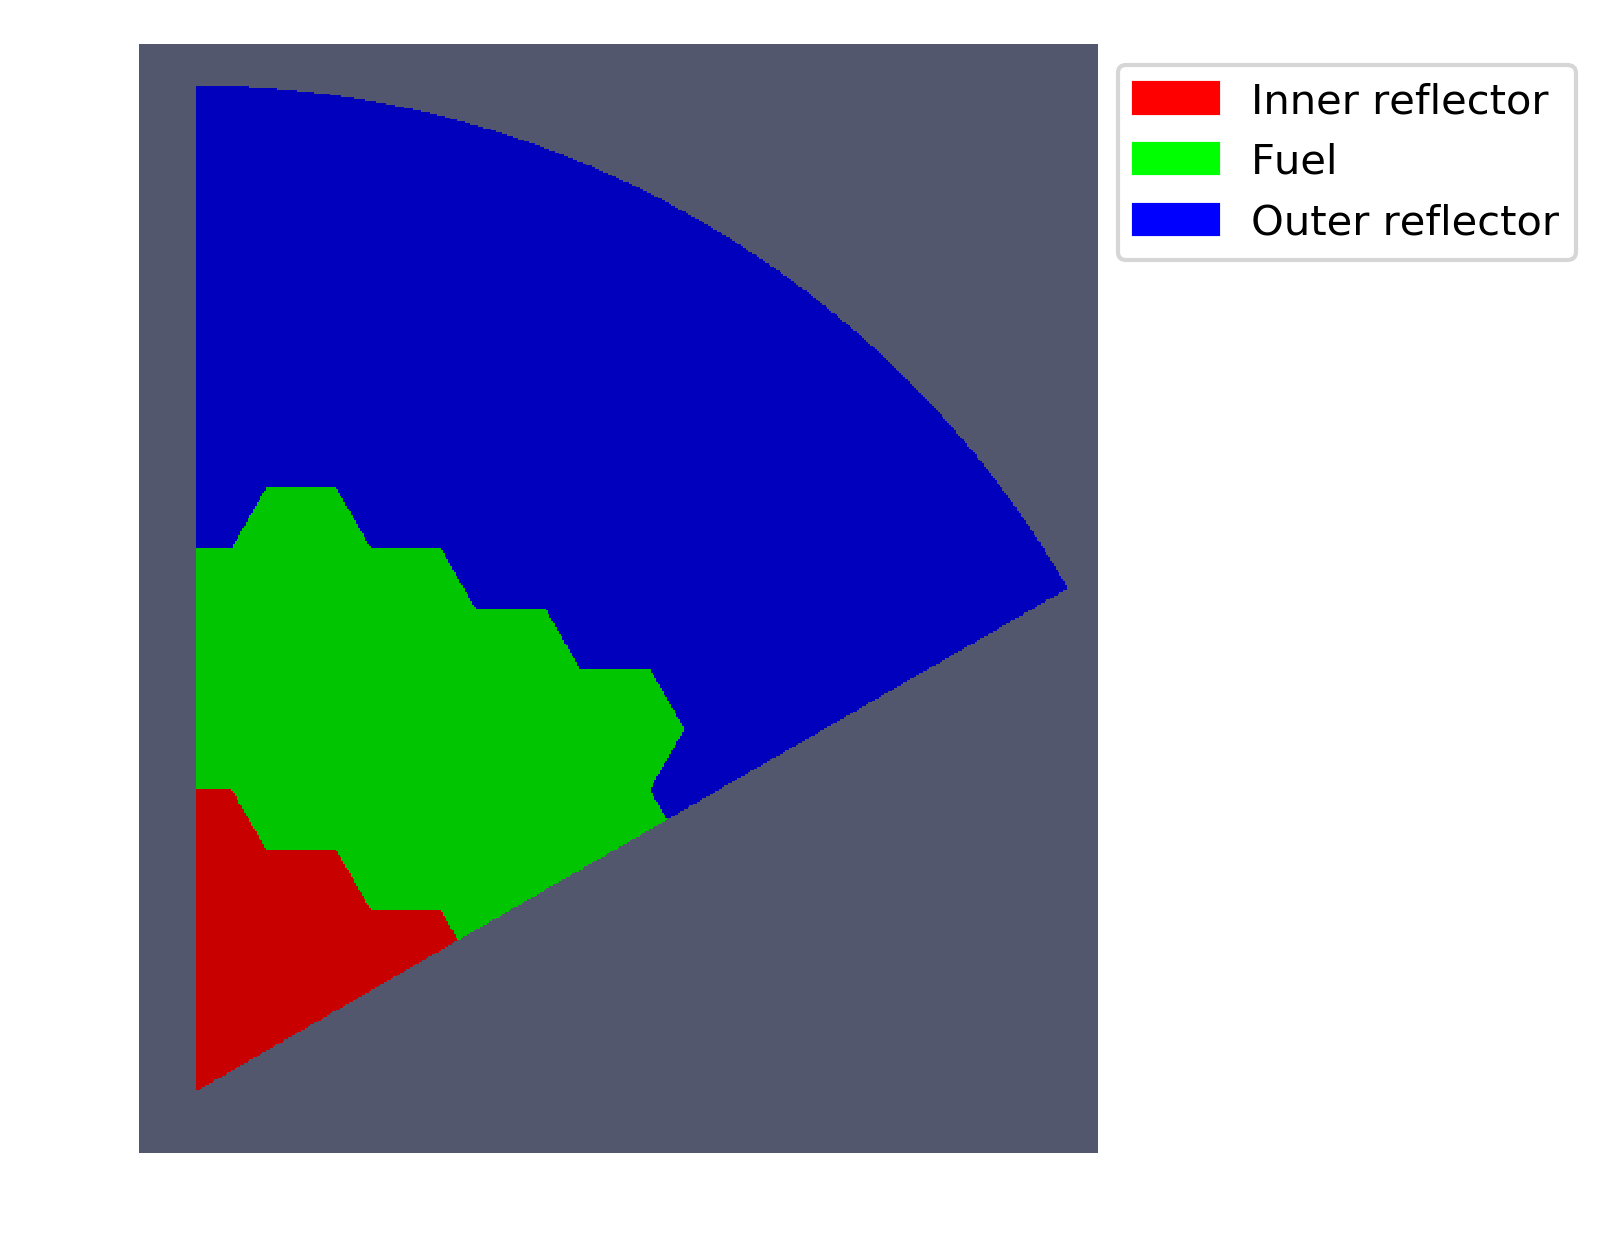
\includegraphics[width=0.42\textwidth]{figures-neutronics/3D-fullcore-60-homo-meshB2}
    }
	\hfill
  \caption{MHTGR-350 full-core model layout.}
	\label{fig:fullcoremodel}
\end{figure}

Moltres model mesh had 3.0 $\times 10^5$ elements and 1.60 $\times 10^5$ nodes.
The diffusion calculations had 1.60 $\times 10^5$ \glspl{DoF} per energy-group and a total of 2.4 $\times 10^6$ DoFs.
The Moltres input files set an eigenvalue and flux convergence tolerance of 10$^{-8}$.

% Keff
% This study compares the \gls{Keff}, the power distribution, and the flux shape and magnitude in different zones of the reactor calculated by Serpent and Moltres.
This study compares the \gls{Keff} and the radial power distribution of the reactor calculated by Serpent and Moltres.
Table \ref{tab:full-keff} exhibits the \gls{Keff} calculated by Serpent and Moltres.
The differences between the eigenvalues calculated by Moltres and Serpent are smaller than 300 pcm.

\begin{table}[htbp!]
  \centering
  \caption{Comparison between Serpent and Moltres-derived eigenvalues.}
  \begin{tabular}{cccc}
  \toprule
  Temperature [K] & Serpent	& Moltres  & $\Delta \rho$ [pcm] 	\\
  \midrule
			 600  	    & 1.10869 $\pm$ 0.00006  & 1.11150	 &	228		\\
			1200 	      & 1.06138 $\pm$ 0.00006  & 1.06468	 &	292   \\
  \bottomrule
  \end{tabular}
  \label{tab:full-keff}
\end{table}

% Power distribution
Figures \ref{fig:fullcore-600-power} and \ref{fig:fullcore-1200-power} show Serpent and Moltres radial power distributions.
Figures \ref{fig:fullcore-600-power-b} and \ref{fig:fullcore-1200-power-b} display the relative difference between Serpent and Moltres radial power distributions.
The largest relative difference is in the middle ring, and it is 6.2\% and 5.8\% MW for 600K and 1200K, respectively.
The negative values in the figures indicate that Moltres' power density is larger than Serpent's in the inner and outer rings, whereas it is lower in the middle ring, overall.

%Power distribution at 600K
\begin{figure}[htbp!]
	\centering
    \subfloat[Serpent radial power distribution.]{
        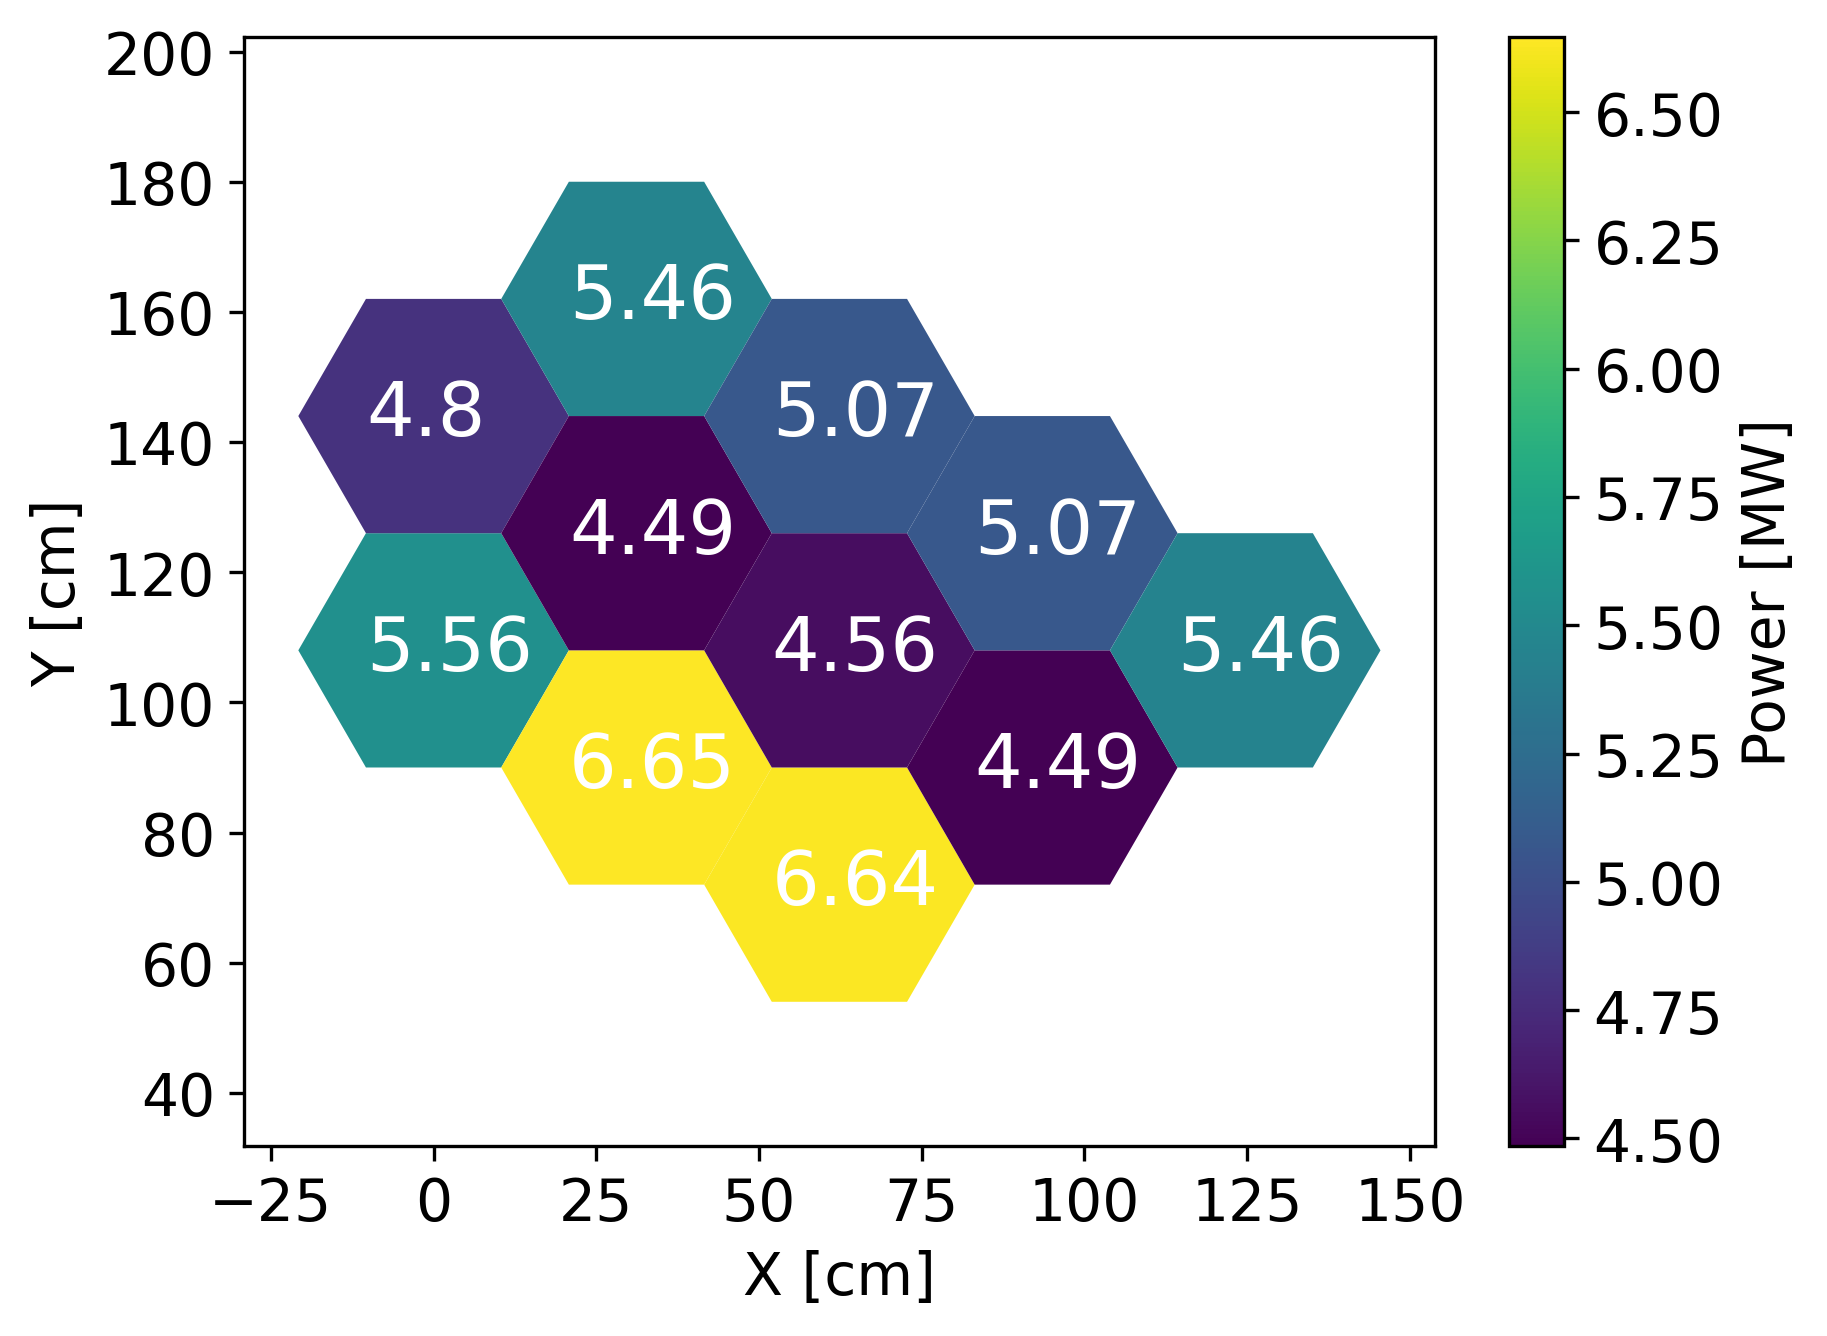
\includegraphics[width=0.45\textwidth]{figures-neutronics/serpent26G-600-power}
    }
    \subfloat[Relative difference between Serpent and Moltres radial power distributions. \label{fig:fullcore-600-power-b}]{
        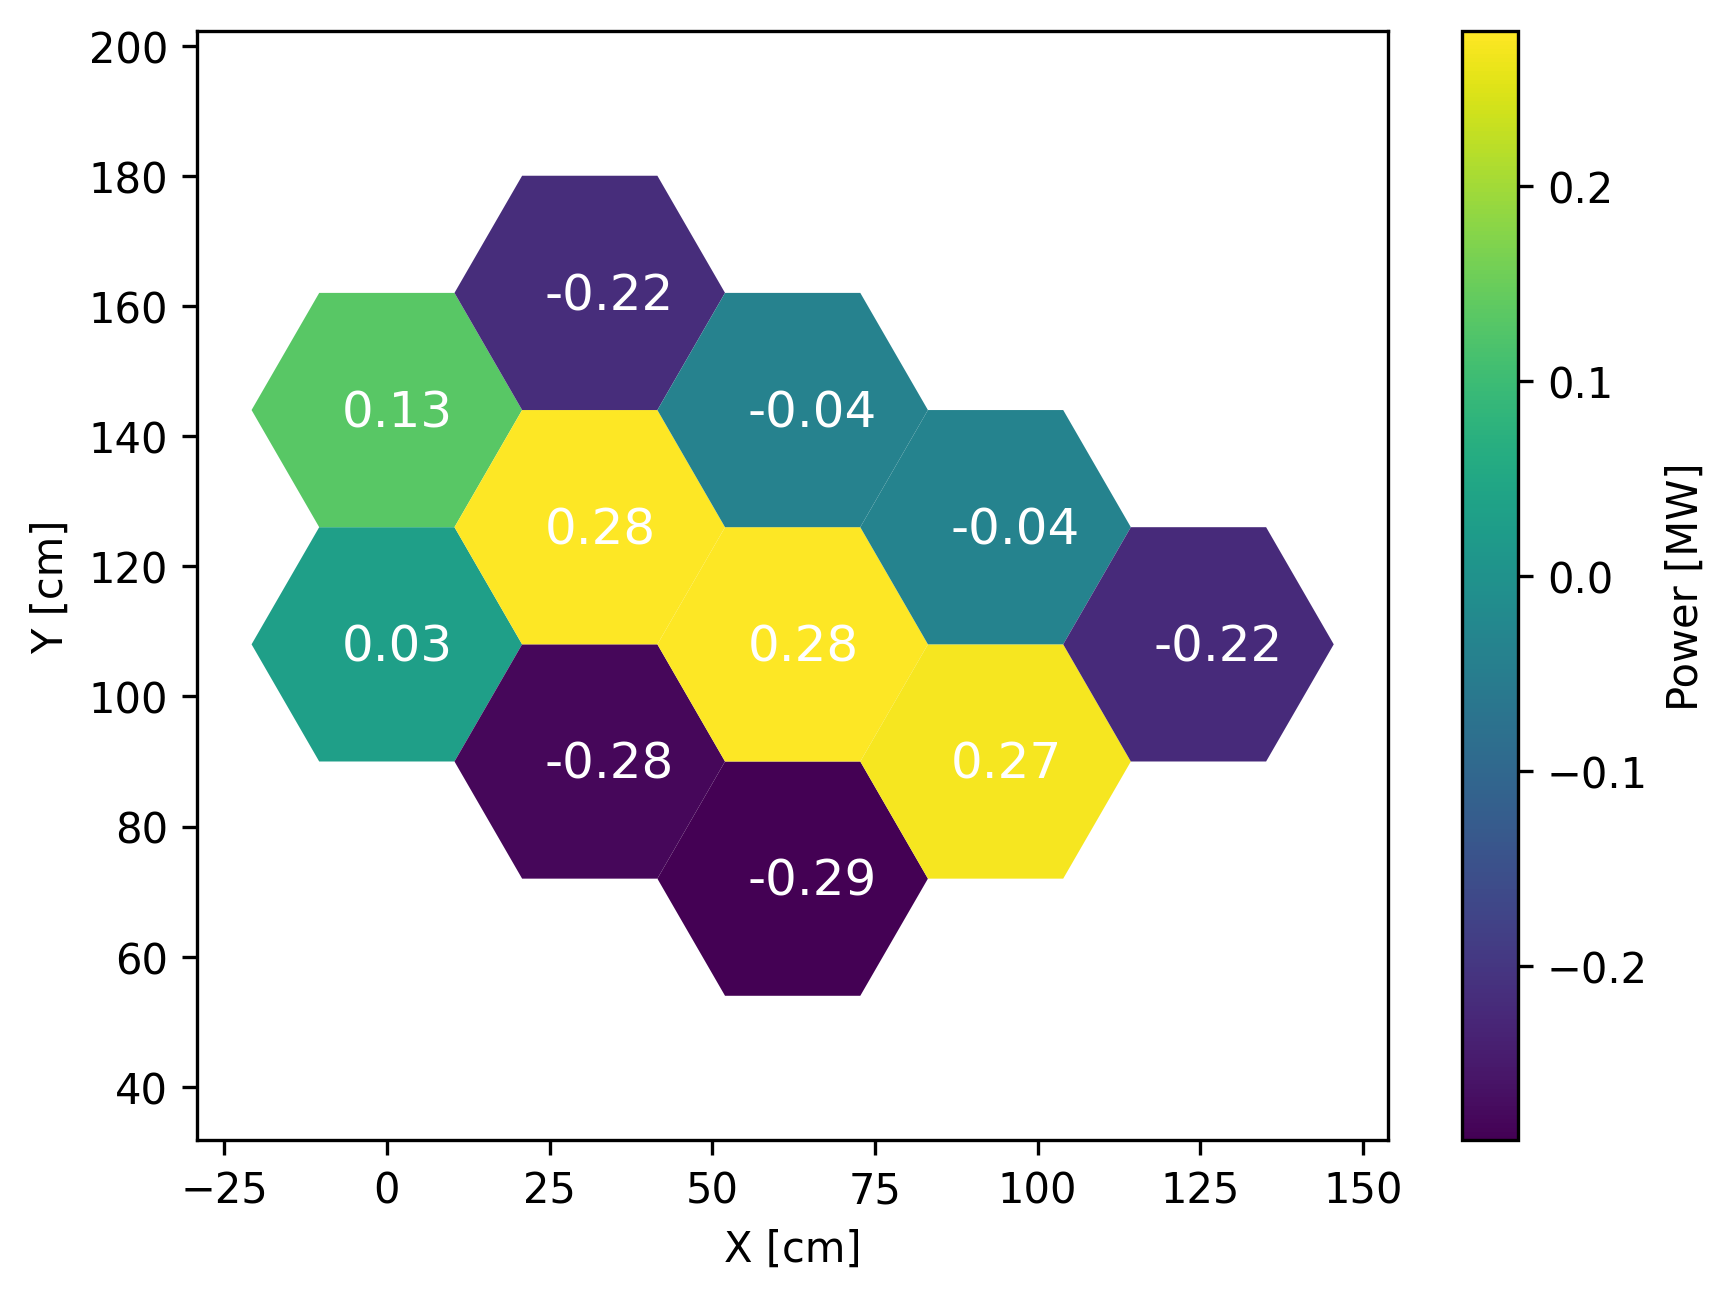
\includegraphics[width=0.45\textwidth]{figures-neutronics/serpent-moltres-600-error}
    }
	\hfill
	\caption{Comparison of the MHTGR-350 radial power distribution at 600 K calculated by Serpent and Moltres.}
	\label{fig:fullcore-600-power}
\end{figure}

%Power distribution at 1200K
\begin{figure}[htbp!]
	\centering
    \subfloat[Serpent radial power distribution.]{
        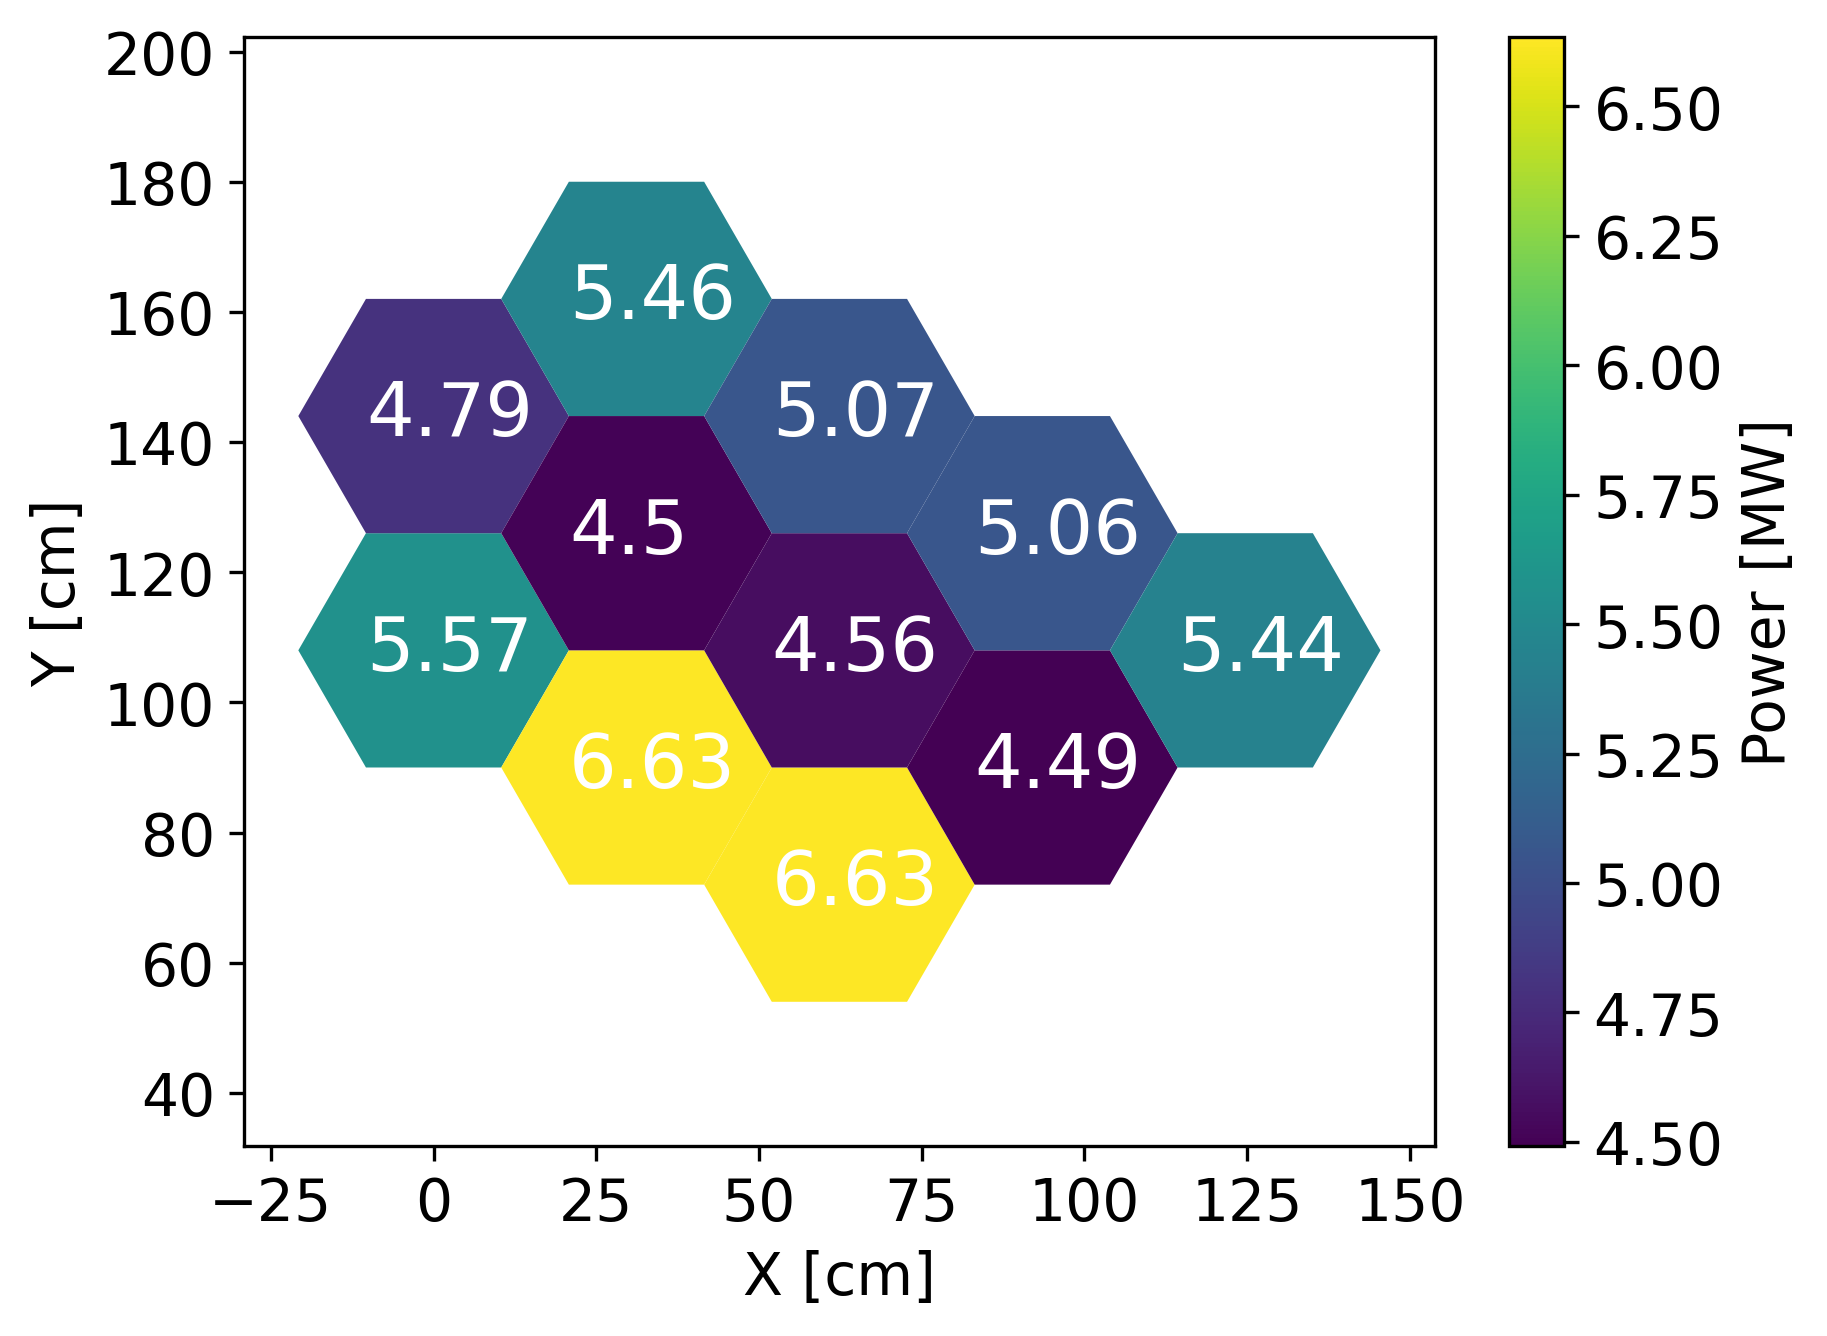
\includegraphics[width=0.45\textwidth]{figures-neutronics/serpent26G-1200-power}
    }
    \subfloat[Relative difference between Serpent and Moltres radial power distributions. \label{fig:fullcore-1200-power-b}]{
        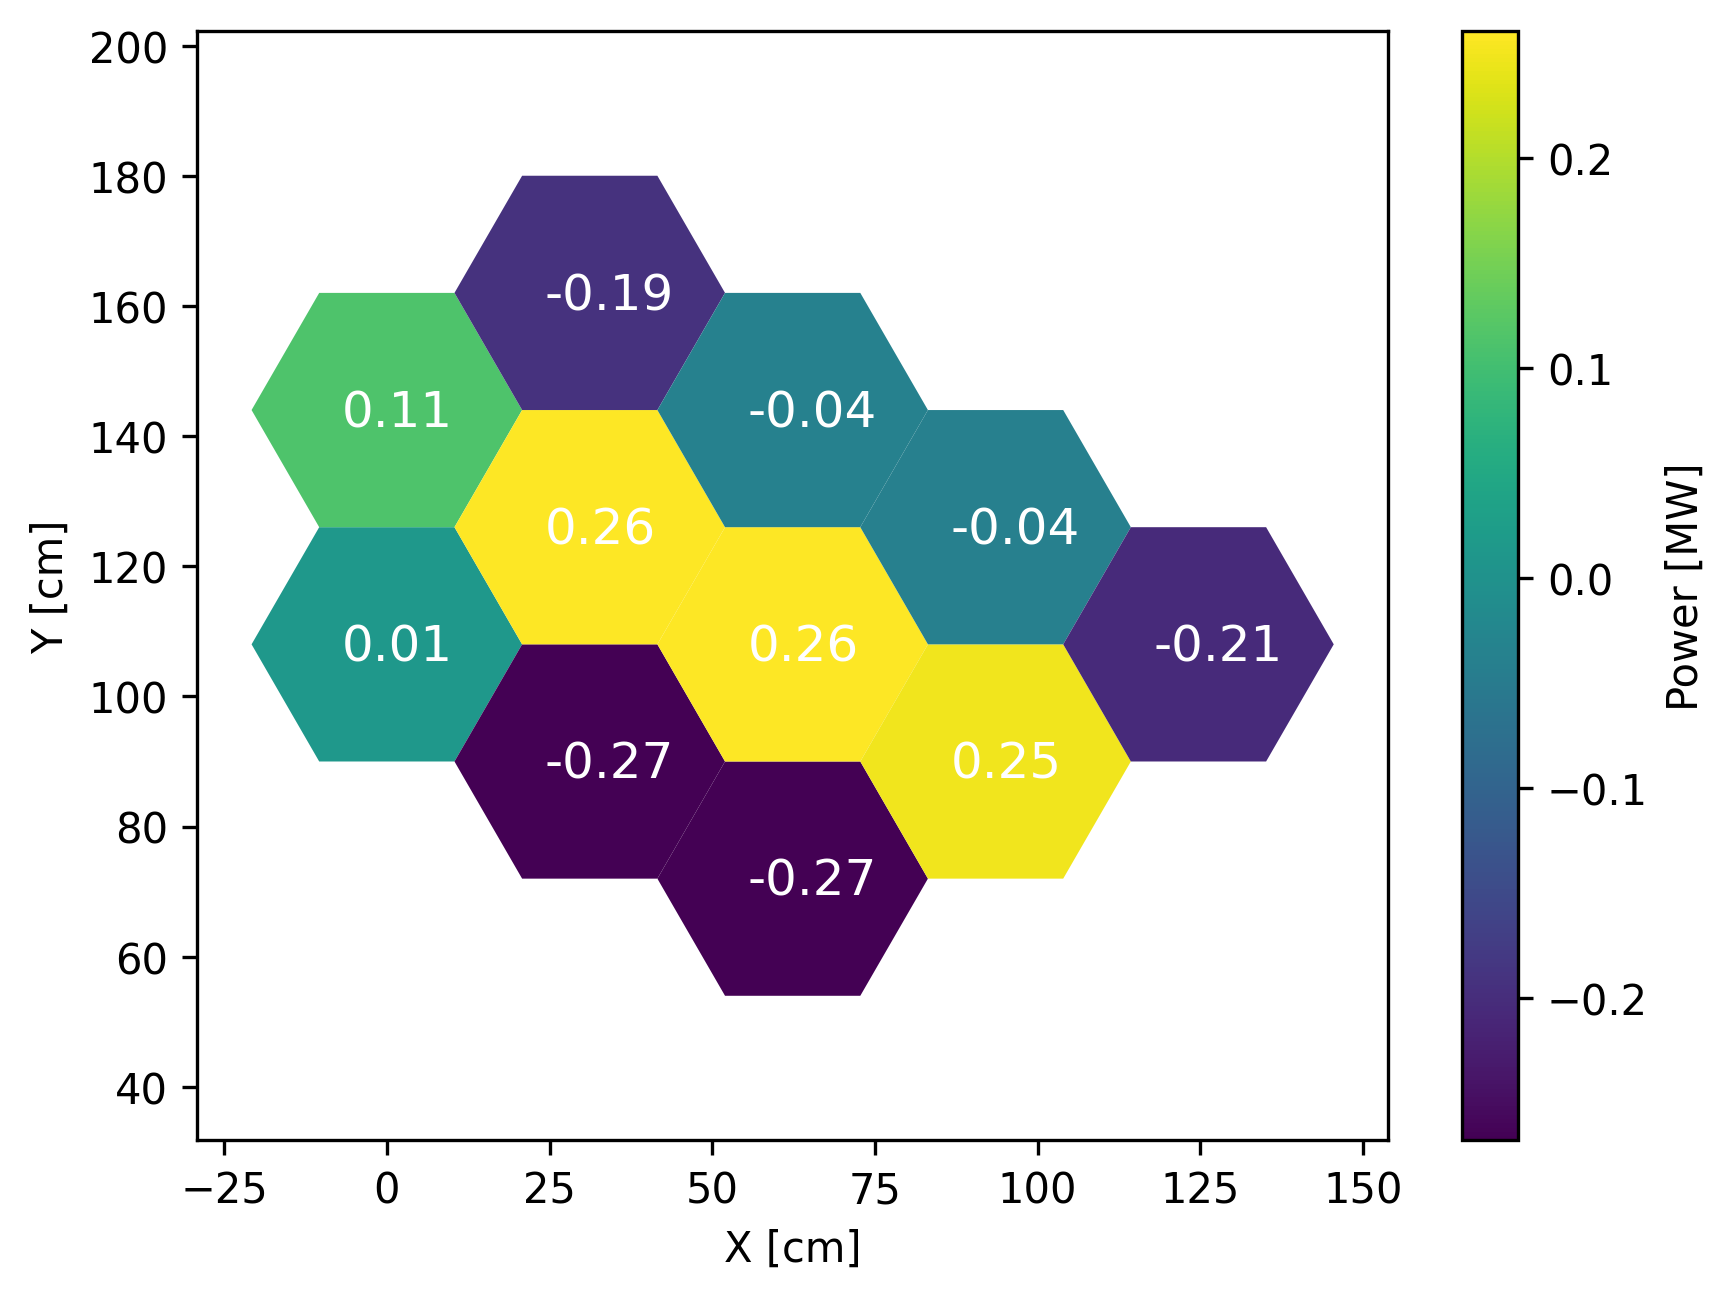
\includegraphics[width=0.45\textwidth]{figures-neutronics/serpent-moltres-1200-error}
    }
	\hfill
	\caption{Comparison of the MHTGR-350 radial power distribution at 1200 K calculated by Serpent and Moltres.}
	\label{fig:fullcore-1200-power}
\end{figure}

% Detectors
% Figure \ref{fig:fullcore-detectors} shows the neutron flux in axial and radial flux detectors in arbitrary regions of the reactor.
% Serpent simulation's axial detector has the volume of a fuel column, while the radial detector has a 2$^{\circ}$-opening and a fuel assembly height.
% Both the Serpent and Moltres radial detector's axial location was the middle of the active core's height.

% \begin{figure}[htbp!]
% 	\centering
%     \subfloat[Flux detectors in Serpent model. 1- Axial detector has the volume of a fuel column. 2- Radial detector has a 2$^{\circ}$-opening and a fuel assembly height.]{
%         % 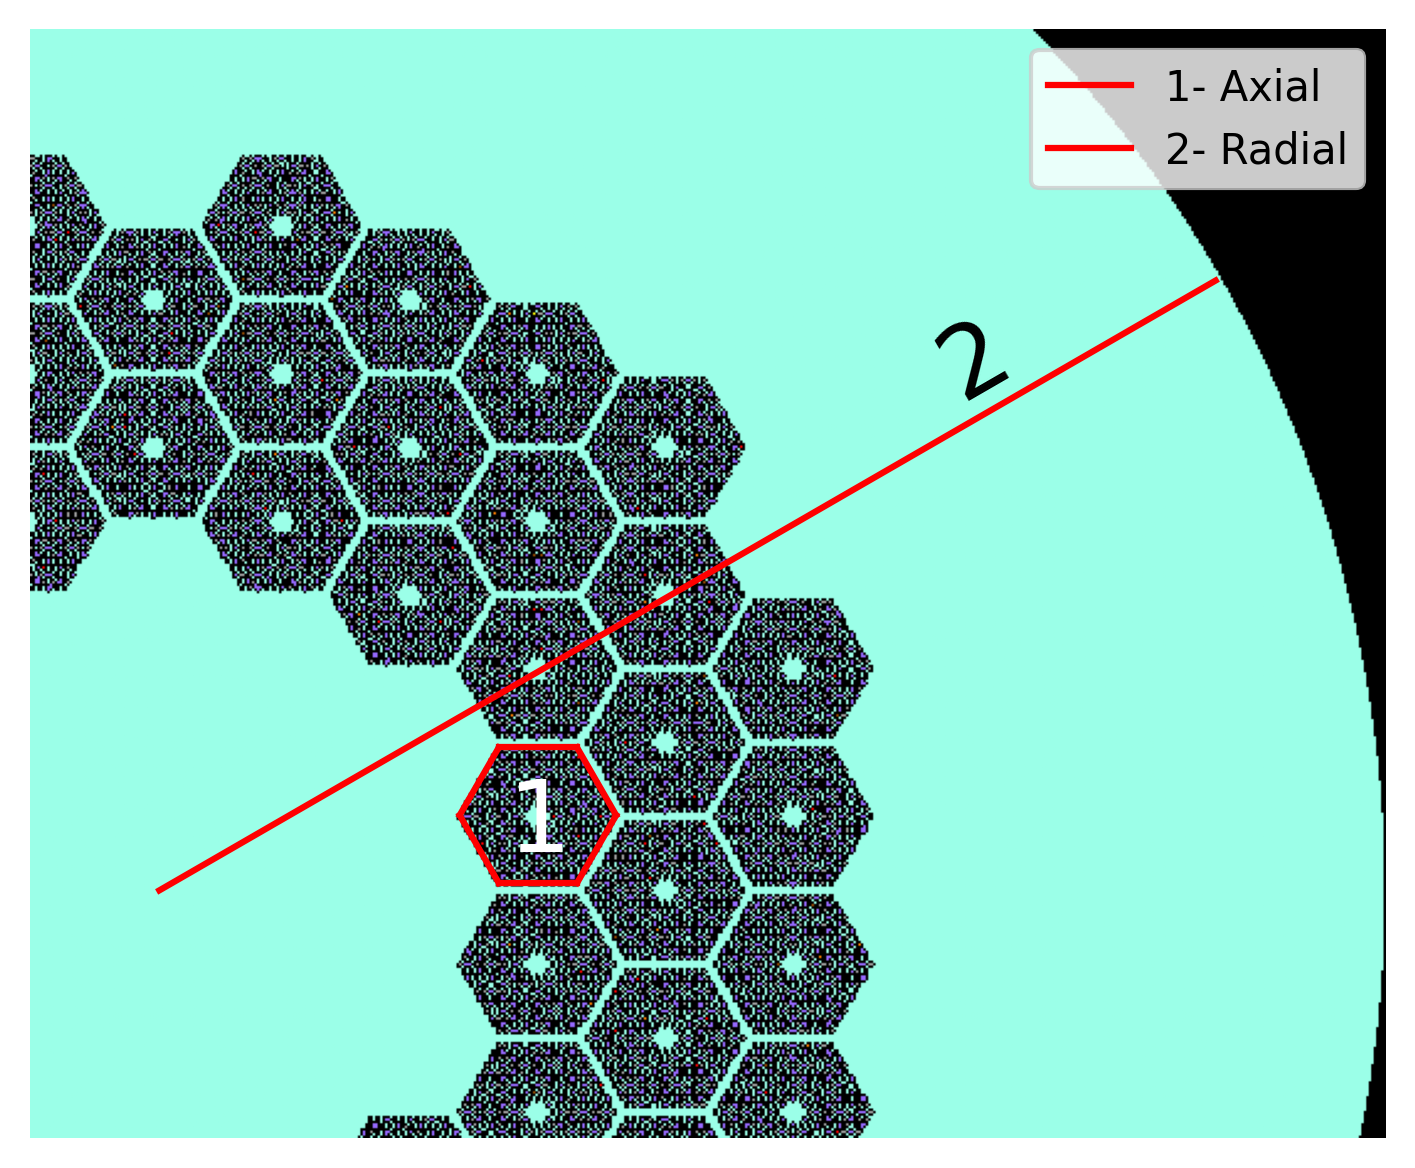
\includegraphics[width=0.52\textwidth]{figures-neutronics/oecd-fullcore-detectorsC}
%         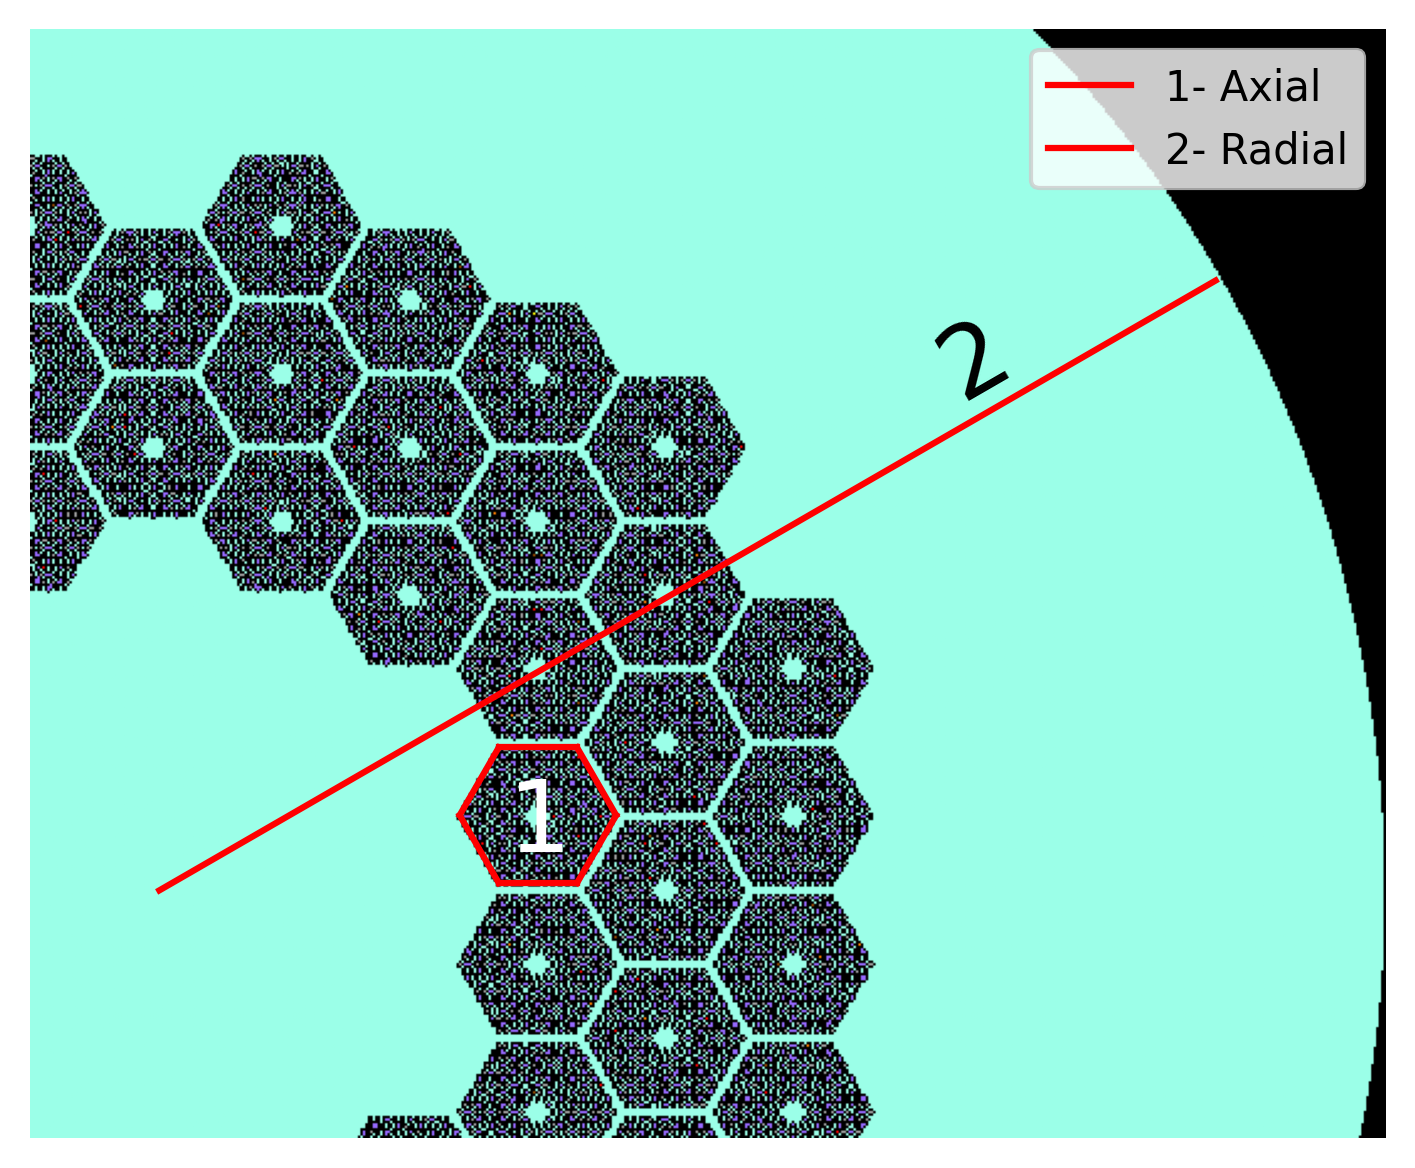
\includegraphics[width=0.52\textwidth]{figures-neutronics/oecd-fullcore-detectorsC}
%     }
% 	\hfill
%     \subfloat[Flux detectors in Moltres model. Axial detector computes the flux over the line 'Axial', corresponding to the centerline of the fuel column. Radial detector computes the flux over the line 'Radial'.]{
%         % 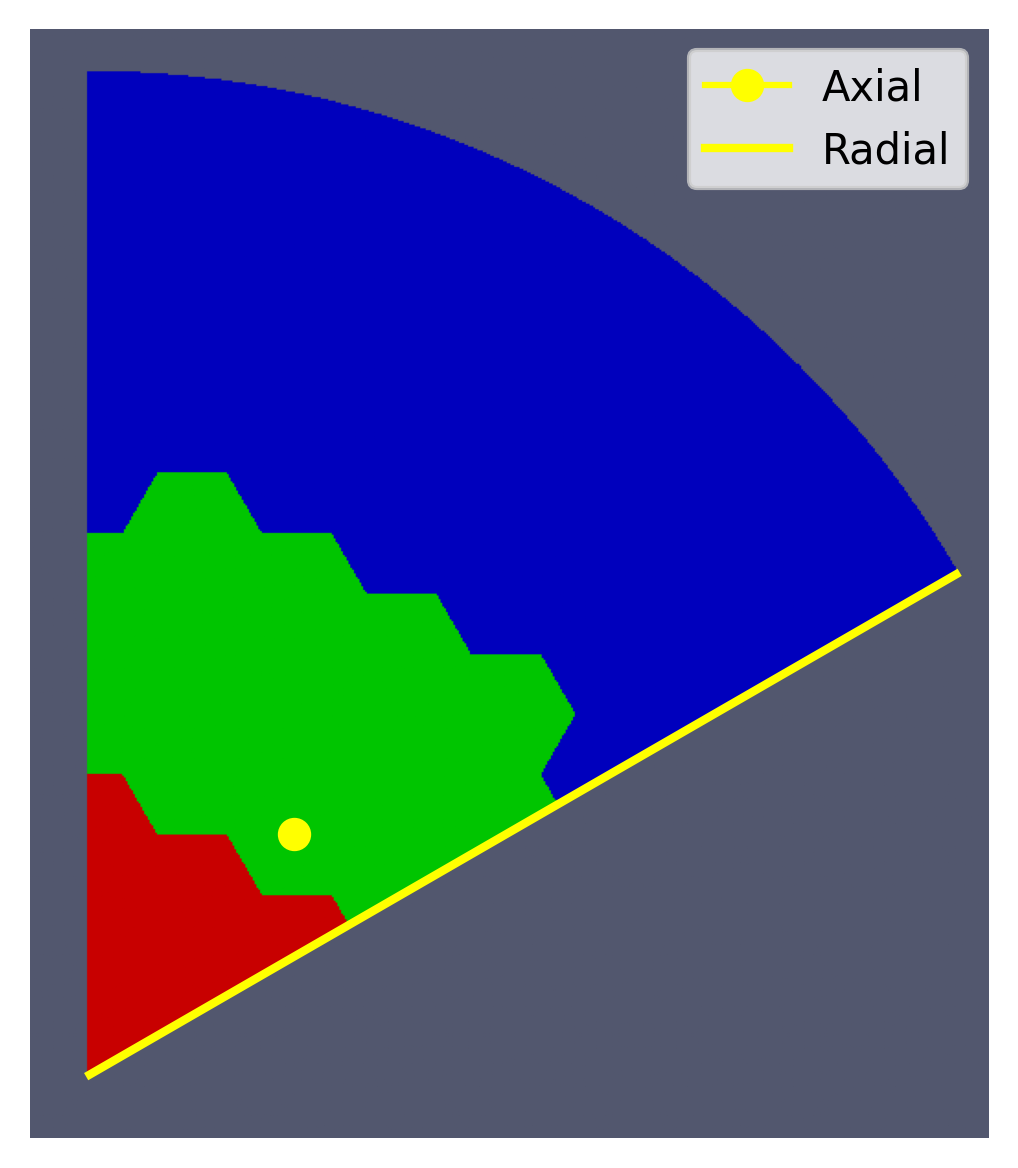
\includegraphics[width=0.37\textwidth]{figures-neutronics/3D-fullcore-60-detectors2}
%         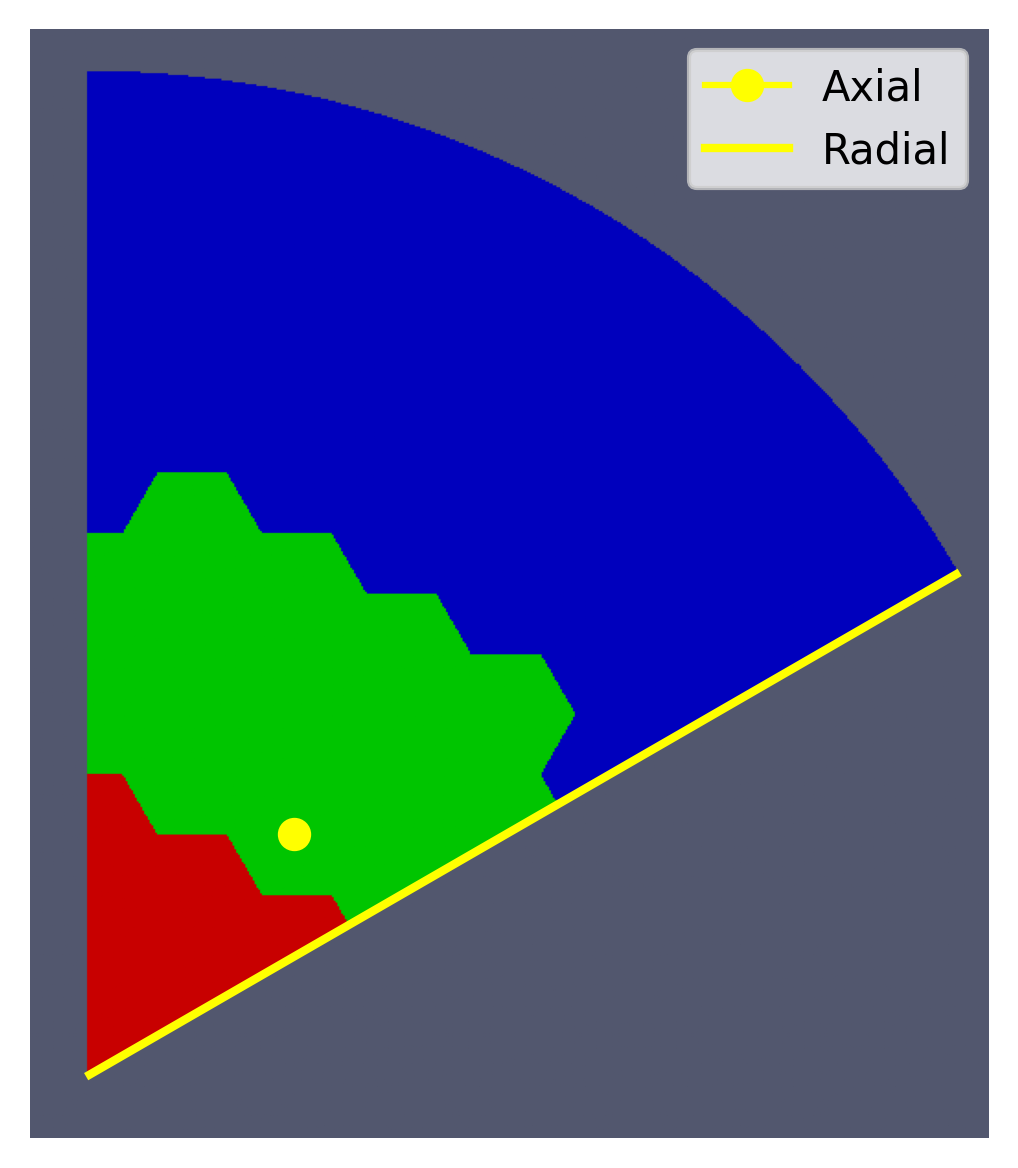
\includegraphics[width=0.37\textwidth]{figures-neutronics/3D-fullcore-60-detectors2}
%     }
% 	\caption{Axial view of the flux detector locations.}
% 	\label{fig:fullcore-detectors}
% \end{figure}

% The following analysis compares the flux calculated by Serpent and Moltres.
% Section \ref{sec:neut-fuelcol} analysis was able to study the difference between Serpent and Moltres' results because the fuel column problem uses reflective boundary conditions, making the radial profile relatively flat.
% % Consequently, Serpent flux exhibits a relatively flat radial profile, and Moltres exhibits a flat radial profile.
% Given a flat radial profile, Moltres axial flux is independent of the location of the detector.
% In the full core problem, the radial profile is far from being flat, making Moltres axial flux sensitive to the detector's location.
% For this reason, the fluxes comparison remains qualitative.

% % axial flux
% Moltres simulations used 15 energy groups, and a Python script collapsed the results into three groups to facilitate the results' visualization.
% Figure \ref{fig:fullcore-600-flux} shows the axial and radial fluxes at 600K.
% The fast and epithermal fluxes in Moltres results are larger than Serpent's, while the axial thermal flux is smaller.
% % radial flux
% Serpent's radial flux present some 'noise.'
% A higher number of generations per cycle in Serpent simulations or using a detector with a larger volume would eliminate this.
% Additionally, the radial flux in Serpent reveals the location of the burnable poisons in the fuel assemblies.
% This diffusion simulation fails to capture such localized effects as the group constants are homogeneous in the fuel assembly.
% The fast radial flux in Moltres results is larger than Serpent's, while the radial epithermal and thermal fluxes have almost the same magnitudes.
% Figure \ref{fig:fullcore-1200-flux} display the fluxes at 1200K, which differ from the 600K case.
% Still, the 1200K case exhibits the same behavior for both axial and radial fluxes.
% Overall, Moltres and Serpent fluxes are comparable in magnitude and shape.

% % Flux at 600K
% \begin{figure}[htbp!]
%   \centering
%     \subfloat[Comparison of the axial flux.]{
%         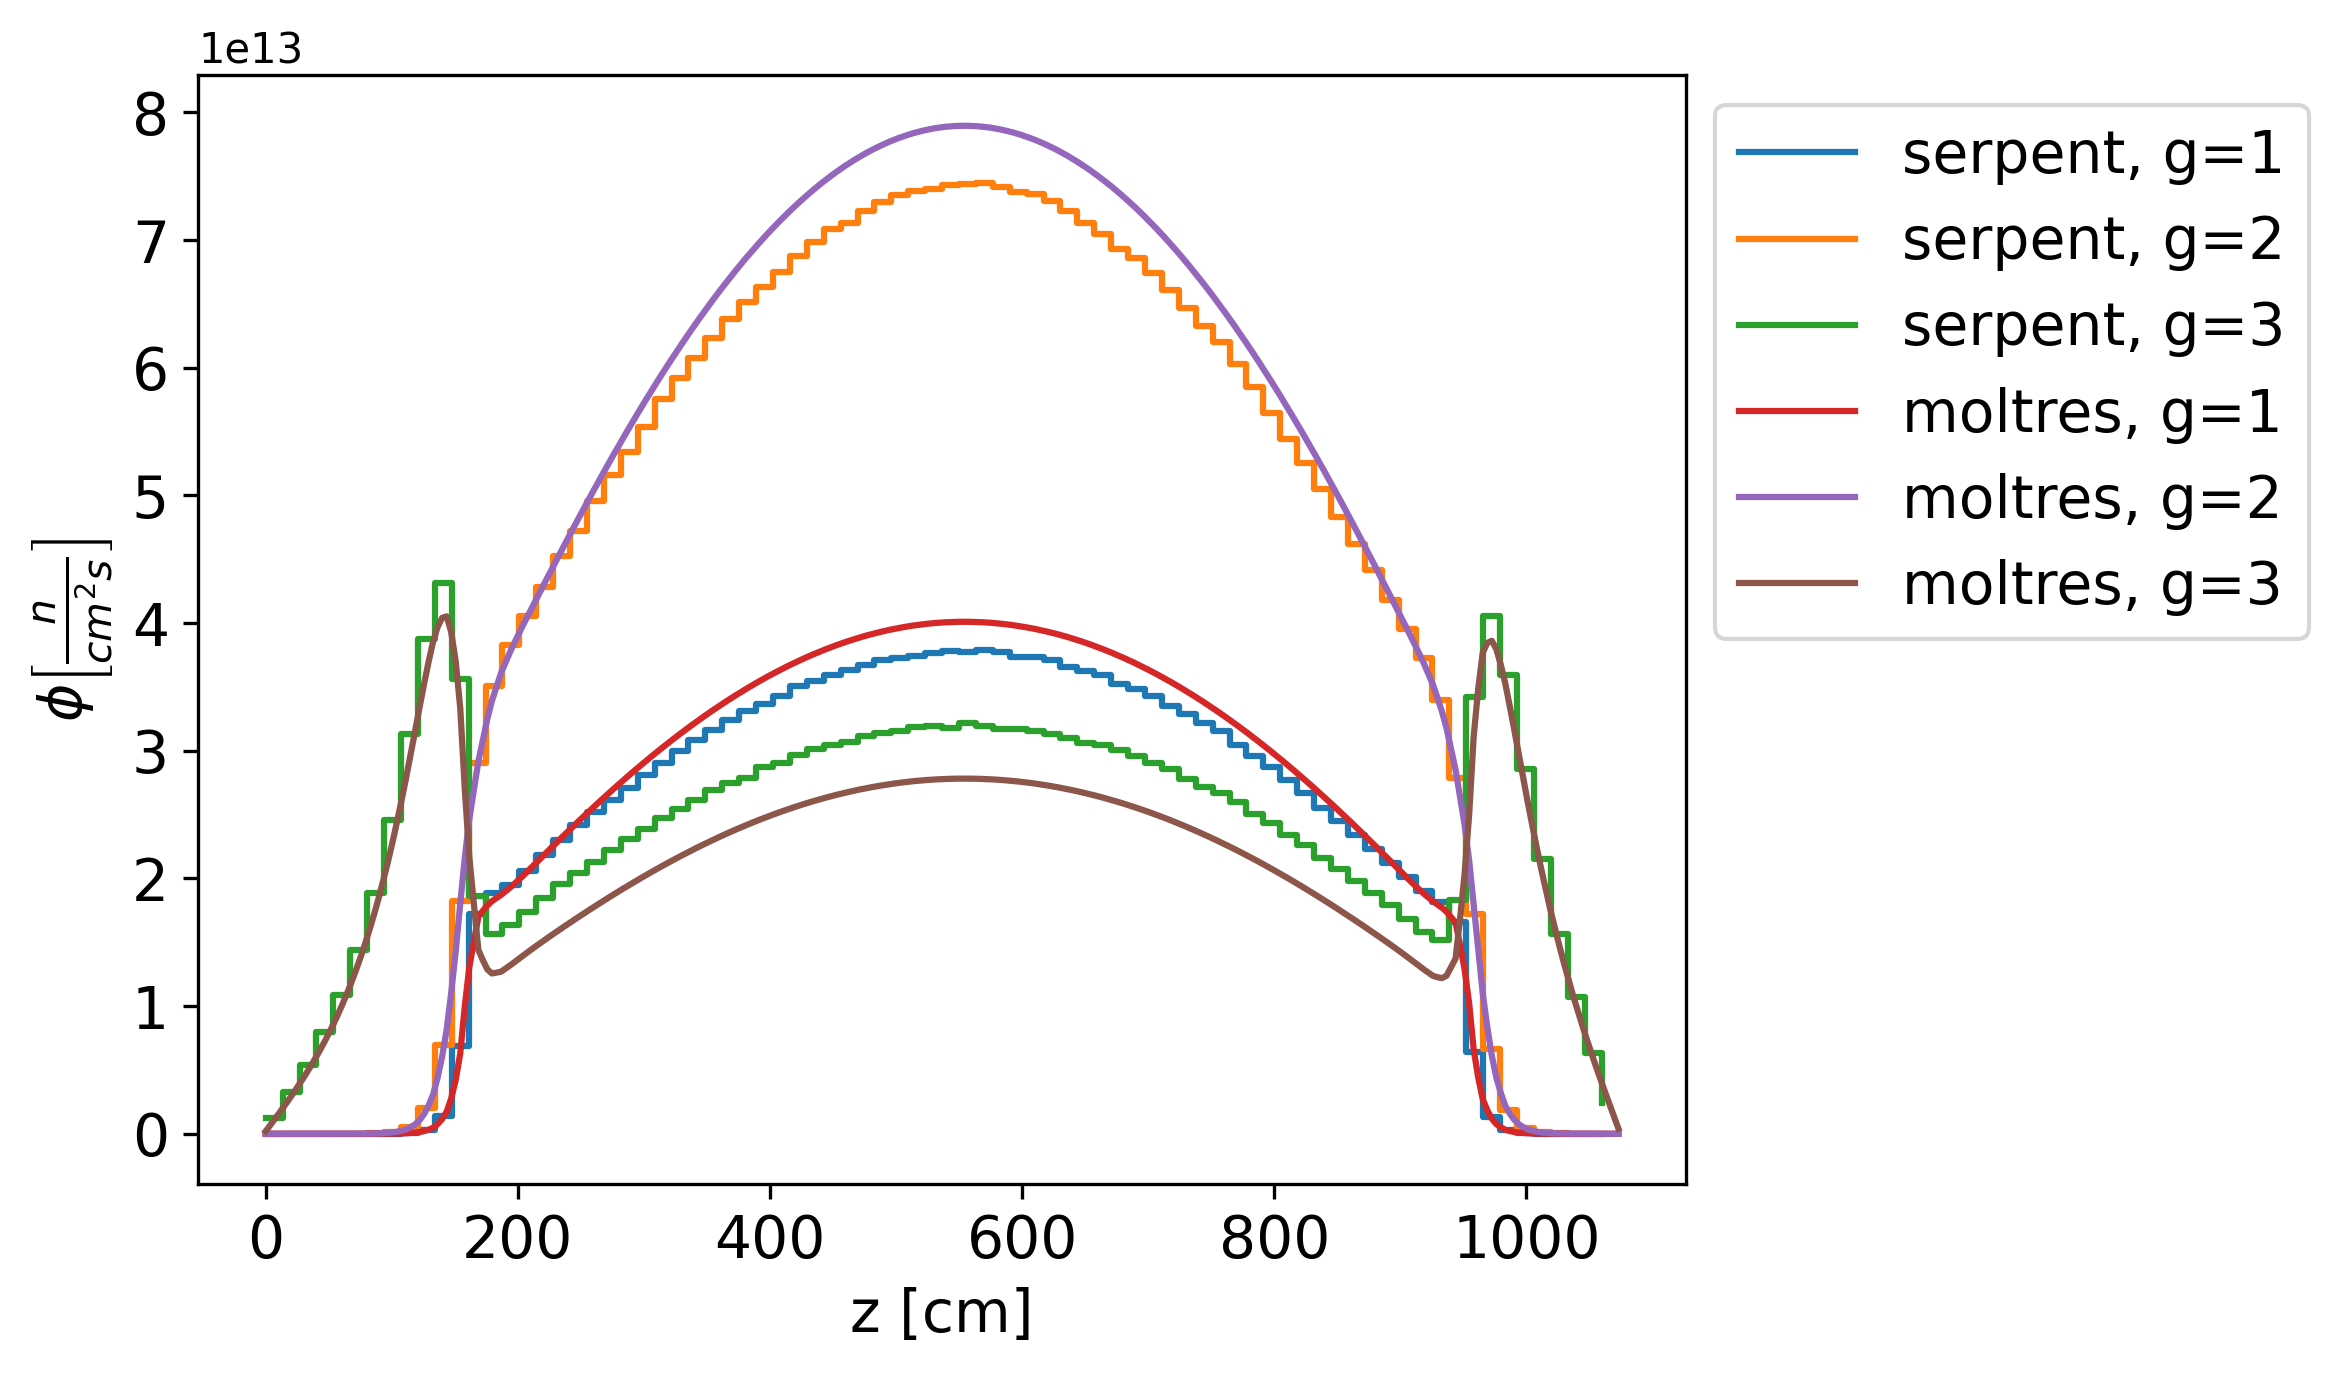
\includegraphics[width=0.45\textwidth]{figures-neutronics/serpent-moltres-axial-600}
%     }
%     \subfloat[Comparison of the radial flux.]{
%         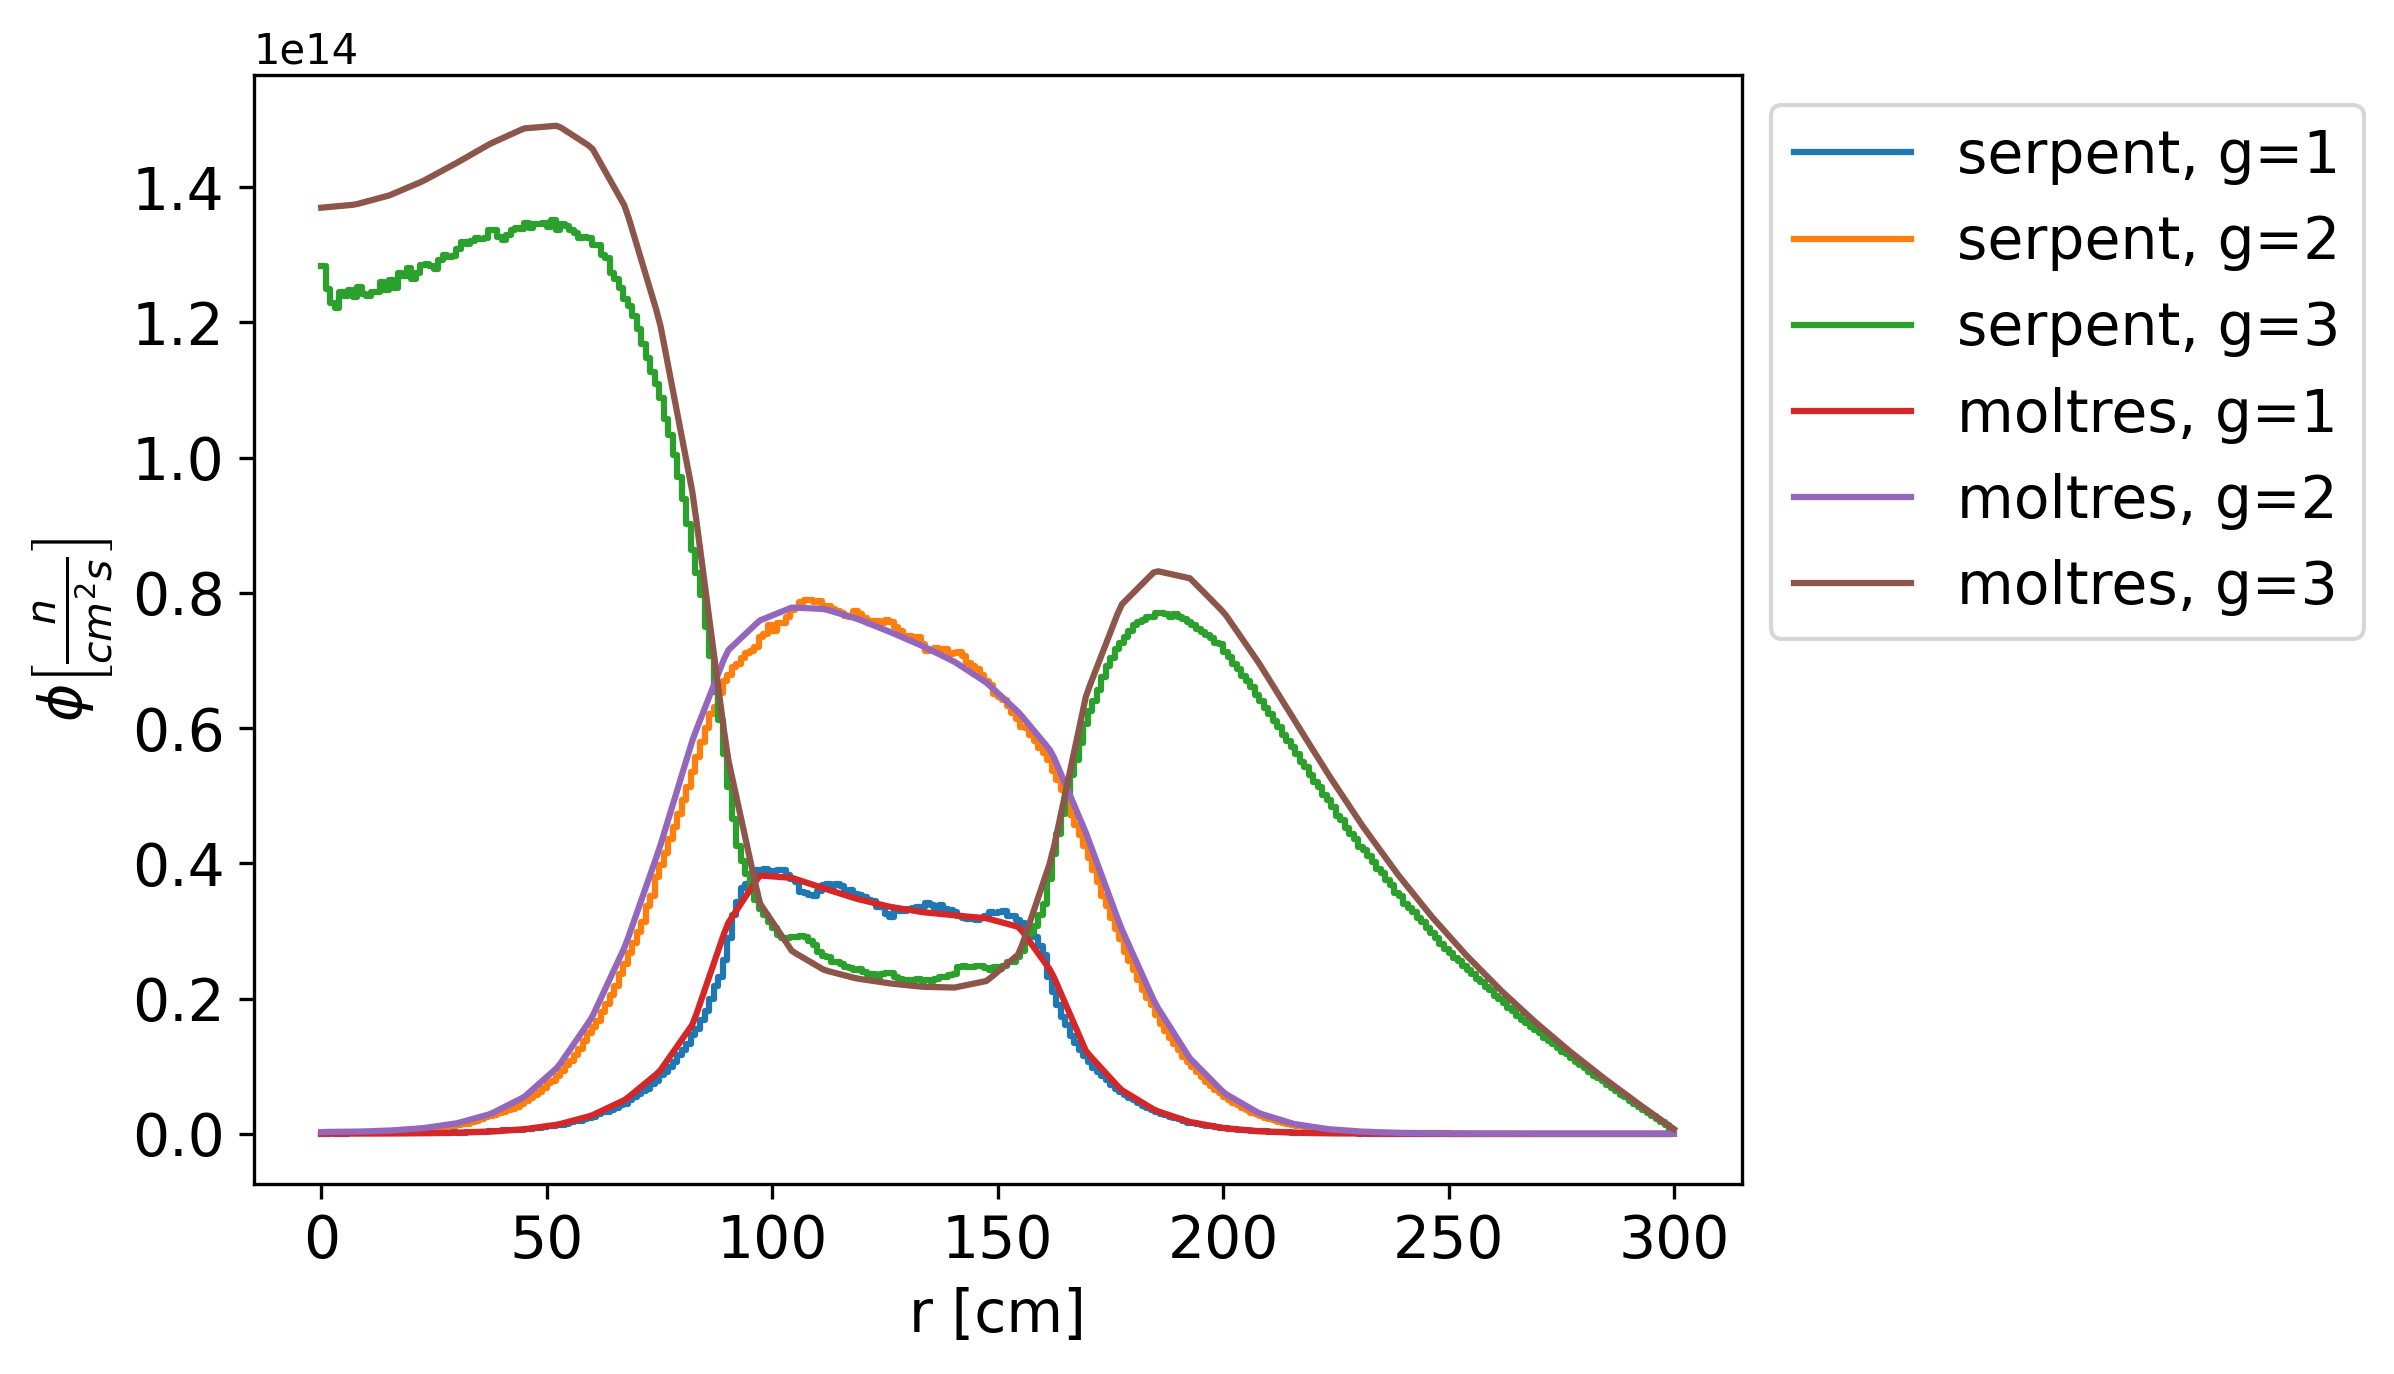
\includegraphics[width=0.45\textwidth]{figures-neutronics/serpent-moltres-radial-600}
%     }
%   \hfill
%   \caption{Comparison of the axial and radial fluxes calculated by Serpent and Moltres at 600 K.}
%   \label{fig:fullcore-600-flux}
% \end{figure}

% % Flux at 1200 K
% \begin{figure}[htbp!]
%   \centering
%     \subfloat[Comparison of the axial flux.]{
%         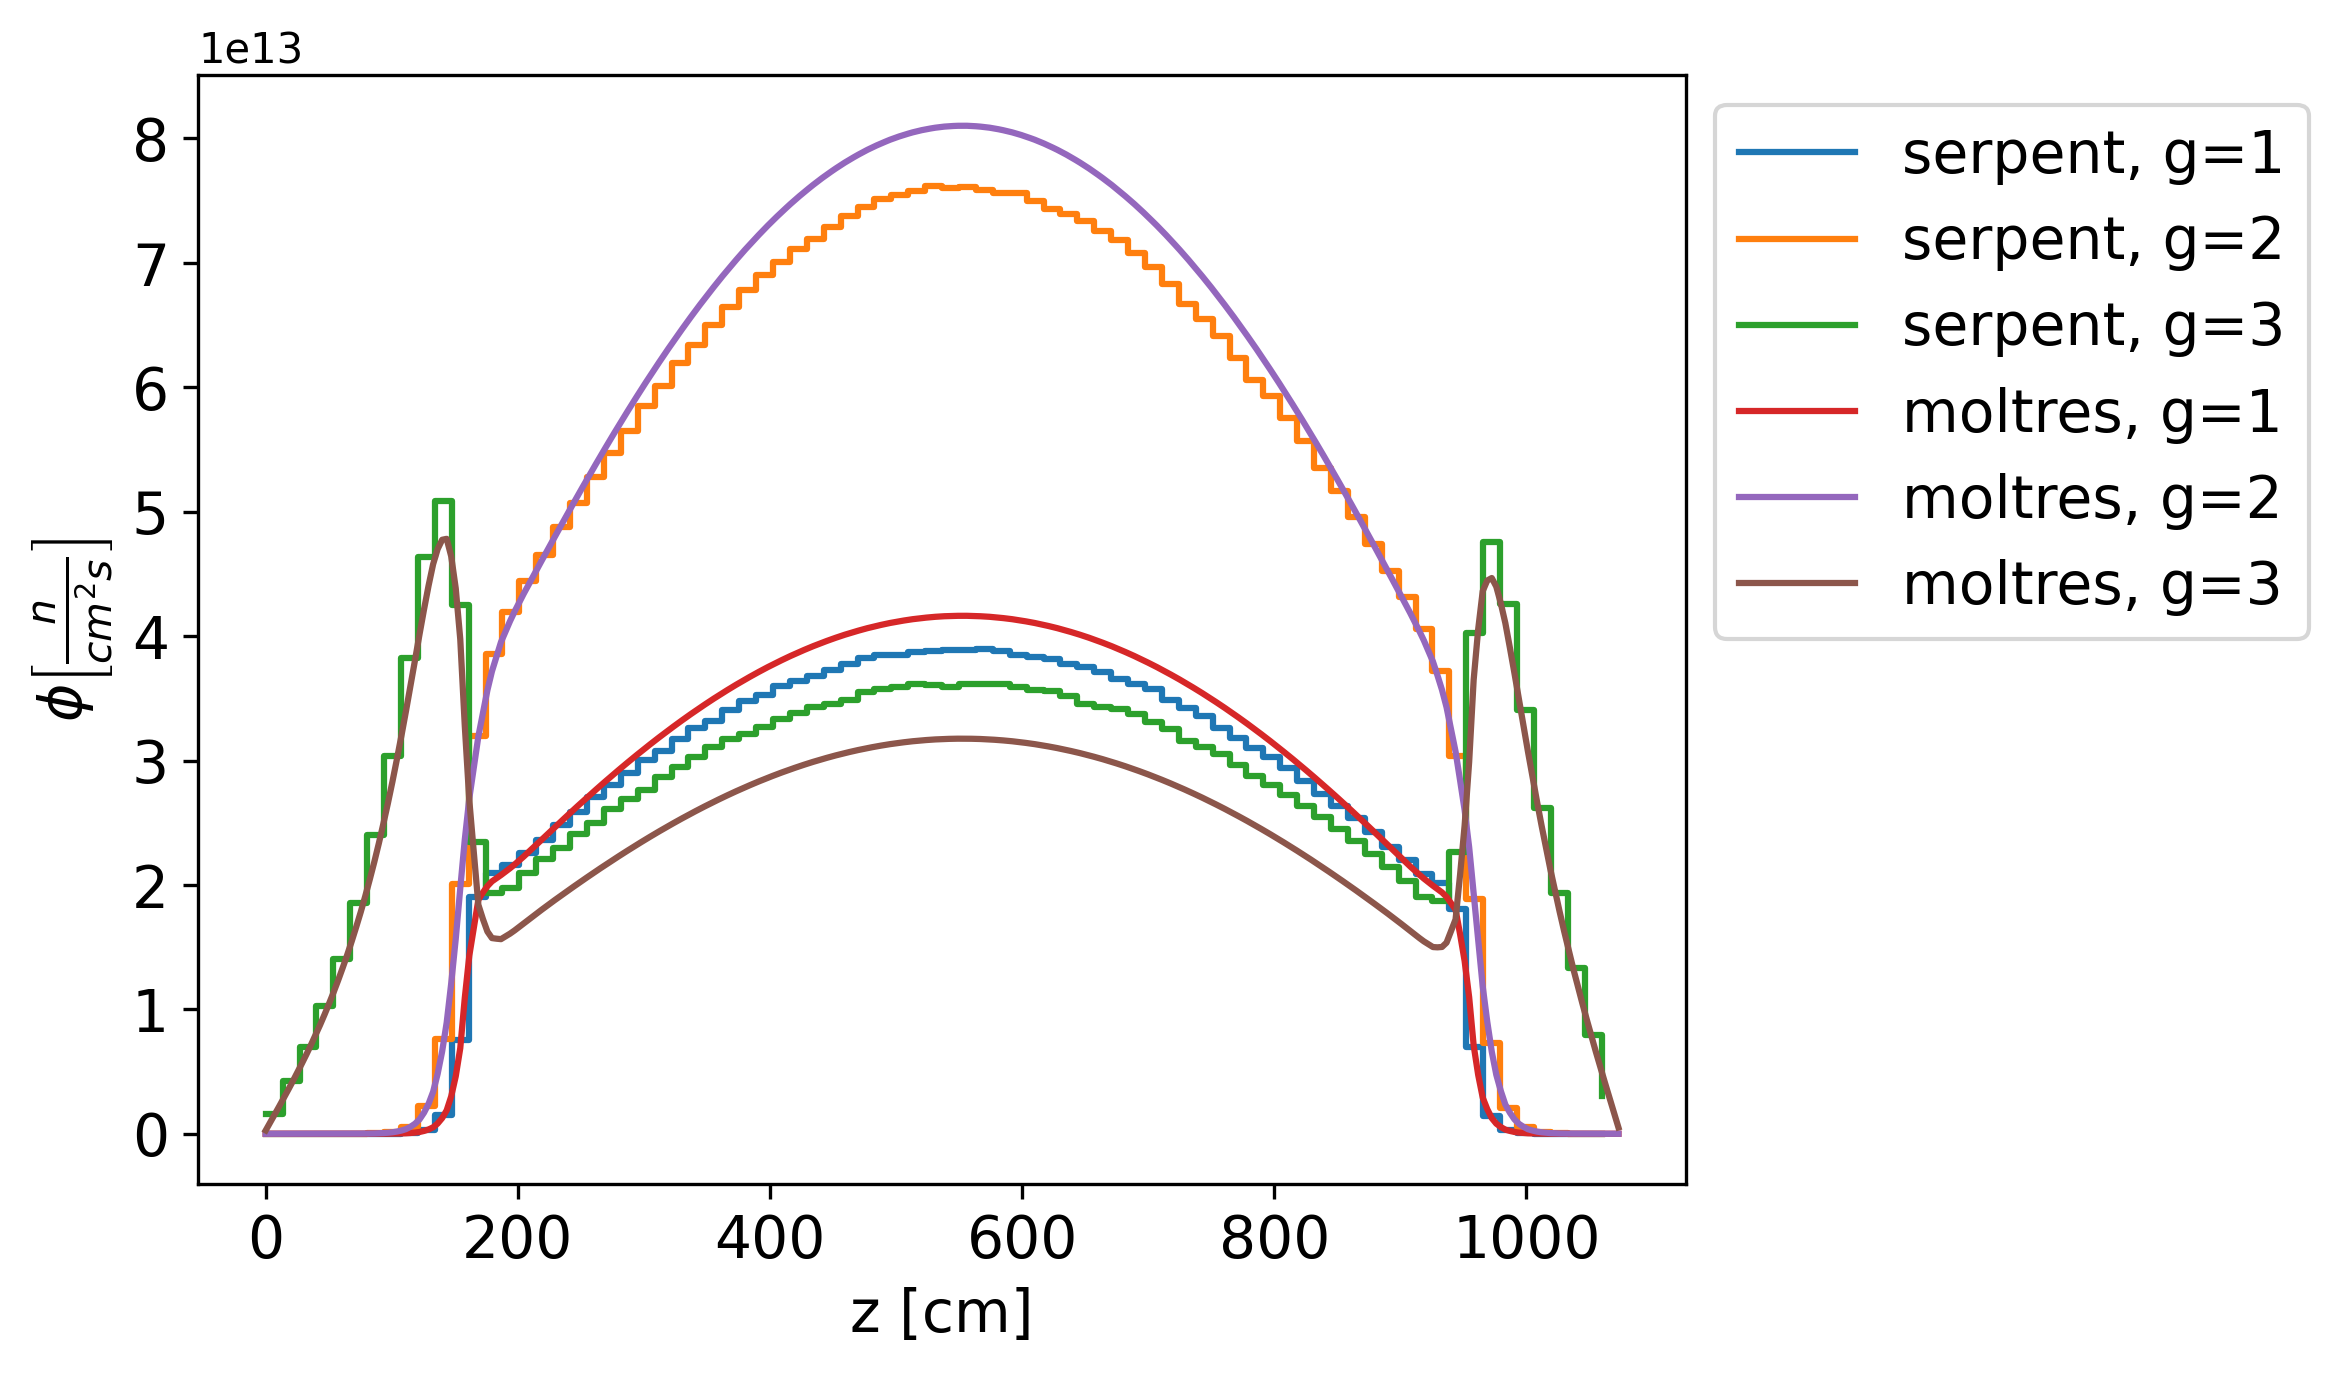
\includegraphics[width=0.45\textwidth]{figures-neutronics/serpent-moltres-axial-1200}
%     }
%     \subfloat[Comparison of the radial flux.]{
%         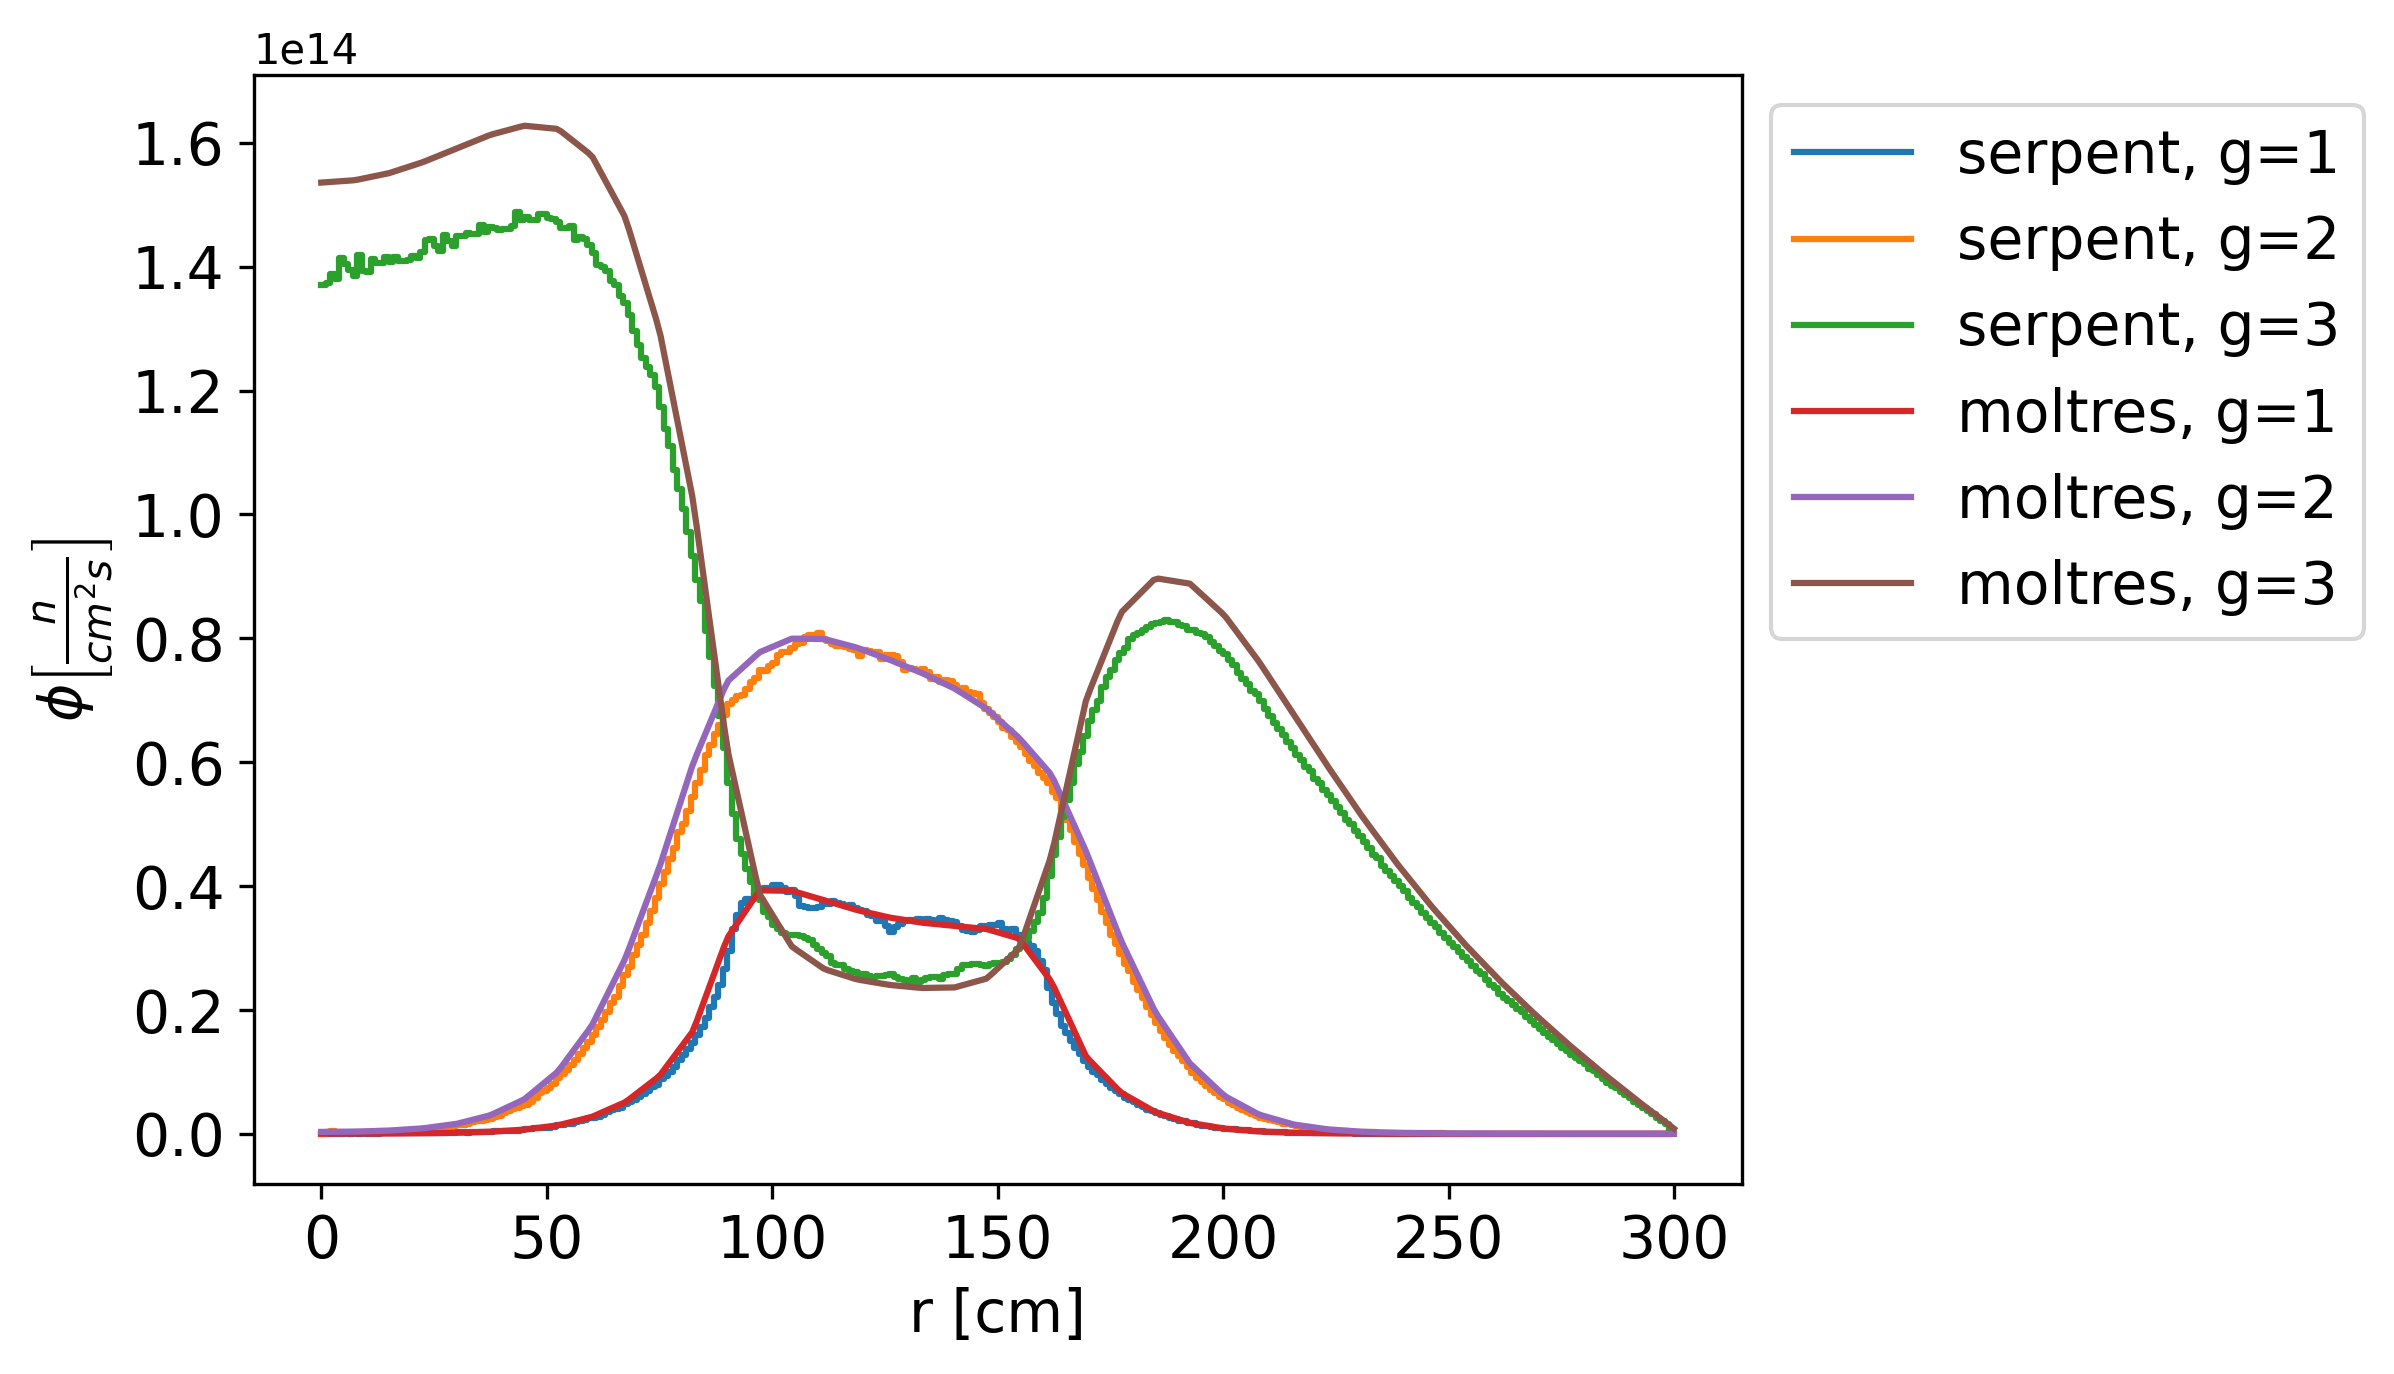
\includegraphics[width=0.45\textwidth]{figures-neutronics/serpent-moltres-radial-1200}
%     }
%   \hfill
%   \caption{Comparison of the axial and radial fluxes calculated by Serpent and Moltres at 1200 K.}
%   \label{fig:fullcore-1200-flux}
% \end{figure}


\section{OECD/NEA MHTGR-350 Benchmark: Phase I Exercise 1}
\label{sec:ph1e1}

% Exercise description
This section discusses Phase I Exercise 1 of the OECD/NEA MHTGR-350 Benchmark conducted with Moltres and compares the results with those already published \cite{oecd_nea_coupled_2020}.
The benchmark specifies the group constants required to conduct the exercise, ensuring a common dataset among various benchmark participants and allowing stand-alone neutronic comparison without thermal-fluids feedback.
The exercise requests the reporting of the global parameters: $K_{eff}$, control rod worth ($\Delta \rho_{CR}$), axial offset ($AO$), and the power distribution map \cite{oecd_nea_benchmark_2017}.
Equations \ref{eq:controlrod} and \ref{eq:ao} define $\Delta \rho_{CR}$ and $AO$
\begin{align}
    \Delta \rho_{CR} &= \frac{k_{eff, out}-k_{eff, in}}{k_{eff, out}k_{eff, in}} \label{eq:controlrod}
    \intertext{where}
    \Delta \rho_{CR} &= \mbox{control rod worth} [-] \notag \\
    k_{eff, out} &= \mbox{eigenvalue with \gls{CR} out (at position z=911.7 cm)} [-] \notag \\
    k_{eff, in} &= \mbox{eigenvalue with \gls{CR} in (at position z=99 cm)} [-] \notag
		\intertext{and}
    AO &= \frac{P_{top}-P_{bottom}}{P_{top}+P_{bottom}} \label{eq:ao}
    \intertext{where}
    AO &= \mbox{axial offset } [-] \notag \\
    P_{top} &= \mbox{total power produced in the top half core } [W] \notag \\
    P_{bottom} &= \mbox{total power produced in the bottom half core } [W]. \notag
\end{align}

The Moltres simulation modeled $1/3^{rd}$ of the reactor, shown in Figure \ref{fig:bench-mesh}, including the bottom and top reflectors.
Two hundred and thirty-two hexagonal subdomains comprised the core, for which the benchmark provides group constants.
% Table \ref{tab:mac-region} lists the six macroscopic regions that we can differentiate in the model.
The simulations required two meshes: one for the control rod out and one for the control rod in.
The control rod out simulation had 2.7 $\times 10^5$ \glspl{DoF} per energy-group, and a total of 7.0 $\times 10^6$ DoFs, while the control rod in simulation had 2.3 $\times 10^5$ \glspl{DoF} per energy-group, and a total of 5.9 $\times 10^6$ DoFs.
The Moltres input files set an eigenvalue convergence tolerance of 10$^{-8}$.

\begin{figure}[htbp!]
	\centering
	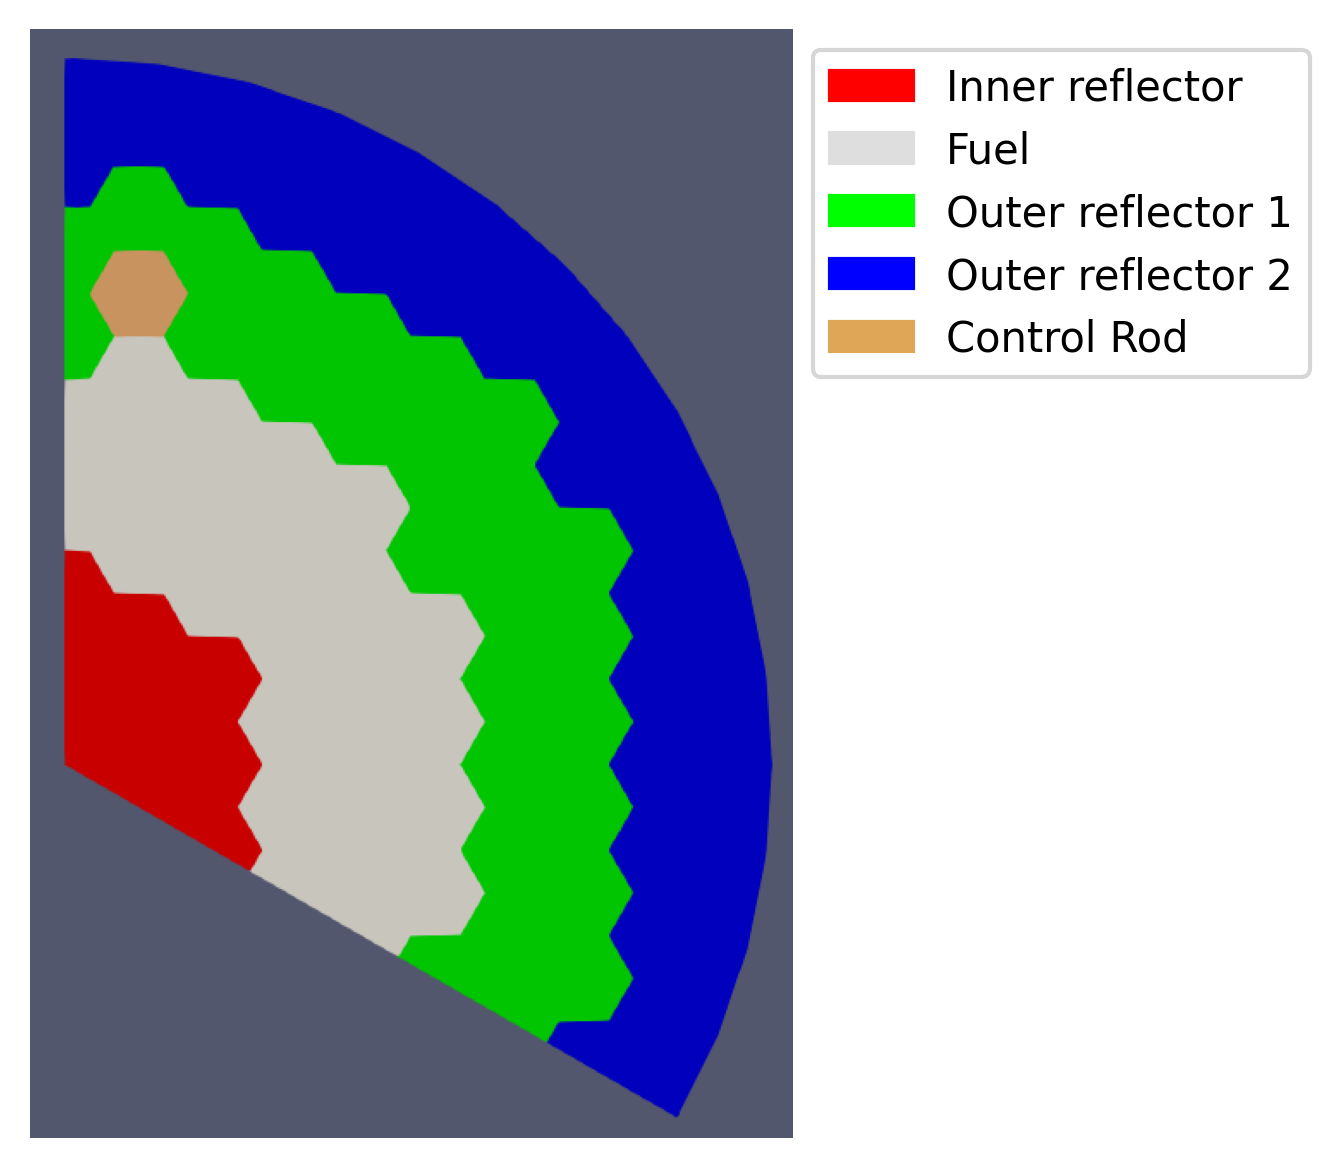
\includegraphics[width=0.55\linewidth]{figures-neutronics/oecd-fullcore-legend}
	\hfill
	\caption{Moltres model, $1/3^{rd}$ section of the MHTGR-350.}
	\label{fig:bench-mesh}
\end{figure}

% \begin{table}[htbp!]
%   \centering
%   \caption{Macroscopic regions .}
%   \label{tab:mac-region}
%   \begin{tabular}{@{}l c}
%   \toprule
%   Macroscopic region    & Subdomains     \\
%   \midrule
%   Fuel              & 1 to 220      \\
%   Bottom reflector  & 221 to 224    \\
%   Inner reflector   & 225           \\
%   Outer reflector   & 226-227       \\
%   Top reflector     & 228 to 231    \\
%   Control Rod       & 232           \\
%   \bottomrule
%   \end{tabular}
% \end{table}

The benchmark exercise specifies the group constants and a map with their location.
The benchmark definition used DRAGON-4 \cite{marleau_user_2016} to obtain the group constants from a full block configuration.
The dataset contains 26 energy groups.
The benchmark specifies the following group constants: $\Sigma_g^t$, $D_g$, $\nu\Sigma_g^f$, $\Sigma_g^f$, $\chi_g^t$, and $\Sigma_{g'\rightarrow g}^s$ (see equation \ref{eq:diffusion-eig}).
The benchmark group constants' format differs from the Moltres format, and a script handled the formatting differences.

The benchmark exercise sets periodic \glspl{BC} on the sides of the geometry; however, a memory issue did not allow for implementing those BCs in our 26-group Moltres input file.
Moltres simulations approximated the periodic BC with the reflective BC.
Section \ref{sec:bench-bcs} discusses further the use of periodic and reflective BCs.

% 4.33 h and 4.11 h
On average, the simulations took 4.22 hours using 1024 cores.
Table \ref{tab:globalparam} shows the main results.
These include: Moltres predicting a \gls{Keff} larger than the reference result, a reactivity discrepancy of 99 pcm, Moltres yielding a smaller control rod worth (the difference being 312 pcm), and the axial offset for the Moltres simulation being 4$\%$ higher than the reference result.
The use of the reflective BCs instead of the periodic BCs may be the cause of the discrepancies.
Once again, Section \ref{sec:bench-bcs} discusses further the use of periodic and reflective BCs.

\begin{table}[htbp!]
  \centering
  \caption{Global parameters.}
  \begin{tabular}{lcc}
  \toprule
  Parameter 	&  Benchmark  &  Moltres    \\
  \midrule
  k$_{eff, out}$ 	&  1.06691    &  1.06804    \\
  $\Delta \rho_{CR}$ [pcm]  & 822.1 	& 509.8 \\
  AO        	&  0.168      &  0.1753     \\
  \bottomrule
  \end{tabular}
  \label{tab:globalparam}
\end{table}

Figure \ref{fig:axialpower} shows the radially averaged axial power distribution.
Figure \ref{fig:radialpower} shows the axially averaged radial power distribution.
In both figures, Moltres' values are similar to the reference results.
Moltres' axially averaged radial power distribution largest relative error is 4.5\% and is located in the outer ring.

\begin{figure}[htbp!]
	\centering
    \subfloat[Moltres result.]{
        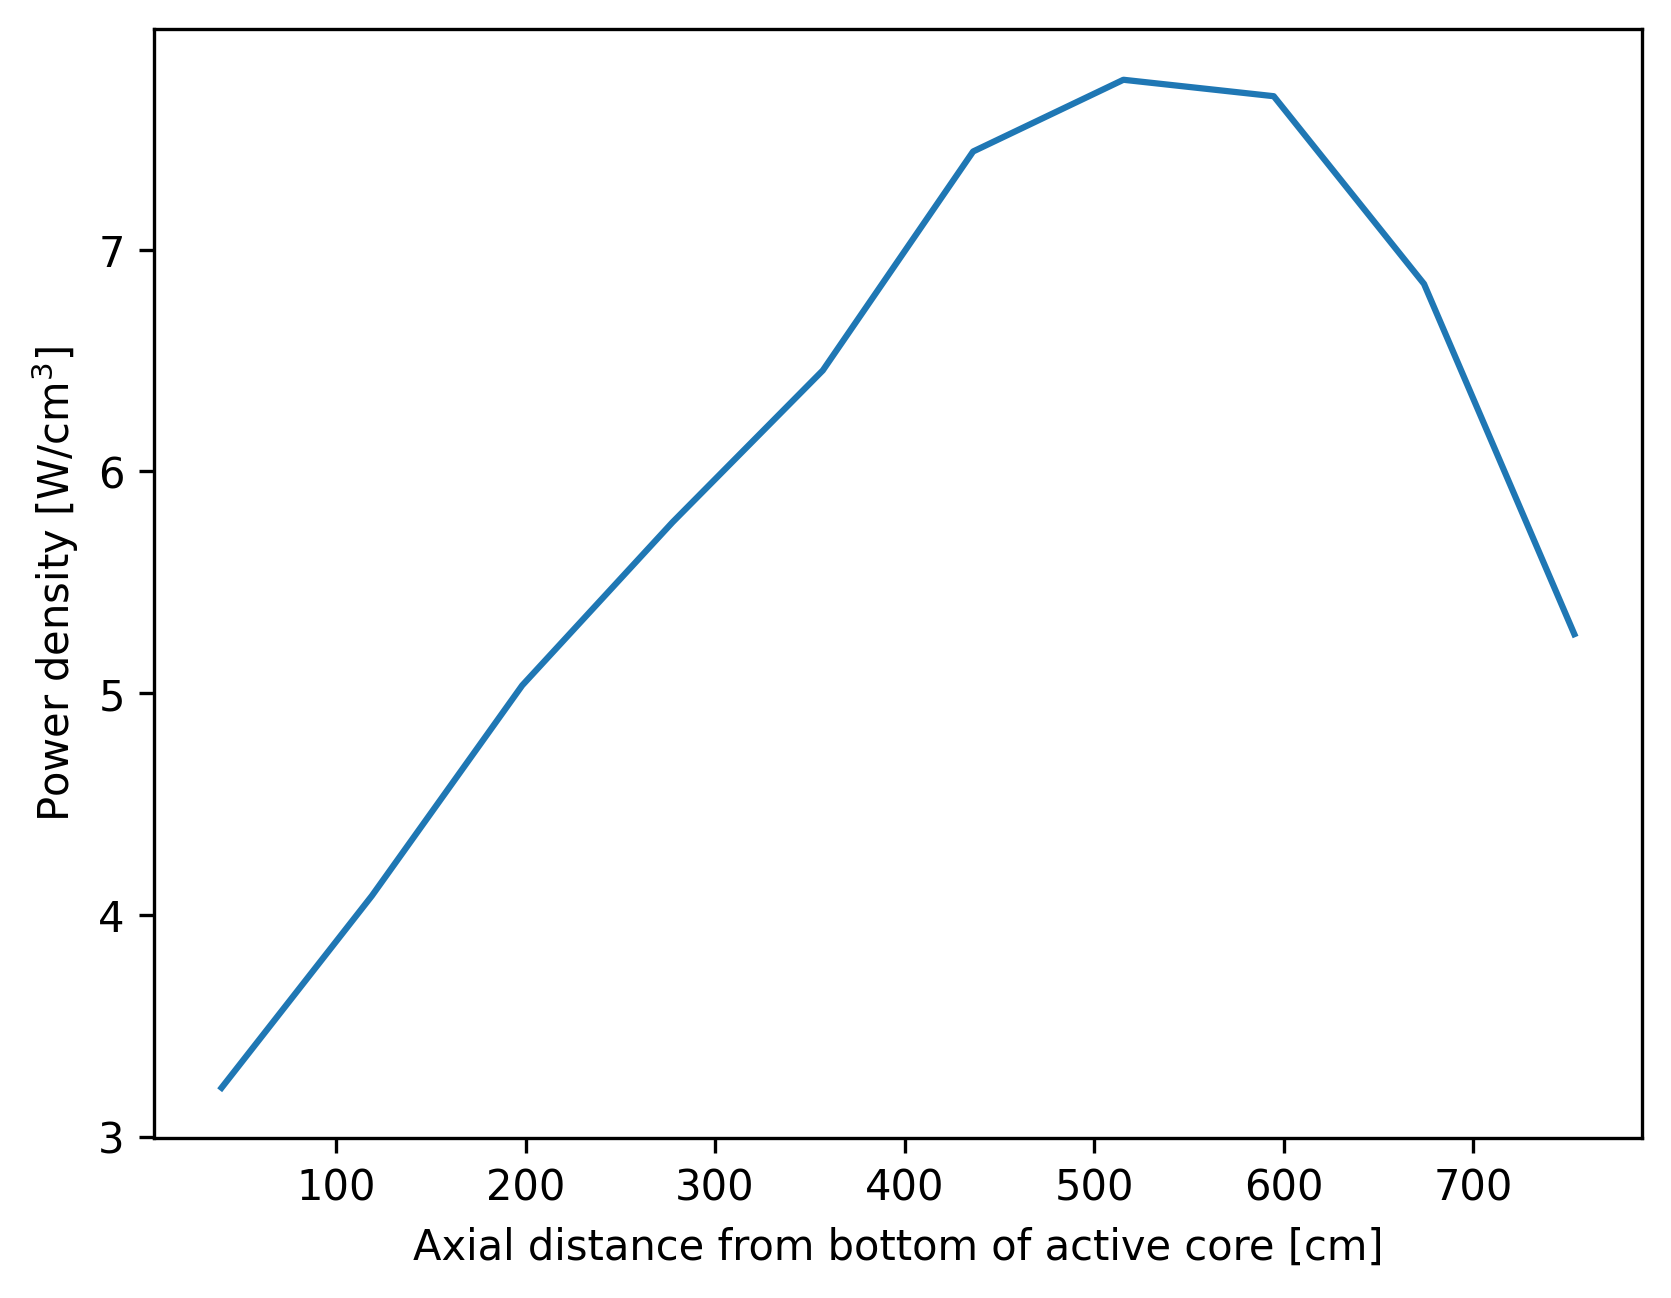
\includegraphics[width=0.42\textwidth]{figures-neutronics/3D-fullcore26G-axialpower}
    }
    \subfloat[Benchmark result. Image reproduced from \cite{oecd_nea_coupled_2020}.]{
        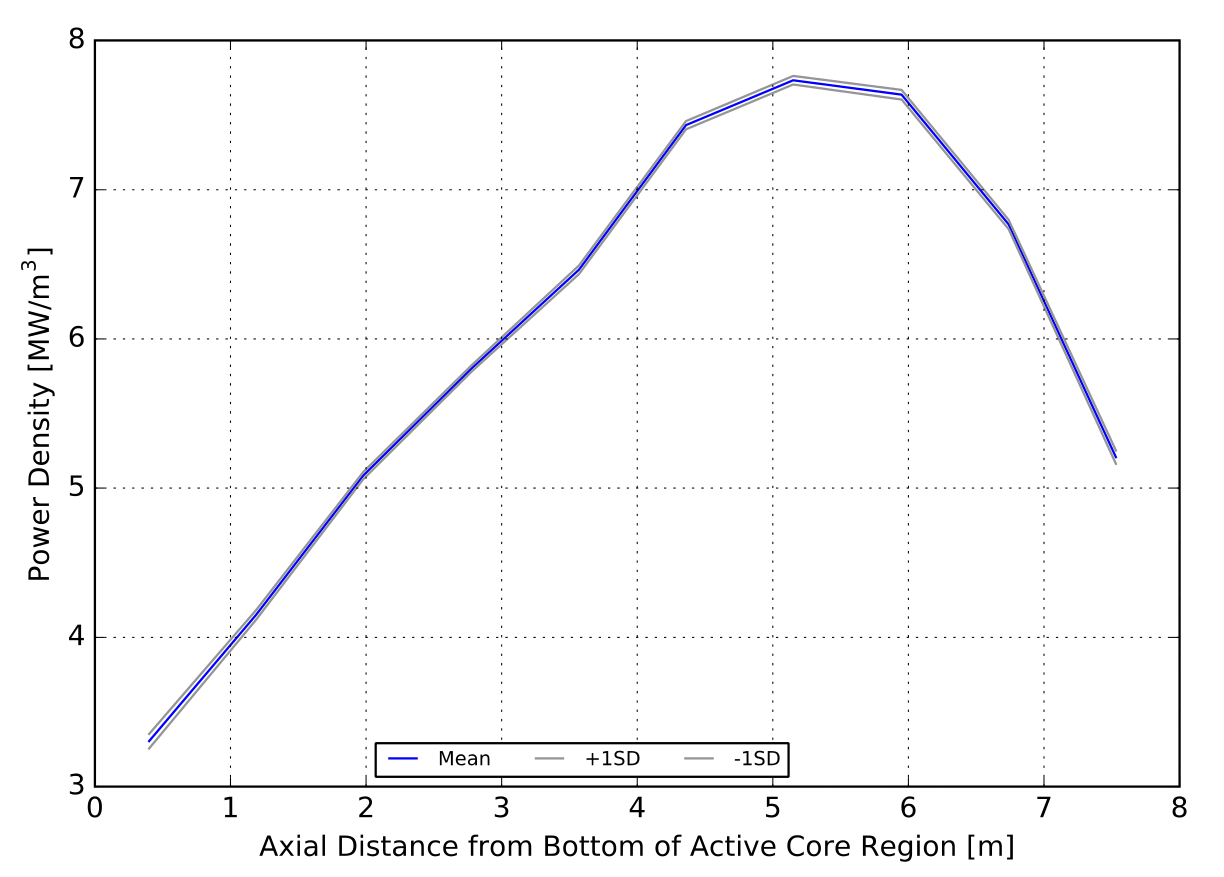
\includegraphics[width=0.47\textwidth]{figures-neutronics/benchmark-axialpower}
    }
	\hfill
	\caption{Comparison between the radially averaged axial power distribution calculated by Moltres and the benchmark published result \cite{oecd_nea_coupled_2020}.}
	\label{fig:axialpower}
\end{figure}

\begin{figure}[htbp!]
	\centering
    \subfloat[Moltres result.]{
        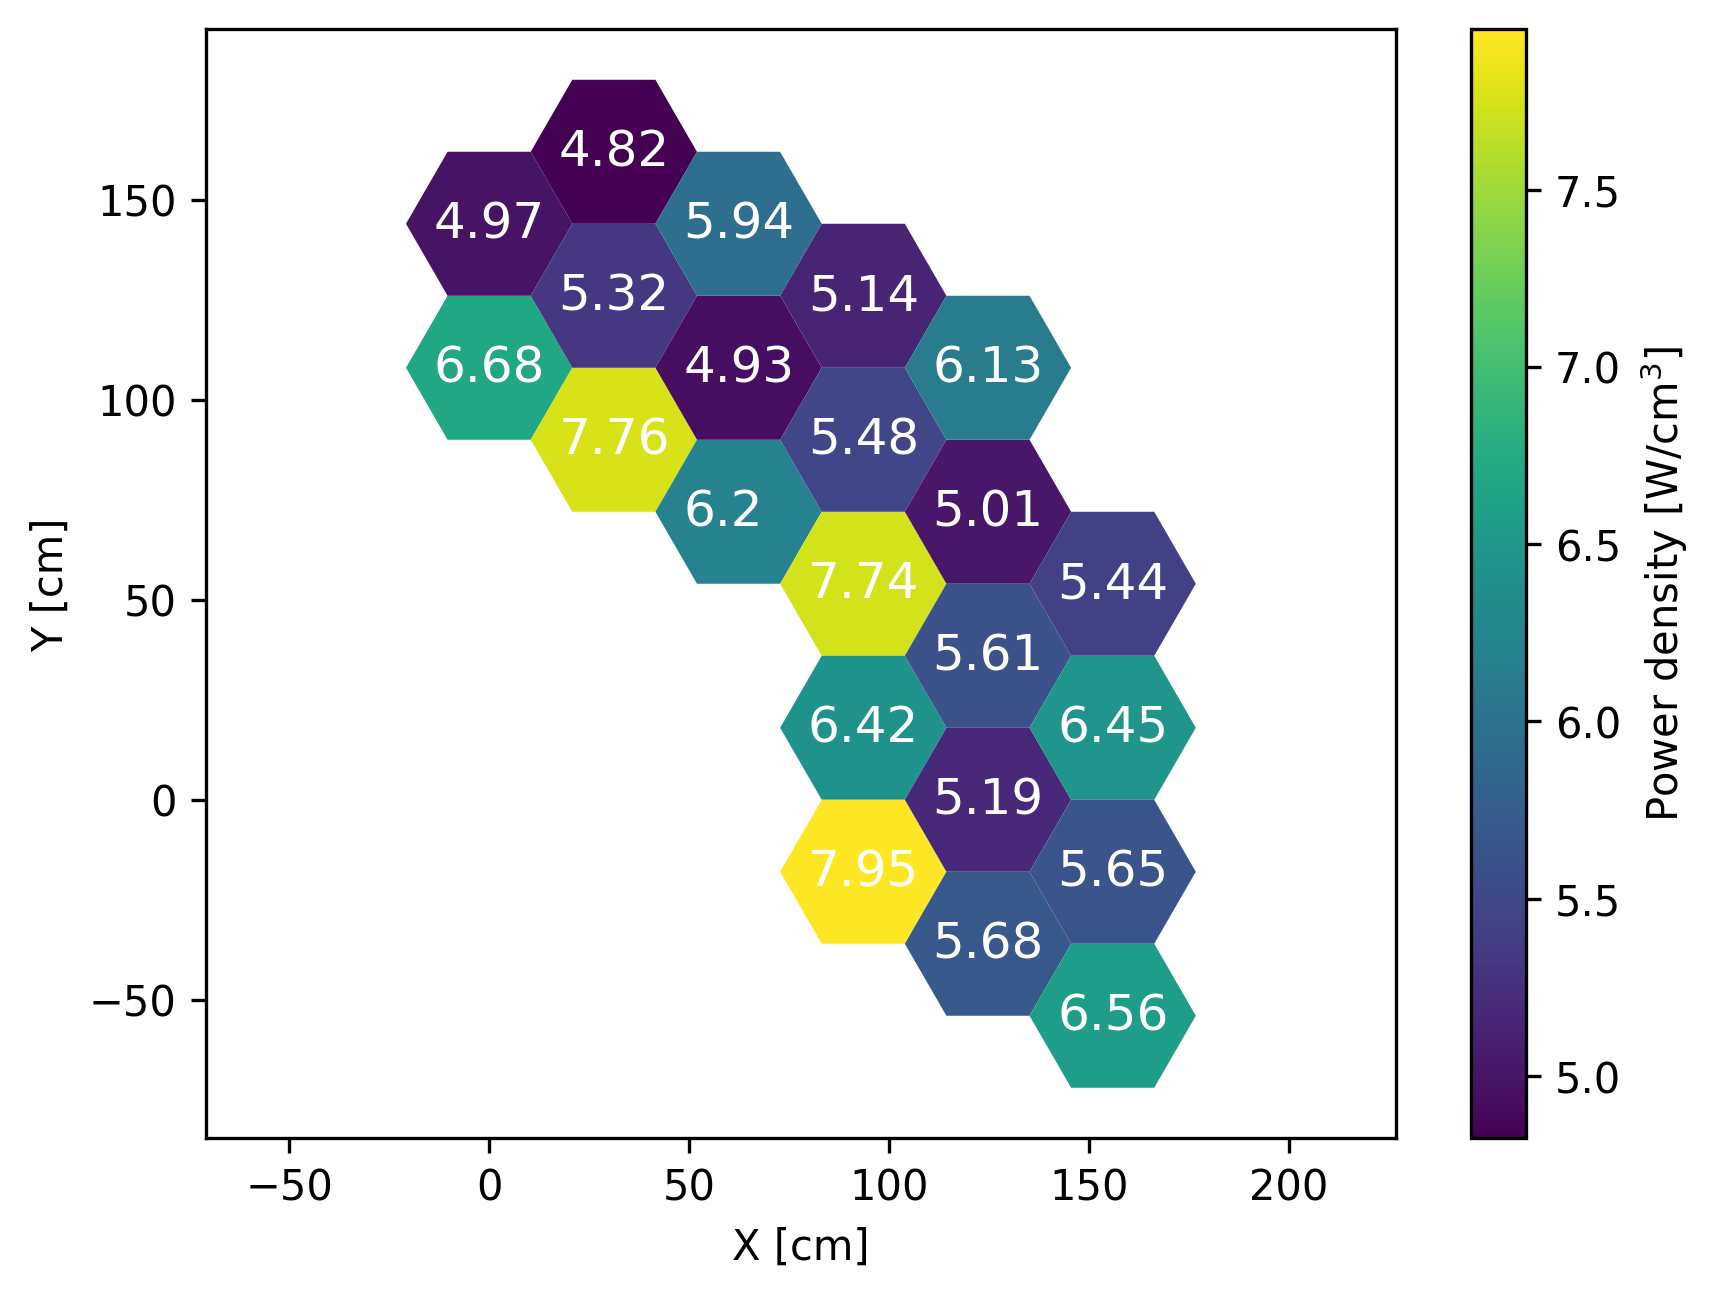
\includegraphics[width=0.47\textwidth]{figures-neutronics/3D-fullcore26G-radialpower}
    }
    \subfloat[Benchmark result. Values expressed in $MW \cdot m^{-3}$. Image reproduced from \cite{oecd_nea_coupled_2020}.]{
        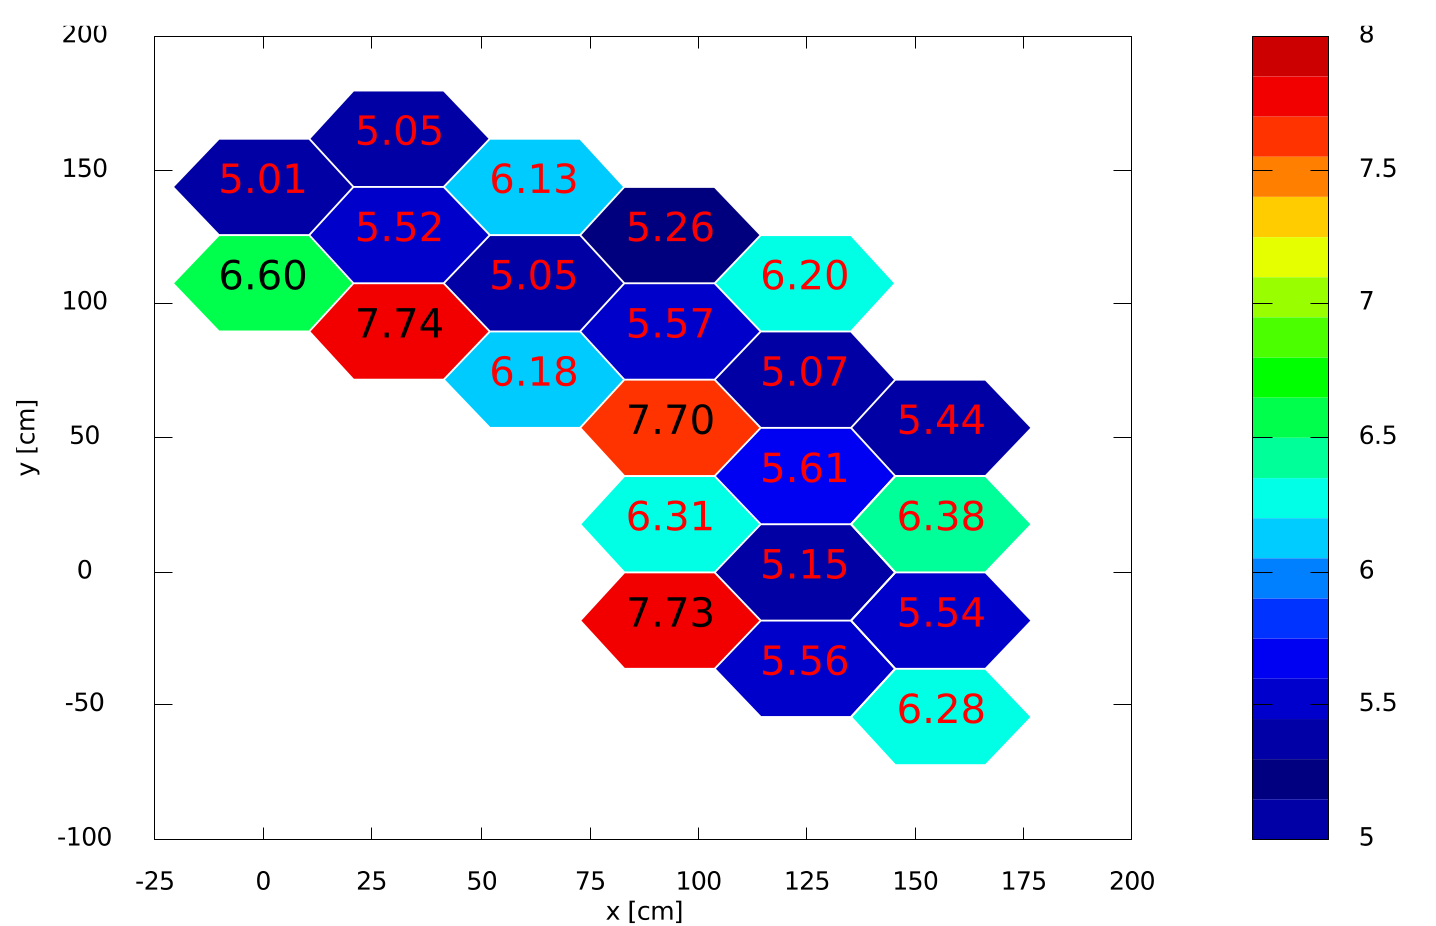
\includegraphics[width=0.42\textwidth, height=6.2cm]{figures-neutronics/benchmark-radialpower}
    }
	\hfill
  \caption{Comparison between the axially averaged radial power distribution calculated by Moltres and the benchmark published result \cite{oecd_nea_coupled_2020}.}
  \label{fig:radialpower}
\end{figure}

\subsection{Periodic vs Reflective Boundary Conditions}
\label{sec:bench-bcs}

In the last section, we observed deviations in Moltres results for the Phase I Exercise 1 of the OECD/NEA MHTGR-350 Benchmark.
This section analyzes the discrepancies that the reflective \gls{BC} approximation may have introduced in the simulations.
As the previous section mentioned, the simulation's memory requirements restrict the use of periodic BCs.
A Python script collapsed the group constants to a smaller number of energy groups to reduce the memory requirements (refer to Section \ref{appendix:group-const-condense} for further detail on group constants handling).
The simulations used 3- and 6-energy group structures (see Table \ref{tab:energygroups}).

The simulations required two meshes each: one for the control rod out and one for the control rod in.
The 3-energy group simulation had 6.2 $\times 10^4$ DoFs per energy-group (total of 1.9 $\times 10^5$ DoFs) and 6.2 $\times 10^4$ DoFs per energy-group (total of 1.8 $\times 10^5$ DoFs) for the control rod out and the control rod in simulations, respectively.
The 6-group simulation had 1.7 $\times 10^4$ DoFs per energy-group (total of 1.0 $\times 10^5$ DoFs) and 1.9 $\times 10^4$ DoFs per energy-group (total of 1.1 $\times 10^5$ DoFs) for the control out and the control rod in simulations, respectively.
The 6-group simulation had to use a coarser mesh; otherwise, it would not run.
This fact confirmed the suspicion that the simulation's memory requirements prevented it from running.

Table \ref{tab:benchmark-bc} compares the results from the simulations using periodic and reflective BCs.
k$_{eff}$ rises with the reflective BC.
With the control rod out, the raise is small, while with the control rod in, the increase is considerable.
The combined effect of both increases leads to a decrease in the control rod worth.
The BC approximation barely affects the axial offset.

\begin{table}[htbp!]
  \centering
  \caption{Global parameter comparison for different types of BCs.}
  \begin{tabular}{clcccc}
  \toprule
  Energy groups       & Type of BCs & k$_{eff, out}$ & k$_{eff, in}$ & $\Delta \rho_{CR}$ [pcm] & AO \\
  \midrule
  \multirow{2}{*}{3}  & Periodic     & 1.07571		& 1.06776		& 692.6		& 0.237		\\
                      & Reflective   & 1.07586	  & 1.07021   & 490.5		& 0.237	  \\ \hline
  \multirow{2}{*}{6}  & Periodic     & 1.07182		& 1.06356		& 724.3	  & 0.185  	\\
                      & Reflective   & 1.07197   	& 1.06610 	& 513.3		& 0.186		\\  
  \bottomrule
  \end{tabular}
  \label{tab:benchmark-bc}
\end{table}

\section{Conclusions}
\label{sec:neutr-conc}

This chapter addressed several objectives of this thesis by presenting the results of several stand-alone neutronics simulations of prismatic HTGRs using Moltres.

% Preliminary studies: homogeneous vs heterogeneous isotopic distribution
The preliminary studies focused on several aspects of the simulations.
The first aspect was the effect of distributing the fuel compact isotopes homogeneously in the Serpent model.
The results showed that the fuel compact isotopes' homogenization decreased the multiplication factor considerably and that the heterogeneous calculation took 28$\%$ longer.
These results suggest that although explicit modeling of the TRISO particles is time-consuming, it is necessary.

% Preliminary studies: homogeneous vs heterogeneous diffusion simulation
The next section studied the problem setup in Moltres.
Previous work used Moltres for simulating MSRs, which allow for heterogeneous diffusion calculations.
This work aimed to use Moltres to solve prismatic HTGRs using a heterogeneous diffusion calculation.
Nevertheless, the diffusion approximation fails to yield accurate results in regions where the mean free path is comparable to its dimensions.
The presence of helium in the prismatic HTGR fuel assembly challenges some of the diffusion theory assumptions.
Based on this discussion, this work adopted a homogeneous diffusion calculation scheme for Moltres simulations.

% Serpent-Moltres: Fuel column
Focusing on a fuel column of the MHTGR-350, Section \ref{sec:neut-fuelcol} investigated the effects of the energy group structure on the diffusion calculations.
The analysis considered four operational cases: a fuel column without burnable poisons and a fuel column with burnable poisons, both cases at 600K and 1200K.
The first study compared the axial flux calculated by Moltres to axial flux calculated by Serpent.
Overall, the axial fluxes showed good agreement.
A different study focused on the effects of the energy group structure on the \gls{Keff}.
The number of energy groups did not affect the accuracy of the Moltres eigenvalue calculations.
Another study compared the $L_2$-norm of the axial flux relative difference in the active core using various energy group structures.
For the four operational cases, increasing the number of energy groups improved accuracy.
The last study concerning the fuel column analyzed the impact of using different 15-energy group structures on the $L_2$-norm of the axial flux relative error.
The $L_2$-norm of the various operational cases responded differently to the various 15-energy group structures.
The analysis concluded that the $15d$ energy group structure was the best-performing one.

% Serpent-Moltres: Full-core
Section \ref{sec:neut-fullcore} compared Moltres full-core model results to Serpent reference results for two operational temperatures: 600K and 1200K.
The first analysis compared the eigenvalues calculated by Serpent and Moltres --- Moltres results were bigger, but the overall differences were less than 300 pcm.
The second analysis compared the radial power distributions from both applications, whose maximum relative difference was less than 7\% and located in the middle ring.
% The last analysis of the section compared Moltres and Serpent fluxes in two arbitrary core regions.
% The axial fluxes showed small discrepancies, mostly in their magnitude.
% The radial fluxes were close in shape and magnitude; however, the radial flux in the diffusion calculation failed to capture the flux variation near the burnable poisons.
% For the most part, Moltres axial and radial fluxes showed proximity to the Serpent’s results.

% OECD-Benchmark
Section \ref{sec:ph1e1} describes the results of Phase I Exercise 1 of the OECD/NEA MHTGR-350 Benchmark using Moltres.
The group constants of the exercise have a 26-energy group structure, and the exercise sets periodic \glspl{BC} on the sides of the geometry.
The simulation's high memory requirements challenged such implementation in Moltres.
The simulations approximated the periodic BC with a reflective BC to reduce the memory requirements.
Two of the global parameters ($k_{eff,out}$ and AO) exhibited good agreement with the reference results; however, the control rod worth presented a large discrepancy, resulting from the BC approximation.
Reducing the problem's size by collapsing the group constants to 3 and 6-energy groups, we compared the \gls{Keff} using the periodic and reflective BCs.
A reflective BC for the \gls{CR} out case did not substantially impact the \gls{Keff}, but the BC choice for the control rod in case had a significant effect.
A reflective BC for the \gls{CR} out case did not substantially impact the \gls{Keff}, whereas it had a significant effect of the control rod in case.
Their combined effect led to a large error in the control rod worth, while it had only a small influence on the axial offset.

This chapter met several objectives of this thesis by demonstrating Moltres' ability to predict HTGR neutronics, analyzing the impact of the energy group structure on the diffusion calculations, and illustrating Moltres' capability to calculate the power distribution of HTGRs.
